%% bare_jrnl.tex
%% V1.4b
%% 2015/08/26
%% by Michael Shell
%% see http://www.michaelshell.org/
%% for current contact information.
%%
%% This is a skeleton file demonstrating the use of IEEEtran.cls
%% (requires IEEEtran.cls version 1.8b or later) with an IEEE
%% journal paper.
%%
%% Support sites:
%% http://www.michaelshell.org/tex/ieeetran/
%% http://www.ctan.org/pkg/ieeetran
%% and
%% http://www.ieee.org/

%%*************************************************************************
%% Legal Notice:
%% This code is offered as-is without any warranty either expressed or
%% implied; without even the implied warranty of MERCHANTABILITY or
%% FITNESS FOR A PARTICULAR PURPOSE! 
%% User assumes all risk.
%% In no event shall the IEEE or any contributor to this code be liable for
%% any damages or losses, including, but not limited to, incidental,
%% consequential, or any other damages, resulting from the use or misuse
%% of any information contained here.
%%
%% All comments are the opinions of their respective authors and are not
%% necessarily endorsed by the IEEE.
%%
%% This work is distributed under the LaTeX Project Public License (LPPL)
%% ( http://www.latex-project.org/ ) version 1.3, and may be freely used,
%% distributed and modified. A copy of the LPPL, version 1.3, is included
%% in the base LaTeX documentation of all distributions of LaTeX released
%% 2003/12/01 or later.
%% Retain all contribution notices and credits.
%% ** Modified files should be clearly indicated as such, including  **
%% ** renaming them and changing author support contact information. **
%%*************************************************************************


% *** Authors should verify (and, if needed, correct) their LaTeX system  ***
% *** with the testflow diagnostic prior to trusting their LaTeX platform ***
% *** with production work. The IEEE's font choices and paper sizes can   ***
% *** trigger bugs that do not appear when using other class files.       ***                          ***
% The testflow support page is at:
% http://www.michaelshell.org/tex/testflow/



\documentclass[journal]{IEEEtran}
\usepackage{amsmath,amssymb,amsfonts}
\usepackage{algorithmic}
\usepackage{algorithm}
\usepackage{graphicx}
\usepackage{textcomp}
\usepackage{xcolor}
\usepackage{cite}
\usepackage{booktabs}
\usepackage{bm}
\usepackage{multirow}
\usepackage{url}
\usepackage{hyperref}
\usepackage{subcaption}
\newtheorem{theorem}{\bf Theorem}
\newtheorem{corollary}{\bf Corollary}
\newtheorem{remark}{\bf Remark}


%
% If IEEEtran.cls has not been installed into the LaTeX system files,
% manually specify the path to it like:
% \documentclass[journal]{../sty/IEEEtran}





% Some very useful LaTeX packages include:
% (uncomment the ones you want to load)


% *** MISC UTILITY PACKAGES ***
%
%\usepackage{ifpdf}
% Heiko Oberdiek's ifpdf.sty is very useful if you need conditional
% compilation based on whether the output is pdf or dvi.
% usage:
% \ifpdf
%   % pdf code
% \else
%   % dvi code
% \fi
% The latest version of ifpdf.sty can be obtained from:
% http://www.ctan.org/pkg/ifpdf
% Also, note that IEEEtran.cls V1.7 and later provides a builtin
% \ifCLASSINFOpdf conditional that works the same way.
% When switching from latex to pdflatex and vice-versa, the compiler may
% have to be run twice to clear warning/error messages.






% *** CITATION PACKAGES ***
%
%\usepackage{cite}
% cite.sty was written by Donald Arseneau
% V1.6 and later of IEEEtran pre-defines the format of the cite.sty package
% \cite{} output to follow that of the IEEE. Loading the cite package will
% result in citation numbers being automatically sorted and properly
% "compressed/ranged". e.g., [1], [9], [2], [7], [5], [6] without using
% cite.sty will become [1], [2], [5]--[7], [9] using cite.sty. cite.sty's
% \cite will automatically add leading space, if needed. Use cite.sty's
% noadjust option (cite.sty V3.8 and later) if you want to turn this off
% such as if a citation ever needs to be enclosed in parenthesis.
% cite.sty is already installed on most LaTeX systems. Be sure and use
% version 5.0 (2009-03-20) and later if using hyperref.sty.
% The latest version can be obtained at:
% http://www.ctan.org/pkg/cite
% The documentation is contained in the cite.sty file itself.






% *** GRAPHICS RELATED PACKAGES ***
%
\ifCLASSINFOpdf
  % \usepackage[pdftex]{graphicx}
  % declare the path(s) where your graphic files are
  % \graphicspath{{../pdf/}{../jpeg/}}
  % and their extensions so you won't have to specify these with
  % every instance of \includegraphics
  % \DeclareGraphicsExtensions{.pdf,.jpeg,.png}
\else
  % or other class option (dvipsone, dvipdf, if not using dvips). graphicx
  % will default to the driver specified in the system graphics.cfg if no
  % driver is specified.
  % \usepackage[dvips]{graphicx}
  % declare the path(s) where your graphic files are
  % \graphicspath{{../eps/}}
  % and their extensions so you won't have to specify these with
  % every instance of \includegraphics
  % \DeclareGraphicsExtensions{.eps}
\fi
% graphicx was written by David Carlisle and Sebastian Rahtz. It is
% required if you want graphics, photos, etc. graphicx.sty is already
% installed on most LaTeX systems. The latest version and documentation
% can be obtained at: 
% http://www.ctan.org/pkg/graphicx
% Another good source of documentation is "Using Imported Graphics in
% LaTeX2e" by Keith Reckdahl which can be found at:
% http://www.ctan.org/pkg/epslatex
%
% latex, and pdflatex in dvi mode, support graphics in encapsulated
% postscript (.eps) format. pdflatex in pdf mode supports graphics
% in .pdf, .jpeg, .png and .mps (metapost) formats. Users should ensure
% that all non-photo figures use a vector format (.eps, .pdf, .mps) and
% not a bitmapped formats (.jpeg, .png). The IEEE frowns on bitmapped formats
% which can result in "jaggedy"/blurry rendering of lines and letters as
% well as large increases in file sizes.
%
% You can find documentation about the pdfTeX application at:
% http://www.tug.org/applications/pdftex





% *** MATH PACKAGES ***
%
%\usepackage{amsmath}
% A popular package from the American Mathematical Society that provides
% many useful and powerful commands for dealing with mathematics.
%
% Note that the amsmath package sets \interdisplaylinepenalty to 10000
% thus preventing page breaks from occurring within multiline equations. Use:
%\interdisplaylinepenalty=2500
% after loading amsmath to restore such page breaks as IEEEtran.cls normally
% does. amsmath.sty is already installed on most LaTeX systems. The latest
% version and documentation can be obtained at:
% http://www.ctan.org/pkg/amsmath





% *** SPECIALIZED LIST PACKAGES ***
%
%\usepackage{algorithmic}
% algorithmic.sty was written by Peter Williams and Rogerio Brito.
% This package provides an algorithmic environment fo describing algorithms.
% You can use the algorithmic environment in-text or within a figure
% environment to provide for a floating algorithm. Do NOT use the algorithm
% floating environment provided by algorithm.sty (by the same authors) or
% algorithm2e.sty (by Christophe Fiorio) as the IEEE does not use dedicated
% algorithm float types and packages that provide these will not provide
% correct IEEE style captions. The latest version and documentation of
% algorithmic.sty can be obtained at:
% http://www.ctan.org/pkg/algorithms
% Also of interest may be the (relatively newer and more customizable)
% algorithmicx.sty package by Szasz Janos:
% http://www.ctan.org/pkg/algorithmicx




% *** ALIGNMENT PACKAGES ***
%
%\usepackage{array}
% Frank Mittelbach's and David Carlisle's array.sty patches and improves
% the standard LaTeX2e array and tabular environments to provide better
% appearance and additional user controls. As the default LaTeX2e table
% generation code is lacking to the point of almost being broken with
% respect to the quality of the end results, all users are strongly
% advised to use an enhanced (at the very least that provided by array.sty)
% set of table tools. array.sty is already installed on most systems. The
% latest version and documentation can be obtained at:
% http://www.ctan.org/pkg/array


% IEEEtran contains the IEEEeqnarray family of commands that can be used to
% generate multiline equations as well as matrices, tables, etc., of high
% quality.




% *** SUBFIGURE PACKAGES ***
%\ifCLASSOPTIONcompsoc
%  \usepackage[caption=false,font=normalsize,labelfont=sf,textfont=sf]{subfig}
%\else
%  \usepackage[caption=false,font=footnotesize]{subfig}
%\fi
% subfig.sty, written by Steven Douglas Cochran, is the modern replacement
% for subfigure.sty, the latter of which is no longer maintained and is
% incompatible with some LaTeX packages including fixltx2e. However,
% subfig.sty requires and automatically loads Axel Sommerfeldt's caption.sty
% which will override IEEEtran.cls' handling of captions and this will result
% in non-IEEE style figure/table captions. To prevent this problem, be sure
% and invoke subfig.sty's "caption=false" package option (available since
% subfig.sty version 1.3, 2005/06/28) as this is will preserve IEEEtran.cls
% handling of captions.
% Note that the Computer Society format requires a larger sans serif font
% than the serif footnote size font used in traditional IEEE formatting
% and thus the need to invoke different subfig.sty package options depending
% on whether compsoc mode has been enabled.
%
% The latest version and documentation of subfig.sty can be obtained at:
% http://www.ctan.org/pkg/subfig




% *** FLOAT PACKAGES ***
%
%\usepackage{fixltx2e}
% fixltx2e, the successor to the earlier fix2col.sty, was written by
% Frank Mittelbach and David Carlisle. This package corrects a few problems
% in the LaTeX2e kernel, the most notable of which is that in current
% LaTeX2e releases, the ordering of single and double column floats is not
% guaranteed to be preserved. Thus, an unpatched LaTeX2e can allow a
% single column figure to be placed prior to an earlier double column
% figure.
% Be aware that LaTeX2e kernels dated 2015 and later have fixltx2e.sty's
% corrections already built into the system in which case a warning will
% be issued if an attempt is made to load fixltx2e.sty as it is no longer
% needed.
% The latest version and documentation can be found at:
% http://www.ctan.org/pkg/fixltx2e


%\usepackage{stfloats}
% stfloats.sty was written by Sigitas Tolusis. This package gives LaTeX2e
% the ability to do double column floats at the bottom of the page as well
% as the top. (e.g., "\begin{figure*}[!b]" is not normally possible in
% LaTeX2e). It also provides a command:
%\fnbelowfloat
% to enable the placement of footnotes below bottom floats (the standard
% LaTeX2e kernel puts them above bottom floats). This is an invasive package
% which rewrites many portions of the LaTeX2e float routines. It may not work
% with other packages that modify the LaTeX2e float routines. The latest
% version and documentation can be obtained at:
% http://www.ctan.org/pkg/stfloats
% Do not use the stfloats baselinefloat ability as the IEEE does not allow
% \baselineskip to stretch. Authors submitting work to the IEEE should note
% that the IEEE rarely uses double column equations and that authors should try
% to avoid such use. Do not be tempted to use the cuted.sty or midfloat.sty
% packages (also by Sigitas Tolusis) as the IEEE does not format its papers in
% such ways.
% Do not attempt to use stfloats with fixltx2e as they are incompatible.
% Instead, use Morten Hogholm'a dblfloatfix which combines the features
% of both fixltx2e and stfloats:
%
% \usepackage{dblfloatfix}
% The latest version can be found at:
% http://www.ctan.org/pkg/dblfloatfix




%\ifCLASSOPTIONcaptionsoff
%  \usepackage[nomarkers]{endfloat}
% \let\MYoriglatexcaption\caption
% \renewcommand{\caption}[2][\relax]{\MYoriglatexcaption[#2]{#2}}
%\fi
% endfloat.sty was written by James Darrell McCauley, Jeff Goldberg and 
% Axel Sommerfeldt. This package may be useful when used in conjunction with 
% IEEEtran.cls'  captionsoff option. Some IEEE journals/societies require that
% submissions have lists of figures/tables at the end of the paper and that
% figures/tables without any captions are placed on a page by themselves at
% the end of the document. If needed, the draftcls IEEEtran class option or
% \CLASSINPUTbaselinestretch interface can be used to increase the line
% spacing as well. Be sure and use the nomarkers option of endfloat to
% prevent endfloat from "marking" where the figures would have been placed
% in the text. The two hack lines of code above are a slight modification of
% that suggested by in the endfloat docs (section 8.4.1) to ensure that
% the full captions always appear in the list of figures/tables - even if
% the user used the short optional argument of \caption[]{}.
% IEEE papers do not typically make use of \caption[]'s optional argument,
% so this should not be an issue. A similar trick can be used to disable
% captions of packages such as subfig.sty that lack options to turn off
% the subcaptions:
% For subfig.sty:
% \let\MYorigsubfloat\subfloat
% \renewcommand{\subfloat}[2][\relax]{\MYorigsubfloat[]{#2}}
% However, the above trick will not work if both optional arguments of
% the \subfloat command are used. Furthermore, there needs to be a
% description of each subfigure *somewhere* and endfloat does not add
% subfigure captions to its list of figures. Thus, the best approach is to
% avoid the use of subfigure captions (many IEEE journals avoid them anyway)
% and instead reference/explain all the subfigures within the main caption.
% The latest version of endfloat.sty and its documentation can obtained at:
% http://www.ctan.org/pkg/endfloat
%
% The IEEEtran \ifCLASSOPTIONcaptionsoff conditional can also be used
% later in the document, say, to conditionally put the References on a 
% page by themselves.




% *** PDF, URL AND HYPERLINK PACKAGES ***
%
%\usepackage{url}
% url.sty was written by Donald Arseneau. It provides better support for
% handling and breaking URLs. url.sty is already installed on most LaTeX
% systems. The latest version and documentation can be obtained at:
% http://www.ctan.org/pkg/url
% Basically, \url{my_url_here}.




% *** Do not adjust lengths that control margins, column widths, etc. ***
% *** Do not use packages that alter fonts (such as pslatex).         ***
% There should be no need to do such things with IEEEtran.cls V1.6 and later.
% (Unless specifically asked to do so by the journal or conference you plan
% to submit to, of course. )


% correct bad hyphenation here
\hyphenation{op-tical net-works semi-conduc-tor}


\begin{document}
%
% paper title
% Titles are generally capitalized except for words such as a, an, and, as,
% at, but, by, for, in, nor, of, on, or, the, to and up, which are usually
% not capitalized unless they are the first or last word of the title.
% Linebreaks \\ can be used within to get better formatting as desired.
% Do not put math or special symbols in the title.
\title{DARS: Task Demand-Attentive Reinforcement Scheduling for Wireless-Powered Multi-UAV Mobile Edge Computing}
%
%
% author names and IEEE memberships
% note positions of commas and nonbreaking spaces ( ~ ) LaTeX will not break
% a structure at a ~ so this keeps an author's name from being broken across
% two lines.
% use \thanks{} to gain access to the first footnote area
% a separate \thanks must be used for each paragraph as LaTeX2e's \thanks
% was not built to handle multiple paragraphs
%

\author{Chenlu Li, 
        Xiaoyu Wang,~\IEEEmembership{Member,~IEEE,}
        He Huang,~\IEEEmembership{Senior Member,~IEEE,}
        and Haipeng Dai,~\IEEEmembership{Senior Member,~IEEE}% <-this % stops a space
\IEEEcompsocitemizethanks{\IEEEcompsocthanksitem
This research was funded by the National Natural Science Foundation of China (Grant No. 62202321 and 62332013).
\IEEEcompsocthanksitem C. Li, X. Wang, and H. Huang are with the School of Computer Science and Technology, Soochow University, Suzhou 215006, Jiangsu, P. R. China. E-mails: cllichenluli@stu.suda.edu.cn, \{xywang21, huangh\}@suda.edu.cn
\IEEEcompsocthanksitem H. Dai is with State Key Laboratory for Novel Software Technology, Nanjing University, Nanjing 210023, Jiangsu, P. R. China. E-mail: haipengdai@nju.edu.cn.
}% <-this % stops a space
\thanks{Corresponding Author: X. Wang (xywang21@suda.edu.cn).}}

% note the % following the last \IEEEmembership and also \thanks - 
% these prevent an unwanted space from occurring between the last author name
% and the end of the author line. i.e., if you had this:
% 
% \author{....lastname \thanks{...} \thanks{...} }
%                     ^------------^------------^----Do not want these spaces!
%
% a space would be appended to the last name and could cause every name on that
% line to be shifted left slightly. This is one of those "LaTeX things". For
% instance, "\textbf{A} \textbf{B}" will typeset as "A B" not "AB". To get
% "AB" then you have to do: "\textbf{A}\textbf{B}"
% \thanks is no different in this regard, so shield the last } of each \thanks
% that ends a line with a % and do not let a space in before the next \thanks.
% Spaces after \IEEEmembership other than the last one are OK (and needed) as
% you are supposed to have spaces between the names. For what it is worth,
% this is a minor point as most people would not even notice if the said evil
% space somehow managed to creep in.



% The paper headers
\markboth{IEEE Internet of Things Journal,~Vol.~xx, No.~xx, August~2026}%
{Li \MakeLowercase{\textit{et al.}}: DARS: Task Demand-Attentive Reinforcement Scheduling for Wireless-Powered Multi-UAV Mobile Edge Computing}
% The only time the second header will appear is for the odd numbered pages
% after the title page when using the twoside option.
% 
% *** Note that you probably will NOT want to include the author's ***
% *** name in the headers of peer review papers.                   ***
% You can use \ifCLASSOPTIONpeerreview for conditional compilation here if
% you desire.




% If you want to put a publisher's ID mark on the page you can do it like
% this:
%\IEEEpubid{0000--0000/00\$00.00~\copyright~2015 IEEE}
% Remember, if you use this you must call \IEEEpubidadjcol in the second
% column for its text to clear the IEEEpubid mark.



% use for special paper notices
%\IEEEspecialpapernotice{(Invited Paper)}




% make the title area
\maketitle

% As a general rule, do not put math, special symbols or citations
% in the abstract or keywords.
\begin{abstract}
Unmanned aerial vehicles (UAVs) equipped with mobile edge computing (MEC) servers can act as aerial edge nodes to provide on-demand computation offloading for ground Internet of Things devices, especially where terrestrial infrastructure is unavailable or costly. However, limited onboard energy, stochastic task arrivals, and time-varying demand hinder sustainable service provision. This paper investigates task-demand-aware scheduling in a wireless-powered multi-UAV MEC system in which UAVs serve ground users and replenish energy through wireless charging towers. We formulate a joint scheduling problem that coordinates UAV movement, task offloading, user association, computation allocation, and bandwidth allocation to maximize service latency reduction subject to long-term energy feasibility. We develop a \underline{D}emand-\underline{A}ttentive \underline{R}einforcement \underline{S}cheduling (DARS) framework based on deep reinforcement learning. The outer layer combines soft actor-critic with a task-demand attention encoder to learn long-term movement and offloading policies; the middle layer uses marginal-SLRR greedy user association with bounded move/swap improvement; and the inner layer uses convex optimization to derive square-root closed-form computation and bandwidth allocations. DARS further integrates dual-priority prioritized experience replay and $n$-step returns to emphasize transitions with large temporal-difference errors or reward variation caused by demand shifts and energy-critical states. Simulation results show that DARS outperforms representative deep
reinforcement learning benchmarks in terms of cumulative reward, service
latency reduction ratio, and average task completion latency under varying
user densities and hotspot intensities.
\end{abstract}
% Note that keywords are not normally used for peerreview papers.
\begin{IEEEkeywords}
Mobile Edge Computing, Wireless Charging, Deep Reinforcement Learning, Prioritized Experience Replay, Convex Optimization.
\end{IEEEkeywords}






% For peer review papers, you can put extra information on the cover
% page as needed:
% \ifCLASSOPTIONpeerreview
% \begin{center} \bfseries EDICS Category: 3-BBND \end{center}
% \fi
%
% For peerreview papers, this IEEEtran command inserts a page break and
% creates the second title. It will be ignored for other modes.
\IEEEpeerreviewmaketitle



\section{Introduction}
% The very first letter is a 2 line initial drop letter followed
% by the rest of the first word in caps.
% 
% form to use if the first word consists of a single letter:
% \IEEEPARstart{A}{demo} file is ....
% 
% form to use if you need the single drop letter followed by
% normal text (unknown if ever used by the IEEE):
% \IEEEPARstart{A}{}demo file is ....
% 
% Some journals put the first two words in caps:
% \IEEEPARstart{T}{his demo} file is ....
% 
% Here we have the typical use of a "T" for an initial drop letter
% and "HIS" in caps to complete the first word.
\IEEEPARstart{W}{ith} the proliferation of Internet of Things (IoT) devices and the emergence of computation-intensive applications such as augmented reality, real-time video analytics, and autonomous driving~\cite{wang2023wpmec_survey, 
ning2025joint_data}, the demand for ubiquitous and low-latency computing services has increased rapidly. Mobile Edge Computing (MEC) has emerged as a highly promising paradigm, effectively alleviating the computational burden on resource-constrained user equipment (UE) by providing cloud-like computing capabilities at the network edge. However, in scenarios such as disaster relief, remote areas, or temporary hotspots, deploying fixed MEC infrastructure is often economically prohibitive or physically infeasible. Consequently, Unmanned Aerial Vehicles (UAVs) are increasingly integrated into MEC networks~\cite{zeng2019energy,wu2018joint, hao2024joint_tmc}. Benefiting from their agile mobility, flexible deployment capabilities, and favorable Line-of-Sight (LoS) communication links, UAVs equipped with lightweight servers can serve as aerial edge nodes. By dynamically adjusting their trajectories to approach active users, they can significantly reduce communication latency and enhance the overall Quality of Service (QoS).


However, the limited onboard energy of UAVs remains a critical bottleneck for long-term service provisioning. Unlike terrestrial edge servers powered by stable energy supplies, UAVs must consume their limited battery energy for flying, hovering, and computation. Once the battery is depleted, the UAV has to terminate its mission, leading to service interruption and degraded QoS. Wireless Power Transfer (WPT) has recently been considered as an effective solution to prolong UAV operation~\cite{xu2018uav, 
ning2025joint_data}, where Wireless Charging Towers (WCTs) deployed on rooftops or elevated platforms can replenish UAV energy during hovering~\cite{xu2018uav}. Nevertheless, the introduction of WCTs also changes the nature of UAV scheduling: UAVs are no longer required to only approach users for better offloading performance, but also need to periodically move toward WCTs for energy replenishment.

Therefore, this paper investigates the problem of task demand-aware reinforcement scheduling for wireless-powered multi-UAV MEC, aiming to jointly optimize UAV movement, task offloading, user association, and resource allocation to reduce user service latency while sustaining long-term UAV operation.


There are three main challenges in this problem. First, the introduction of WCTs creates a service-charging tradeoff~\cite{song2024energy}. UAVs need to fly close to active users to improve computation offloading efficiency, while also approaching WCTs before energy depletion to maintain continuous service. Second, user task demands are spatially uneven and time-varying. Due to stochastic task arrivals and hotspot migration~\cite{wang2021dynamic_imitation}, UAVs must dynamically adjust their trajectories and offloading decisions according to the changing demand distribution. Third, the system involves heterogeneous and tightly coupled decisions~\cite{wang2024joint}. UAV trajectory planning and task offloading are long-term continuous-control decisions, user association is a discrete matching decision, and computation and bandwidth allocation need to be efficiently determined within each time slot. These coupled factors make the original optimization problem difficult to solve directly.

Motivated by the success of Deep Reinforcement Learning (DRL) in solving high-dimensional and dynamic decision-making problems, we develop a DRL-based scheduling framework for wireless-powered multi-UAV MEC. Specifically, we propose a Demand-Attentive Reinforcement Scheduling framework, called DARS, which combines Soft Actor-Critic (SAC), Prioritized Experience Replay (PER), task-demand attention, and closed-form resource allocation. The SAC-based controller is adopted to improve exploration in continuous UAV movement and offloading action spaces~\cite{haarnoja2018soft}, while PER is introduced to enhance the learning of rare but informative transitions such as energy-critical states and sudden demand changes~\cite{schaul2016per}. Furthermore, a task-demand attention mechanism is designed to extract demand-aware user representations, and closed-form resource allocation is derived to reduce the computational burden within each time slot.

The main contributions of this paper are summarized as follows.
\begin{itemize}
\item  We develop DARS, a cascaded scheduling architecture that separates long-term UAV movement and task-offloading decisions, feasible user association, and instantaneous resource allocation. Its middle layer ranks feasible user--UAV associations by their marginal change in the current sum-SLRR objective, then applies bounded move/swap improvement while respecting coverage and capacity constraints.
\item We design a task-demand attention encoder to construct a permutation-invariant global representation of the user-demand configuration. We further develop a dual-priority replay rule that combines temporal-difference error and reward variation with $n$-step returns, thereby emphasizing demand shifts and energy-critical transitions.
\item We establish the strict convexity of the computation and bandwidth allocation subproblems and derive square-root closed-form solutions through the Karush-Kuhn-Tucker conditions. These solutions avoid including instantaneous resource variables in the reinforcement-learning action space.
\item We evaluate the proposed framework through extensive simulations against
mainstream stochastic, deterministic and multi-agent policy baselines. DARS
attains higher cumulative reward, a larger service latency reduction ratio and
a lower average task completion latency, and the advantage is retained as the
user density and the hotspot intensity vary. Ablation results further indicate
that the demand-attentive representation and the dual-priority replay rule
contribute to the performance gain and to the post-convergence stability,
respectively.

\end{itemize}


\section{Related Work}

\subsection{UAV-Assisted Mobile Edge Computing}

UAV-assisted Mobile Edge Computing has attracted 
increasing attention due to its flexible deployment and strong 
capability to provide on-demand computing services. Existing 
studies have investigated UAV trajectory design, communication 
scheduling, computation offloading, and resource allocation 
from different perspectives. For example, trajectory and 
communication co-design has been studied to improve the 
performance of UAV-enabled wireless networks~\cite{zeng2019energy, 
wu2018joint}. In UAV-assisted MEC systems, deep reinforcement 
learning and stochastic optimization methods have also been 
adopted to jointly optimize task offloading and UAV movement 
under dynamic environments~\cite{jie2020drl, zhang2018stochastic}. 
In addition, the communication and computation aspects of MEC 
have been extensively surveyed in~\cite{mao2017survey}, providing 
important foundations for computation offloading and edge 
resource allocation. 
More recently, multi-agent DRL has been applied to multi-UAV 
MEC systems with cooperative offloading and trajectory 
control~\cite{lee2024marl, li2024robust, wang2024joint}. 
Specifically, \cite{lee2024marl} jointly controls offloading 
ratios and UAV trajectories via multi-agent reinforcement 
learning, but does not consider energy replenishment. 
The work in~\cite{li2024robust} studies robust computation 
offloading and trajectory optimization under uncertain channel 
conditions, yet assumes stationary user distributions. 
In~\cite{wang2024joint}, joint user association, trajectory, 
offloading, and resource allocation are investigated in 
air-ground cooperative MEC, but the long-term energy 
sustainability of UAVs is not addressed.

However, most existing UAV-MEC studies mainly focus on 
improving short-term offloading efficiency or reducing task 
completion latency under a given energy budget. The long-term 
sustainability of UAV services is often treated as an energy 
constraint rather than a key scheduling objective. In contrast, 
this paper considers a wireless-powered multi-UAV MEC scenario, 
where UAVs must learn how to balance task service and energy 
replenishment to maintain continuous operation.

\subsection{Wireless-Powered UAV Networks}

Wireless Power Transfer has been introduced into UAV 
networks as a promising technique to extend UAV operation time. 
Existing works have studied UAV-enabled wireless power transfer, 
trajectory design, and energy optimization in different wireless 
charging scenarios~\cite{xu2018uav, griffin2012resonant, 
hu2019optimal}. In addition, practical wireless charger 
deployment and heterogeneous charging models have been 
investigated to improve the feasibility of wireless charging 
systems~\cite{wang2020practical}. 
More recent studies have explored the integration of wireless 
charging into UAV-MEC scheduling. 
In~\cite{zeng2023joint}, joint resource allocation and 
trajectory optimization are studied for wirelessly-powered 
UAV-MEC in large-area scenarios, but the scheduling relies on 
convex relaxation without learning-based adaptation. 
The work in~\cite{song2024energy} applies multi-objective 
reinforcement learning to energy-efficient trajectory 
optimization with wireless charging, though the approach does 
not incorporate demand-aware state representations. 
In~\cite{pan2023joint}, joint power and 3D trajectory 
optimization is investigated for UAV-enabled wireless powered 
communication networks with obstacles. 
Furthermore, \cite{fu2024computation} studies computation 
energy-efficiency fairness in UAV-enabled wireless-powered MEC 
networks with hybrid passive and active transmissions.
DRL has also been applied to online computation offloading in wireless-powered
MEC networks~\cite{huang2020drl_wpmec}, although without UAV mobility.


Nevertheless, most WPT-related UAV studies focus on 
communication or energy transfer performance, while computation 
offloading and edge resource scheduling are less explored. 
Moreover, many works rely on pre-planned trajectories or 
relatively static service environments, which may not adapt 
well to stochastic task arrivals and time-varying user hotspots. 
Different from these studies, this paper integrates WPT-enabled 
energy replenishment into a multi-UAV MEC system and studies 
the joint scheduling of UAV movement, task offloading, user 
association, and resource allocation under dynamic task demand.
\subsection{DRL-Based UAV Scheduling}

Deep Reinforcement Learning has shown strong potential 
in solving high-dimensional sequential decision-making problems 
in wireless networks~\cite{luong2019applications}. In UAV 
systems, DRL has been applied to trajectory control, 
communication scheduling, and computation 
offloading~\cite{jie2020drl, zhang2018stochastic}, while 
multi-agent actor-critic methods provide useful tools for 
cooperative decision-making~\cite{lowe2017multi}. Compared with 
conventional optimization methods, DRL can learn adaptive 
policies through interaction with dynamic environments, making 
it suitable for UAV-MEC systems with stochastic task arrivals 
and user mobility. Meanwhile, advanced DRL techniques such as 
maximum-entropy learning and prioritized experience replay have 
been proposed to improve exploration and sample 
efficiency~\cite{haarnoja2018soft, schaul2016per}. 
Recent advances have further explored more sophisticated 
architectures for DRL-based UAV scheduling. 
A comprehensive survey on reinforcement learning for autonomous 
multi-UAV wireless networks is presented 
in~\cite{bai2023towards}, covering trajectory design, resource 
management, and cooperative control. 
The work in~\cite{he2024deep} studies distributed 3D UAV 
trajectory design with deep reinforcement learning under 
non-stationary environments. 
In addition, \cite{consul2024hybrid} introduces a digital-twin 
empowered UAV-MEC framework with federated reinforcement 
learning for adaptive task offloading and resource allocation.
Attention mechanisms have also been introduced into edge-computing scheduling
to encode inter-device correlations~\cite{li2023task,wang2024tfddrl} and into
multi-UAV multi-server task offloading~\cite{chen2024attention_offloading}.
These works mainly attend over servers or candidate actions, whereas the
proposed TDA encoder attends over ground users to produce a
permutation-invariant, demand-aware representation whose weights follow the
spatio-temporal migration of task hotspots.


However, directly applying standard DRL algorithms to 
wireless-powered multi-UAV MEC still faces several limitations. 
First, energy depletion is a rare but critical event, and its 
impact on long-term service performance may not be effectively 
learned through uniform experience replay. Second, dynamic task 
hotspots can cause sudden changes in system rewards, but such 
transitions may be insufficiently emphasized by conventional 
replay mechanisms. Third, flat state representations may dilute 
the information of active users when the number of ground users 
is large. To address these issues, DARS combines demand-aware 
state representation, dual-priority experience replay, and 
cascaded decision decomposition, enabling UAVs to learn 
sustainable service-charging behaviors while improving latency 
reduction performance.

% \begin{table}[!t]
% \renewcommand{\arraystretch}{1.15}
% \caption{Summary of Main Notations}
% \label{tab:notation}
% \centering
% \footnotesize
% \begin{tabular}{p{0.20\columnwidth}p{0.70\columnwidth}}
% \hline
% \textbf{Notation} & \textbf{Description}\\
% \hline
% $\mathcal{K}=\{u_1,\dots,u_K\}$ & Set of $K$ UAVs; $u_k$ denotes the $k$-th UAV\\
% $\mathcal{M}=\{m_1,\dots,m_M\}$ & Set of $M$ ground users; $m_i$ denotes the $i$-th GU\\
% $\mathcal{W}=\{w_1,\dots,w_{N_w}\}$ & Set of $N_w$ WCTs; $w_j$ denotes the $j$-th WCT\\
% $\mathfrak{C}=\{\mathcal{C}_1,\dots,\mathcal{C}_{N_c}\}$ & Collection of $N_c$ user clusters\\
% $\mathcal{T}\triangleq\{1,\dots,T\}$ & Index set of time slots (a pure index set)\\
% $\mathcal{U}_k(t),\mathcal{U}^{+}_k(t)$ & Users served by $u_k$ / active offloading users of $u_k$\\
% $\mathcal{H}(t)\subseteq\mathfrak{C}$ & Set of hotspot clusters in slot $t$\\
% $L,\;H,\;H_c$ & Side length of the square service area; UAV altitude; WCT altitude\\
% $\bm{q}_k(t)$ & Horizontal position of $u_k$\\
% $\bm{p}_i(t)$ & Horizontal position of $m_i$\\
% $\bm{\mu}_{g(i)}$ & Reference centre of the cluster containing $m_i$\\
% $\bm{c}_j$ & Horizontal position of $w_j$\\
% $\sigma_c$ & Spatial dispersion (std.) of the RPGM model\\
% $\lambda_i(t),\xi_i(t)$ & Task arrival probability / task activation indicator of $m_i$\\
% $D_i(t),\;\phi,\;C_i(t)$ & Task data size; computation intensity; workload $C_i(t)=D_i(t)\phi$\\
% $x_i(t)$ & Offloading ratio of $m_i$, $x_i(t)\in[0,1]$\\
% $a_{i,k}(t)$ & Association indicator between $m_i$ and $u_k$\\
% $f_{i,k}(t),b_{i,k}(t)$ & CPU frequency / bandwidth allocated by $u_k$ to $m_i$\\
% $F_{\mathrm{UAV}},W_{\mathrm{tot}}$ & Total CPU capacity and bandwidth of one UAV\\
% $f_{\mathrm{UE}},P_{tx}$ & Local CPU frequency; user transmit power\\
% $v_k(t),\varphi_k(t)$ & Flight speed and heading angle of $u_k$\\
% $d_{i,k}(t),\vartheta_{i,k}(t)$ & UAV--GU 3-D distance and elevation angle\\
% $\ell_{j,k}(t),L_c$ & UAV--WCT 3-D distance; charging coverage radius\\
% $B_k(t),B_{\max}$ & Residual / maximum battery energy\\
% $\rho_i(t)$ & Service latency reduction ratio (SLRR) of $m_i$\\
% $s_t,a_t,r_t$ & MDP state, action and reward at slot $t$\\
% $\bm{h}_t$ & Demand-aware representation produced by the TDA encoder\\
% $\delta_z,\varpi_z,p_z$ & TD error, IS weight and priority of the $z$-th transition\\
% \hline
% \end{tabular}
% \end{table}

\section{System Model and Problem Formulation}\label{sec:model}
\subsection{System Model}
As shown in Fig.~\ref{fig:system}, we consider a multi-UAV-assisted mobile edge computing
system integrated with WPT over a square service area of size $L\times L$~m$^2$.
The system comprises three categories of entities: a set of $K$ UAVs equipped
with MEC servers, denoted by $\mathcal{K}=\{u_1,u_2,\ldots,u_K\}$, where $u_k$
represents the $k$-th UAV, all flying at a fixed altitude $H$ to provide
computation offloading services for ground users; a set of $M$ ground users
(GUs), denoted by $\mathcal{M}=\{m_1,m_2,\ldots,m_M\}$, where $m_i$ represents
the $i$-th GU generating computation-intensive tasks that can be partially
offloaded to the UAVs; and a set of $N_w$ wireless charging towers (WCTs),
denoted by $\mathcal{W}=\{\mathsf{w}_1,\mathsf{w}_2,\ldots,\mathsf{w}_{N_w}\}$, where
$\mathsf{w}_j$ represents the $j$-th WCT. Throughout this paper, calligraphic
letters denote sets of entities, while $\{1,\ldots,K\}$, $\{1,\ldots,M\}$ and
$\{1,\ldots,N_w\}$ are used only as subscript index ranges.

% Throughout this paper, calligraphic letters denote
% sets of entities, and the index sets $\{1,\ldots,K\}$, $\{1,\ldots,M\}$,
% $\{1,\ldots,N_w\}$ are used only as subscript ranges. The total service horizon
% is divided into $T$ equal time slots indexed by
% $\mathcal{T}\triangleq\{1,2,\ldots,T\}$.

\begin{figure}[t]
\centering
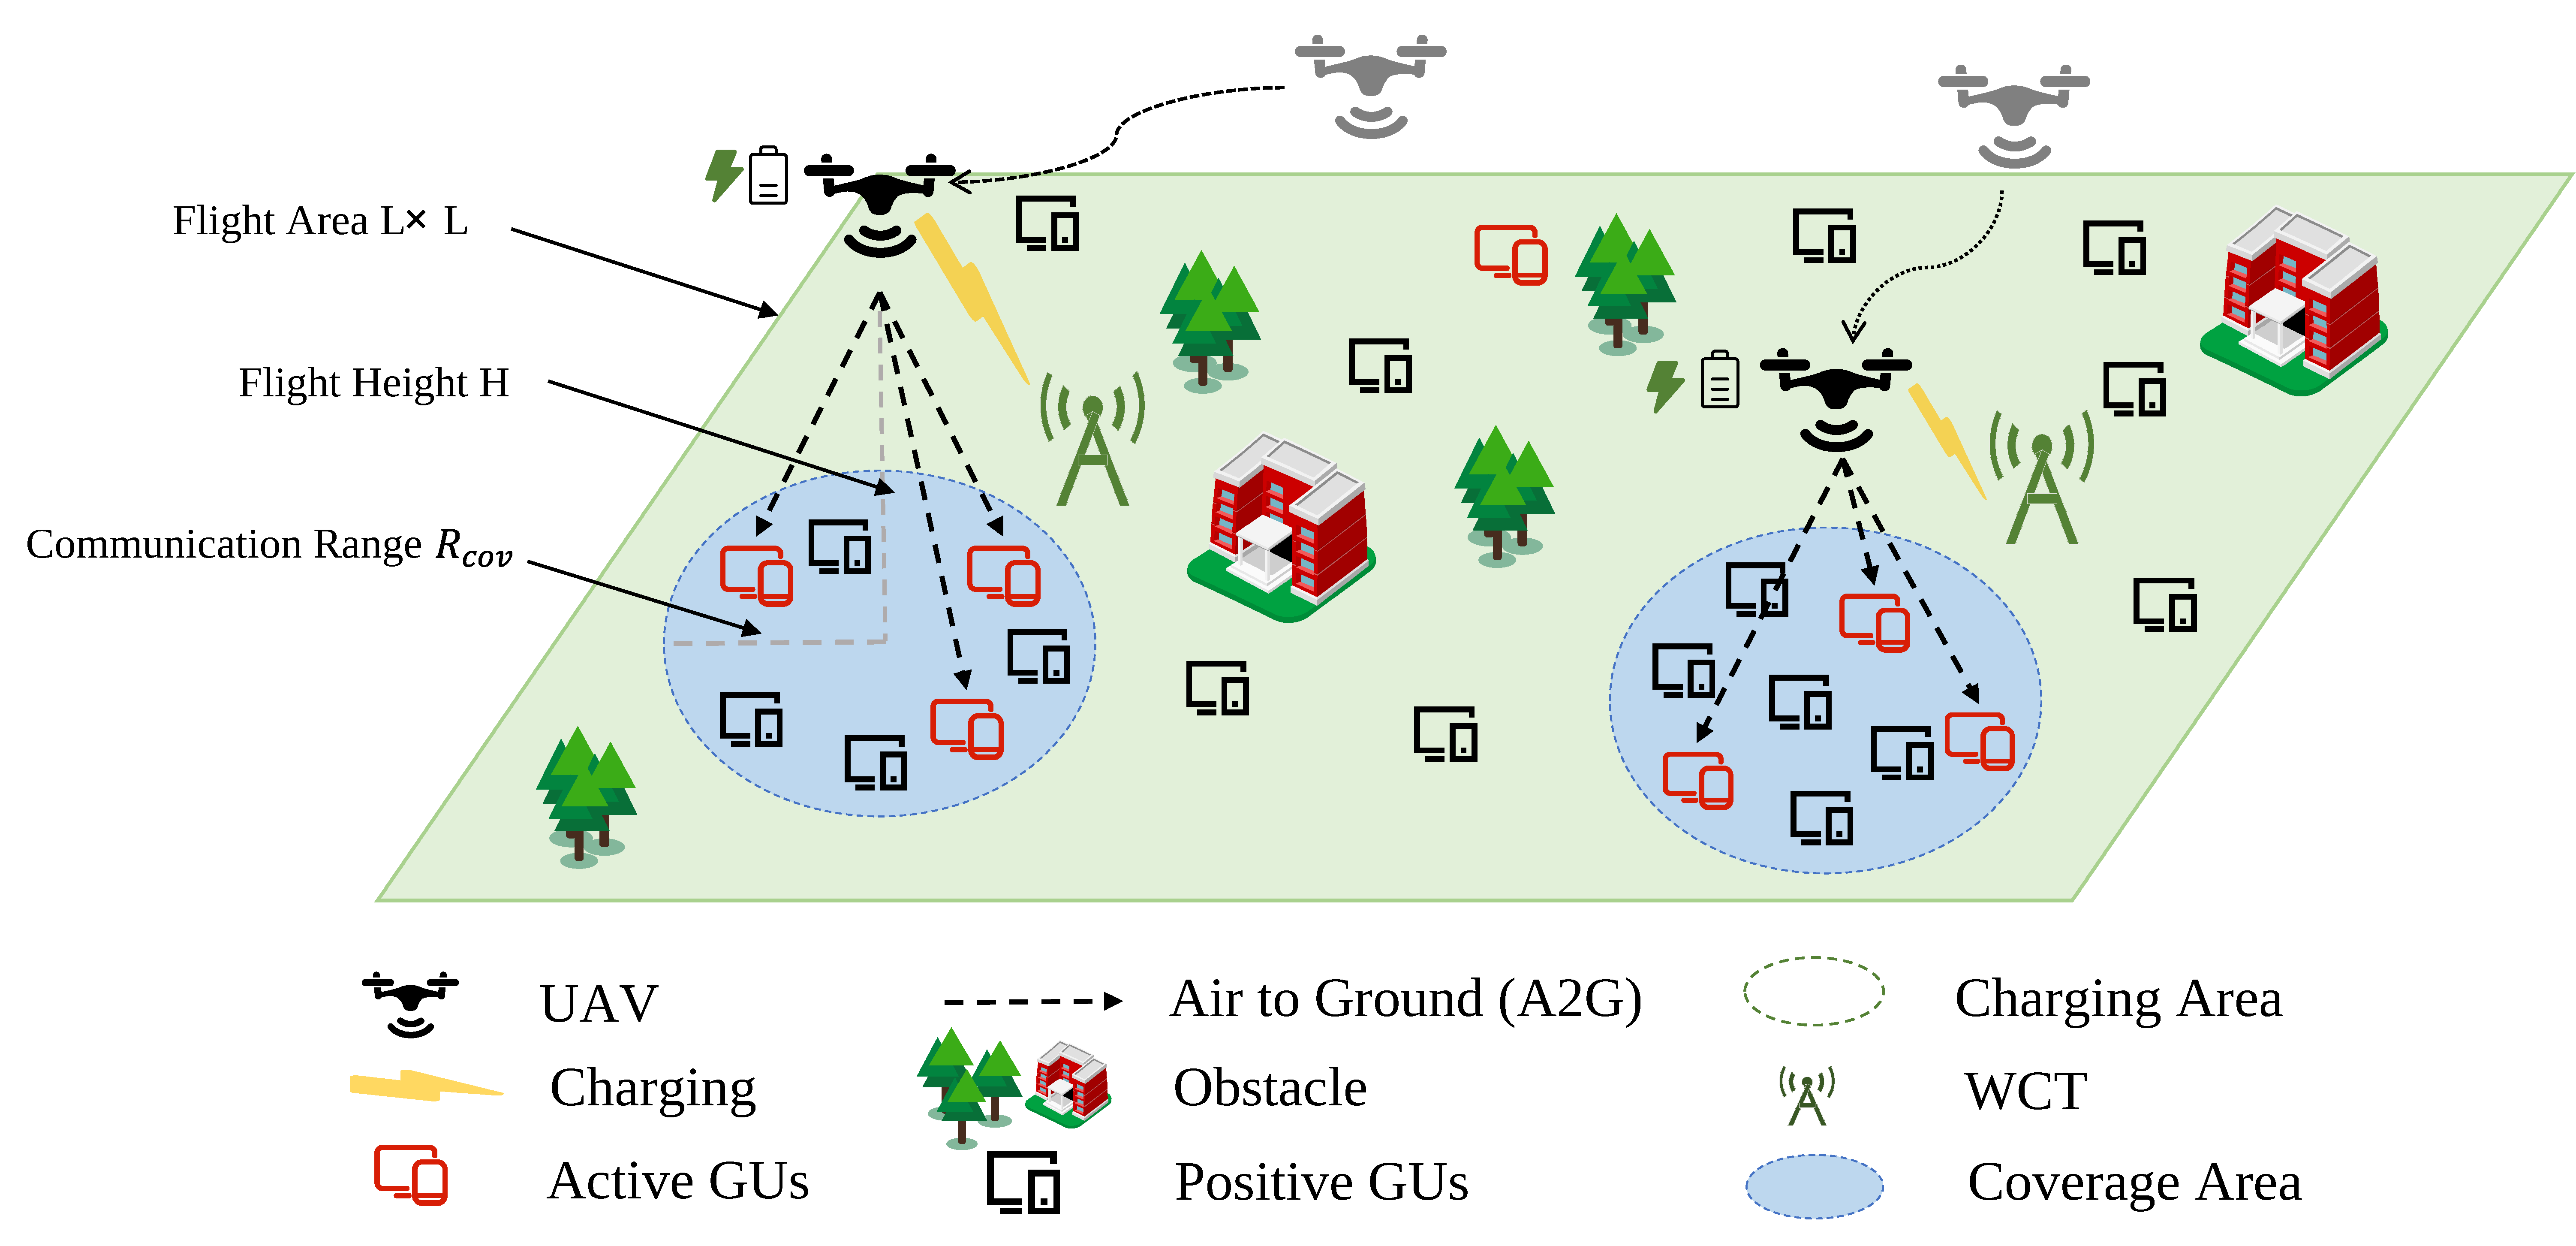
\includegraphics[width=\linewidth]{fig/picture2_vector.pdf}
\caption{Architecture of the wireless-powered multi-UAV MEC system.}
\label{fig:system}
\end{figure}

% Let
% \(\mathcal{I}_k^{+}(t)=\{i_1,i_2,\ldots,i_n\}\), where
% \(n=|\mathcal{I}_k^{+}(t)|\), and define
% \[
% \bm{f}
% =
% [f_{i_1,k},f_{i_2,k},\ldots,f_{i_n,k}]^{\mathsf T}.
% \]

The total service horizon is divided into \(T\) equal time slots.
Following the fly-then-hover protocol~\cite{zeng2019energy}, each time slot
consists of two phases: a flight phase with duration \(T_{\mathrm{fly}}\),
followed by a service phase with duration \(T_{\mathrm{com}}\). At the
beginning of slot \(t\), UAV \(u_k\) is located at \(\bm q_k(t)\). Given its
flight speed \(v_k(t)\) and heading angle \(\varphi_k(t)\), the tentative
position after the flight phase is
\begin{equation}\label{eq:uav_tentative_motion}
\tilde{\bm q}_k(t+1)
=
\bm q_k(t)
+
v_k(t)T_{\mathrm{fly}}
\begin{bmatrix}
\cos\varphi_k(t)\\
\sin\varphi_k(t)
\end{bmatrix}.
\end{equation}
To keep the UAV inside the square service area, a mirror-reflection boundary
rule is applied whenever the tentative trajectory crosses the boundary.
Accordingly, the updated position is
\begin{equation}\label{eq:uav_motion}
\bm q_k(t+1)
=
\mathcal{R}_{[0,L]^2}
\bigl(\tilde{\bm q}_k(t+1)\bigr),
\end{equation}
where \(\mathcal{R}_{[0,L]^2}(\cdot)\) reflects an out-of-bound coordinate
symmetrically with respect to the corresponding boundary. During the
subsequent service phase, the UAV hovers at \(\bm q_k(t+1)\) to perform user
association, task offloading, edge computation, and wireless energy
harvesting from nearby WCTs. The duration of each time slot is
\(\tau=T_{\mathrm{fly}}+T_{\mathrm{com}}\).



\subsubsection{Task Distribution Model}
To characterize the spatio-temporal heterogeneity of user computation demands, the system partitions the $M$ ground users into $N_c$ spatial clusters, denoted
by $\{\mathcal{C}_0,\mathcal{C}_1,\ldots,\mathcal{C}_{N_c-1}\}$. The cluster
index of $m_i$ is denoted by $g(i)$, i.e., $m_i\in\mathcal{C}_{g(i)}$. In time
slot $t$, the location of $m_i$ is generated around the reference point
$\bm{\mu}_{g(i)}$ according to the Reference Point Group Mobility (RPGM)
model~\cite{hong1999group_rpgm}:
\begin{equation}\label{eq:rpgm}
\bm{p}_i(t) = \bm{\mu}_{g(i)} + \bm{n}_i(t),\qquad
\bm{n}_i(t)\sim\mathcal{N}(\bm{0},\sigma_c^{2}\bm{I}_2),
\end{equation}
where $\bm{\mu}_{g(i)}\in\mathbb{R}^{2}$ is the reference point of the cluster
containing $m_i$, $\bm{n}_i(t)$ is a two-dimensional zero-mean Gaussian
displacement, $\sigma_c^{2}$ is the mobility variance, and $\bm{I}_2$ is the
$2\times 2$ identity matrix.


Based on the spatial clustering, the system introduces a multi-stage hot-cold cluster rotation mechanism to simulate time-varying computation hotspots. Let $\mathcal{H}(t)\subseteq\{\mathcal{C}_0,\ldots,\mathcal{C}_{N_c-1}\}$ denote the set of hotspot  clusters in time slot $t$. In each stage, a subset of clusters is selected as hotspots, while the remaining
clusters are regarded as cold spots. The set of hotspot clusters rotates clockwise across different stages. The task arrival probability of user $i$ is given by:
% \begin{equation}\label{eq:arrival}
% \lambda_i(t) = \begin{cases}
% p_{\mathrm{hot}}, & g(i) \in \mathcal{H}(t), \\
% p_{\mathrm{cold}}, & g(i) \notin \mathcal{H}(t),
% \end{cases}
% \end{equation}
% $p_{\mathrm{cold}}, \quad g(i)\in\mathcal{H}/(t)$
% →
% $p_{\mathrm{cold}}, \quad \mathcal{C}_{g(i)}\notin\mathcal{H}(t)$
\begin{equation}
\lambda_i(t)=
\begin{cases}
p_{\mathrm{hot}}, & \mathcal{C}_{g(i)}\in\mathcal{H}(t),\\[2pt]
p_{\mathrm{cold}}, & \mathcal{C}_{g(i)}\notin\mathcal{H}(t),
\end{cases}
\end{equation}
where $p_{\mathrm{hot}} > p_{\mathrm{cold}}$. The task activation indicator variable is generated via a Bernoulli distribution: $\xi_i(t) \sim \mathrm{Bernoulli}(\lambda_i(t))$. Let $a_{i,k}(t)\in\{0,1\}$ indicate whether $m_i$ is associated with $u_k$ in
time slot $t$. The set of users served by $u_k$ is defined as
$\mathcal{S}_k(t)=\{m_i\in\mathcal{M}: a_{i,k}(t)=1\}$.


\subsubsection{UAV Energy Consumption Model}

Based on the rotary-wing aerodynamics model derived in~\cite{zeng2019energy}, the propulsion power of a UAV flying at speed $v$ is given by
\begin{align}\label{eq:flypower}
P_{\mathrm{fly}}(v) &= P_0\left(1 + \frac{3v^2}{U_{\mathrm{tip}}^2}\right)
+ P_{\mathrm{ind}}\left(\sqrt{1 + \frac{v^4}{4v_0^4}} - \frac{v^2}{2v_0^2}\right)^{\frac{1}{2}} \notag \\
&\quad + \frac{1}{2} d_0 \rho_{\mathrm{air}} s_0 A_{\mathrm{rot}} v^3,
\end{align}
% where $P_0$ and $P_i$ correspond to the blade profile power and induced power in hovering status, respectively; $v_0$ is the mean rotor induced velocity in hover; $U_{\mathrm{tip}}$ denotes the tip speed of the rotor blade; $s_0$ and $\rho$ represent the rotor solidity and air density, respectively; $d_0$ and $A$ are the fuselage drag ratio and rotor disc area, respectively. The propulsion energy consumed during the flight phase of 
% slot~$t$ is thus $E_k^{\mathrm{fly}}(t) = P_{\mathrm{fly}}(v_k(t))\, 
% T_{\mathrm{fly}}$.
% Hovering corresponds to $v=0$, so the hovering power is
% $P_{\mathrm{hov}}=P_{\mathrm{fly}}(0)=P_0+P_i$ and the hovering energy consumed
% during the service phase is $E_k^{\mathrm{hov}}(t)=P_{\mathrm{hov}}T_{\mathrm{com}}$.
where $P_{\mathrm{fly}}(v)$ is the propulsion power at flight speed $v$;
$P_0$ and $P_{\mathrm{ind}}$ are the blade profile power and the induced power
in hovering status, respectively; $v_0$ is the mean rotor induced velocity in
hover; $U_{\mathrm{tip}}$ is the tip speed of the rotor blade; $s_0$ and
$\rho_{\mathrm{air}}$ are the rotor solidity and the air density; and $d_0$ and
$A_{\mathrm{rot}}$ are the fuselage drag ratio and the rotor disc area.
Let $v_k(t)\in[0,V_{\max}]$ denote the flight speed of $u_k$ in slot $t$; the
propulsion energy consumed during the flight phase is
$E^{\mathrm{fly}}_k(t)=P_{\mathrm{fly}}(v_k(t))T_{\mathrm{fly}}$. Hovering
corresponds to $v=0$, so the hovering power is
$P_{\mathrm{hov}}=P_{\mathrm{fly}}(0)=P_0+P_{\mathrm{ind}}$ and the hovering
energy consumed during the service phase is
$E^{\mathrm{hov}}_k(t)=P_{\mathrm{hov}}T_{\mathrm{com}}$.



The computation energy consumed by UAV $k$ follows the dynamic voltage and frequency scaling (DVFS) model~\cite{burd2000processor_dvfs}:
\begin{equation}\label{eq:compenergy}
E_{k}^{\mathrm{comp}}(t) \equiv \sum_{i\in \mathcal{S}_{k}^{+}(t)} \kappa f_{i,k}^{2}(t) x_{i}(t) C_{i}(t)
\end{equation}
where $\kappa$ is the effective switched capacitance coefficient determined by
the chip architecture, $D_i(t)$ is the input data size of the task
generated by $m_i$, $x_i(t)\in[0,1]$ is its offloading ratio, $f_{i,k}(t)$ is
the CPU frequency allocated by $u_k$ to $m_i$, and $C_i(t)=D_i(t)\phi$ is the
computation workload with $\phi$ the computation intensity in cycles per bit.



% The communication energy consumed by UAV~$k$ for receiving 
% uplink offloaded data during the service phase is
% \begin{equation}
%   E_k^{\mathrm{comm}}(t) = P_{\mathrm{rx}} 
%   \sum_{i \in \mathcal{S}_k(t)} 
%   \frac{\xi_i(t)\, x_i(t)\, D_i(t)}{R_{i,k}(t)},
% \end{equation}
% where $P_{\mathrm{rx}}$ is the reception circuit power of the 
% onboard receiver.



\subsubsection{Channel Model}

% The probabilistic line-of-sight (LoS) channel model proposed in~\cite{alhourani2014optimal,azari2018uav_los} is adopted.
% % The elevation angle between UAV $k$ and user $i$ is $\varphi_{i,k}(t) = \frac{180}{\pi} \arcsin\!\left(\frac{H}{d_{i,k}(t)}\right)$, and the probability of establishing an LoS link is given by
% The elevation angle between UAV $k$ and user $i$ is $\varphi_{i,k}(t) = \frac{180}{\pi} \arcsin\!\left(\frac{H}{d_{i,k}(t)}\right)$, and the probability of establishing an LoS link is given by
% \begin{equation}\label{eq:losprob}
% P_{i,k}^{\mathrm{LoS}}(t) = \frac{1}{1 + a_e \exp(-b_e(\varphi_{i,k}(t) - a_e))}.
% \end{equation}

The probabilistic line-of-sight (LoS) channel model proposed
in~\cite{alhourani2014optimal,azari2018uav_los} is adopted. The
three-dimensional distance between $u_k$ and $m_i$ is
\begin{equation}\label{eq:dist_uav_gu}
d_{i,k}(t)=\sqrt{\left\|\bm{q}_k(t)-\bm{p}_i(t)\right\|_2^{2}+H^{2}},
\end{equation}
and the corresponding elevation angle is
$\vartheta_{i,k}(t)=\frac{180}{\pi}\arcsin\!\left(H/d_{i,k}(t)\right)$ in
degrees. The probability of establishing an LoS link is given by
\begin{equation}\label{eq:losprob}
P_{i,k}^{\mathrm{LoS}}(t) = \frac{1}{1 + a_e \exp(-b_e(\vartheta_{i,k}(t) - a_e))}.
\end{equation}

The expected channel gain is expressed as
% \begin{equation}\label{eq:channel}
% g_{i,k}(t) = K_0^{-1} d_{i,k}^{-\alpha}(t) \bigl(P_{i,k}^{\mathrm{LoS}}(t) \mu_{\mathrm{LoS}} + P_{i,k}^{\mathrm{NLoS}}(t) \mu_{\mathrm{NLoS}}\bigr)^{-1},
% \end{equation}
% where $K_0 = (4\pi f_c / c)^2$ and $\alpha$ denotes the path loss exponent, $a_e,b_e$ are environment-dependent constants, $P^{\mathrm{NLoS}}_{i,k}(t)=1-P^{\mathrm{LoS}}_{i,k}(t)$.
%>> [FIX-8] alpha -> alpha_pl（避与 alpha_H/alpha_per/alpha_a/alpha_c 冲突）；补 f_c、c、mu_LoS、mu_NLoS 定义
\begin{equation}\label{eq:channel}
g_{i,k}(t) = K_0^{-1} d_{i,k}^{-\alpha_{\mathrm{pl}}}(t) \bigl(P_{i,k}^{\mathrm{LoS}}(t) \mu_{\mathrm{LoS}} + P_{i,k}^{\mathrm{NLoS}}(t) \mu_{\mathrm{NLoS}}\bigr)^{-1},
\end{equation}
where $K_0=(4\pi f_c/c)^{2}$ is the reference path loss at unit distance, with
$f_c$ the carrier frequency and $c$ the speed of light; $\alpha_{\mathrm{pl}}$
is the path loss exponent; $a_e$ and $b_e$ are environment-dependent constants
determined by the building density and height distribution;
$P^{\mathrm{NLoS}}_{i,k}(t)=1-P^{\mathrm{LoS}}_{i,k}(t)$; and
$\mu_{\mathrm{NLoS}}>\mu_{\mathrm{LoS}}\ge 1$ are the additional attenuation
factors of the LoS and NLoS links, respectively.

The uplink transmission rate from user $i$ to UAV $k$ is formulated as

\begin{equation}\label{eq:rate}
R_{i,k}(t) = b_{i,k}(t) \log_2\left(1 + \frac{P_{\mathrm{tx}} g_{i,k}(t)}{\sigma_n^{2}}\right),
\end{equation}
where $b_{i,k}(t)$ is the uplink bandwidth allocated by $u_k$ to $m_i$,
$P_{\mathrm{tx}}$ is the user transmit power, and $\sigma_n^{2}$ is the additive white Gaussian noise power at the UAV receiver. Each UAV allocates orthogonal
sub-bands to its associated users and different UAVs operate on non-overlapping
spectrum, so that inter-user and inter-UAV interference is not considered.

\subsubsection{UAV Wireless Charging Model}

The wireless charging model is developed based on~\cite{xu2018uav}. The three-dimensional distance between UAV $k$ and WCT $j$ is given by
\begin{equation}\label{eq:distwct}
\ell_{j,k}(t)=\sqrt{\left\|\bm q_k(t)-\bm c_j\right\|_2^{2}+(H-H_c)^{2}},
\end{equation}
where $\bm q_k(t)\in[0,L]^2$ is the horizontal position of $u_k$,
$\bm c_j\in[0,L]^2$ is the horizontal position of $\mathsf{w}_j$, and $H_c$ is
the WCT altitude.

The charging power received by UAV $k$ from WCT $j$ is expressed as
\begin{equation}\label{eq:charge_power}
P_{j,k}^{\mathrm{ch}}(t) = \begin{cases}
\dfrac{\eta}{(\varsigma_d \cdot \ell_{j,k}(t) + \mu_0)^2}, & \ell_{j,k}(t) \le L_c, \\[4pt]
0, & \text{otherwise},
\end{cases}
\end{equation}
where $\eta$ and $\mu_0$ are hardware-determined constants, $L_c$ is the charging coverage radius of the WCT, and $\varsigma_d$ denotes the distance attenuation coefficient. The total charging power received by UAV $k$ in time slot $t$ is $P_k^{\mathrm{ch}}(t) = \sum_{\mathsf{w}_j\in\mathcal{W}}P_{j,k}^{\mathrm{ch}}(t)$, and the actual received power is bounded by an upper limit $P_{\mathrm{th}}$, i.e., $P_{k,\mathrm{in}}^{\mathrm{ch}}(t) = \min\{P_k^{\mathrm{ch}}(t),\, P_{\mathrm{th}}\}$. Assuming that the UAVs only receive wireless charging during the hovering phase, the harvested energy is calculated as $E_k^{\mathrm{in}}(t) = P_{k,\mathrm{in}}^{\mathrm{ch}}(t) \cdot T_{\mathrm{com}}$.
\subsubsection{Battery Dynamics}
Let \(B_k(t)\) denote the remaining battery energy of UAV \(k\) at the
beginning of time slot \(t\). The total energy consumption of UAV \(k\)
in time slot \(t\) is given by
\begin{equation}\label{eq:eout}
E_k^{\mathrm{out}}(t)
=
E_k^{\mathrm{fly}}(t)
+
E_k^{\mathrm{hov}}(t)
+
E_k^{\mathrm{comp}}(t),
\end{equation}
where $E^{\mathrm{fly}}_k(t)$, $E^{\mathrm{hov}}_k(t)$ and $E^{\mathrm{comp}}_k(t)$
denote the propulsion, hovering and computation energy consumption of $u_k$,
respectively. The energy consumed by the onboard receiver is neglected, since
the receiving circuit power of a rotary-wing UAV is at the level of hundreds of
milliwatts, i.e., about three orders of magnitude smaller than the propulsion
and hovering power~\cite{zeng2019energy}, and therefore has a negligible effect on~\eqref{eq:eout}.

The battery dynamics of UAV \(k\) are then expressed as
\begin{equation}\label{eq:energy}
B_k(t+1)
=
\min \left\{
B_{\max},
B_k(t)+E_k^{\mathrm{in}}(t)-E_k^{\mathrm{out}}(t)
\right\}.
\end{equation}
where $B_{\max}$ is the battery capacity of each UAV and
$B_k(1)=B_{\max}$. For each candidate action in time slot $t$, the
environment checks the energy-feasibility condition
\begin{equation}\label{eq:energy_feasibility}
E_k^{\mathrm{out}}(t)
\le
B_k(t)+E_k^{\mathrm{in}}(t),
\qquad \forall k.
\end{equation}
If this condition is violated by any UAV, the episode terminates immediately.
Otherwise, the battery state is updated according to~\eqref{eq:energy}.
The normalized residual battery level is
$\beta_k(t)\triangleq B_k(t)/B_{\max}\in[0,1]$.


\subsubsection{Computation Offloading and Latency Model}

Let $x_i(t)\in[0,1]$ denote the effective offloading ratio after user
association. For an unassociated active user,
$\sum_{k\in\mathcal{K}}a_{i,k}(t)=0$ and hence $x_i(t)=0$, so that its task is
executed entirely locally. For an associated user with a nonzero effective
offloading ratio, the local and edge computing branches are executed in
parallel~\cite{mao2017survey}.
The local computation latency is given by
\begin{equation}\label{eq:tloc}
T_i^{\mathrm{loc}}(t) = \frac{(1 - x_i(t)) C_i(t)}{f_{\mathrm{UE}}}.
\end{equation}
where $f_{\mathrm{UE}}$ is the local CPU frequency of the user device. The
downlink feedback delay is neglected owing to the small size of computation
results.

For a user associated with UAV $k$ and satisfying $x_i(t)>0$, the edge
offloading latency is expressed as
\begin{equation}\label{eq:tedge}
T_i^{\mathrm{edge}}(t)
=
\frac{x_i(t) D_i(t)}{R_{i,k}(t)}
+
\frac{x_i(t) C_i(t)}{f_{i,k}(t)}.
\end{equation}
When $x_i(t)=0$, no edge-computing branch is executed and we define
$T_i^{\mathrm{edge}}(t)=0$.

The total task completion latency and the baseline latency are given by
\begin{equation}
T_i(t) = \max\{T_i^{\mathrm{loc}}(t), T_i^{\mathrm{edge}}(t)\},
\end{equation}
The baseline latency of purely local execution is given by $T_i^{\mathrm{base}}(t) = \frac{C_i(t)}{f_{\mathrm{UE}}}$.
% >> [FIX-13] 拆成两条编号式
% The task completion latency and the purely-local baseline latency are
% respectively given by
% T_i(t)&=\max\{T_i^{\m
% \begin{align}athrm{loc}}(t),\,T_i^{\mathrm{edge}}(t)\},\label{eq:ttotal}\\
% T_i^{\mathrm{base}}(t)&=\frac{C_i(t)}{f_{\mathrm{UE}}}.\label{eq:tbase}
% \end{align}
% >> [R5]
% The task completion latency and the purely-local baseline latency are
% respectively given by
% \begin{align}
% &T_i(t)=\max\{T_i^{\mathrm{loc}}(t),\,T_i^{\mathrm{edge}}(t)\},\label{eq:ttotal}\\
% &T_i^{\mathrm{base}}(t)=\frac{C_i(t)}{f_{\mathrm{UE}}}.\label{eq:tbase}
% \end{align}

\subsection{Problem Formulation}
\subsubsection{Performance Metric}

The service latency reduction ratio quantifies the latency reduction achieved via UAV-assisted offloading:
\begin{equation}\label{eq:slrr}
\rho_i(t) = 1 - \frac{T_i(t)}{T_i^{\mathrm{base}}(t)}, \quad \forall i: \xi_i(t)=1.
\end{equation}
For inactive users (i.e., $\xi_i(t) = 0$), we set $\rho_i(t) = 0$.

\subsubsection{Optimization Problem}

For compactness, we define the sets of decision variables as
$\bm{Q}\triangleq\{\bm q_k(t)\}$ (UAV positions),
$\bm{V}\triangleq\{v_k(t)\}$ (flight speeds),
$\bm{\Phi}\triangleq\{\varphi_k(t)\}$ (flight headings),
$\bm{X}\triangleq\{x_i(t)\}$ (effective offloading ratios),
$\bm{A}\triangleq\{a_{i,k}(t)\}$ (user association indicators),
$\bm{F}\triangleq\{f_{i,k}(t)\}$ (computational resource allocation), and
$\bm{B}\triangleq\{b_{i,k}(t)\}$ (bandwidth allocation).


\begin{subequations}\label{prob:P1}

\begin{equation*}
(\textbf{P1})\quad
\max_{\substack{\bm{Q},\bm{V},\bm{\Phi},\bm{X},\bm{A}\\[-0.3ex]
                \bm{F},\bm{B}}}
\quad
\sum_{t=1}^{T}\sum_{i=1}^{M}\xi_i(t)\rho_i(t)
\tag{\theparentequation}
\end{equation*}

\vspace{-2.5ex}

\begin{IEEEeqnarray}{rCl.l}
\text{s.t.}\quad
& & 0\le v_k(t)\le V_{\max},~
0\le\varphi_k(t)<2\pi,
& \forall k,t,\quad\IEEEeqnarraynumspace
\label{prob:P1a}
\\
& & \bm{q}_k(t)\in[0,L]^2,
& \forall k,t,\quad\IEEEeqnarraynumspace
\label{prob:P1b}
\\
& & 0\le x_i(t)\le 1,
& \forall i,t,\quad\IEEEeqnarraynumspace
\label{prob:P1c}
\\
& & a_{i,k}(t)\in\{0,1\},~
\sum_{k\in\mathcal{K}}a_{i,k}(t)\le 1,
& \forall i,t,\quad\IEEEeqnarraynumspace
\label{prob:P1d}
\\
& & \sum_{i\in\mathcal{M}}a_{i,k}(t)\le N_{\max},
& \forall k,t,\quad\IEEEeqnarraynumspace
\label{prob:P1e}
\\
& & a_{i,k}(t)
\left\|\bm{q}_k(t)-\bm{p}_i(t)\right\|_2
\le R_{\mathrm{cov}},
& \forall i,k,t,\quad\IEEEeqnarraynumspace
\label{prob:P1f}
\\
& & \sum_{i\in\mathcal{S}_k(t)}f_{i,k}(t)\le F_{\mathrm{UAV}},~
f_{i,k}(t)\ge 0,
& \forall k,t,\quad\IEEEeqnarraynumspace
\label{prob:P1g}
\\
& & \sum_{i\in\mathcal{S}_k(t)}b_{i,k}(t)\le W,~
b_{i,k}(t)\ge 0,
& \forall k,t,\quad\IEEEeqnarraynumspace
\label{prob:P1h}
\\
& & E_k^{\mathrm{out}}(t) \le B_k(t)+E_k^{\mathrm{in}}(t), 
& \forall k,t,\quad\IEEEeqnarraynumspace
\label{prob:P1i}
\end{IEEEeqnarray}
\end{subequations}Constraint~\eqref{prob:P1a} limits the flight speed
of each UAV to the maximum $V_{\max}$.
Constraint~\eqref{prob:P1b} confines each UAV's
horizontal position within the $L \times L$ service area.
Constraint~\eqref{prob:P1c} bounds the task offloading
ratio of each user between full local execution and
full offloading.
Constraint~\eqref{prob:P1d} enforces the binary nature of user-UAV
association, excludes inactive users from association, and ensures that each
active user is associated with at most one UAV per slot.
Constraint~\eqref{prob:P1e} limits each UAV to serve
at most $N_{\max}$ users simultaneously.
Constraint~\eqref{prob:P1f} ensures that a user can
only be associated with a UAV when it lies within the
horizontal coverage radius $R_{\mathrm{cov}}$;
the product form avoids imposing the distance constraint
on unassociated user-UAV pairs.
Constraint~\eqref{prob:P1g} caps the total CPU frequency
allocated by each UAV at $F_{\mathrm{UAV}}$.
Constraint~\eqref{prob:P1h} caps the total uplink
bandwidth allocated by each UAV at $W$.
Constraint~\eqref{prob:P1i} is the energy-causality condition: the energy
consumed by $u_k$ in slot $t$ cannot exceed the sum of its residual battery
energy and the energy harvested in the same slot. In the DRL environment,
this condition is implemented as a terminal feasibility check rather than by
projecting the action onto an energy-feasible set. Specifically, if
$E_k^{\mathrm{out}}(t)>B_k(t)+E_k^{\mathrm{in}}(t)$ for any UAV, the episode
terminates immediately. Hence, every nonterminal transition satisfies the
energy-causality condition, while the low-battery penalty in
\eqref{eq:low_battery_penalty} further encourages preventive recharging
before this terminal condition is reached.

% This constraint, together with the battery dynamics
% in~\eqref{eq:battery}, couples decisions across
% time slots: an aggressive service strategy at the
% current slot shrinks the feasible action space
% in future slots.




Problem \textbf{P1} is a mixed-integer nonlinear programming (MINLP) 
problem, whose difficulty stems from three coupled aspects. 
First, even when the binary association variables are fixed, 
the objective remains non-convex due to the nonlinear coupling 
between UAV positions \(\bm{q}_k(t)\) and channel gains 
\(g_{i,k}(t)\) under the probabilistic LoS model. 
Second, the binary user association variables \(a_{i,k}(t)\) 
introduce combinatorial complexity. In the worst case, the 
association decisions over \(M\) users, \(K\) UAVs, and \(T\) 
time slots lead to an exponentially large search space. 
Meanwhile, the energy causality constraint~\eqref{prob:P1i} 
couples current UAV movement, computation and 
charging decisions with future feasible actions, which further 
complicates the solution process. Third, the task arrival 
process \(\xi_i(t)\) and user mobility are stochastic, making 
future system states unavailable in advance. Therefore, offline 
deterministic optimization methods are difficult to apply 
directly, which motivates the use of a learning-based sequential 
decision-making framework.


% ============================================================
%  Section IV: Proposed DARS Framework
%  IEEE TSC/TMC Format — Corrected Version
%  Changes from the original drl框架.md are marked with %>>
% ============================================================

\section{Proposed DARS Framework}\label{sec:solution}

%>> [CHANGED] Added a motivation sentence before the roadmap.
%>> The original jumped directly into the subsection list.
As discussed in Section~\ref{sec:model}, \textbf{P1} contains continuous trajectory control,
task offloading, discrete user association, instantaneous resource allocation,
and long-term battery dynamics. Directly optimizing these decisions in a
single problem is difficult because they have different decision structures
and operate at different time scales. To address this issue, we propose a
Demand-Attentive Reinforcement Scheduling framework, termed DARS, which
decomposes the original problem into a cascaded decision-making process.

Fig.~\ref{fig:framework} provides an overview of the online scheduling and training procedure of DARS. The framework consists of two coupled branches: an online decision branch and a learning update branch. In the online decision branch, the environment first outputs the current system state $s(t)$, including UAV battery and position states, user task states, WCT-related information, and time progress. The Task-Demand Attention (TDA) encoder then maps the raw state into a compact demand-aware representation $h(t)$, which highlights active users and time-varying task hotspots.

Based on $h(t)$, the outer-layer SAC actor generates the high-level continuous
action $a(t)$, including UAV movement decisions and the proposed offloading
ratios $\hat{x}_i(t)$. After the UAV positions are updated, the middle layer
forms the ground set of active-user--UAV pairs that satisfy the coverage
constraint and evaluates each candidate by its marginal change in the current
sum-SLRR objective. It repeatedly adds the feasible pair with the largest
positive marginal gain, subject to the one-UAV-per-user and per-UAV capacity
constraints, until no positive-gain addition remains. A bounded local search
then considers dropping an assigned user, moving an overlap user to another
covering UAV, and swapping two overlap users between UAVs. An operation is
accepted only when it is feasible and strictly increases the same objective.
This produces the serving set $\mathcal{S}_k(t)$ of each UAV. For an
associated user, its proposed offloading ratio is retained, whereas an
unassociated user executes its task entirely locally. Accordingly, the
effective offloading ratio is
\begin{equation}\label{eq:effective_offloading}
x_i(t)
=
\hat{x}_i(t)
\sum_{k\in\mathcal{K}}a_{i,k}(t).
\end{equation}
The inner layer then derives the closed-form CPU frequency allocation
$f_{i,k}(t)$ and bandwidth allocation $b_{i,k}(t)$ for the associated
offloading users.
The cascaded decisions are executed in the environment, which produces the latency-reduction reward $r(t)$, the next state $s(t+1)$, and the termination signal $d(t)$.

In the learning update branch, each transition $(s(t),a(t),r(t),s(t+1),d(t))$ is stored in the dual-priority replay buffer. Mini-batches are sampled according to both value-estimation errors and reward-surprise signals, so that energy-critical states and demand-shift transitions can be replayed more frequently. The sampled transitions are used to update the twin critics and the actor network, and the updated actor is then used for subsequent online scheduling decisions. Through this two-branch design, DARS separates long-term mobility and offloading learning from instantaneous resource allocation, while improving the training efficiency under dynamic task demands and battery-constrained UAV operation.


The design of DARS follows two principles. First, long-term sequential
decisions, such as UAV movement and task offloading, are handled by DRL
because they depend on future task arrivals, battery evolution, and charging
opportunities. Second, instantaneous resource allocation is separated from
the DRL action space and solved analytically, because it has a tractable
convex structure once trajectories, associations, and offloading ratios are
fixed. This decomposition reduces the action dimension of DRL while keeping
the resource scheduling efficient and interpretable.


% ============================================================

\subsubsection{Marginal-Gain User Association}\label{subsubsec:association}
For fixed UAV locations and Actor-proposed offloading ratios, let
$\mathcal{E}(t)$ contain the active-user--UAV pairs that satisfy the coverage
constraint. The feasible association sets are the intersection of two
partition matroids: one limits each user to at most one UAV, and the other
limits each UAV to at most $N_{\max}$ users. Define
\begin{equation}\label{eq:association_objective}
  F(\bm{A}(t)) = \sum_{i\in\mathcal{M}} \rho_i(t),
  \qquad
  V_k(\mathcal{S}_k(t)) =
  \sum_{i\in\mathcal{S}_k(t)} \rho_i(t),
\end{equation}
where each $\rho_i(t)$ is evaluated using the same offloading ratios and the
existing CPU and bandwidth allocation rules used by the environment. For a
feasible pair $(i,k)$, its marginal gain is
\begin{equation}\label{eq:association_marginal}
  \Delta_{i,k}(\bm{A}) =
  F\bigl(\bm{A}\cup\{(i,k)\}\bigr)-F(\bm{A}).
\end{equation}
The greedy phase adds the available pair with the largest positive
$\Delta_{i,k}$. The local-search phase uses the same objective and accepts
only feasible, strictly improving moves or swaps; it therefore never lowers
the greedy solution's objective. Battery and deadline feasibility continue
to be checked by the environment.
Since the implemented set objective has not been proved submodular, we do not
claim a $1/3$ approximation guarantee. The association method is treated as
a heuristic and is evaluated against distance-priority association and
small-instance exhaustive search. With $E$ feasible pairs, at most $r$ greedy
additions, and $L$ local-search passes, the cached subset-value implementation
has worst-case complexity $O(rEM+L(M^2+MK)M).


\subsection{Inner-Layer Closed-Form Resource Allocation}\label{subsec:closed_form}
The motivation for separating resource allocation from the DRL action space
is twofold. On the one hand, CPU frequency and bandwidth allocation are
instantaneous scheduling variables that should be determined within each time
slot after user association and offloading decisions are known. On the other
hand, including these variables directly in the DRL action would significantly
increase the action dimension and make policy learning less stable. Therefore,
we solve the inner-layer resource allocation analytically and feed the resulting
latency and energy consumption back to the outer-layer learning process.
\begin{figure}[t]
\centering
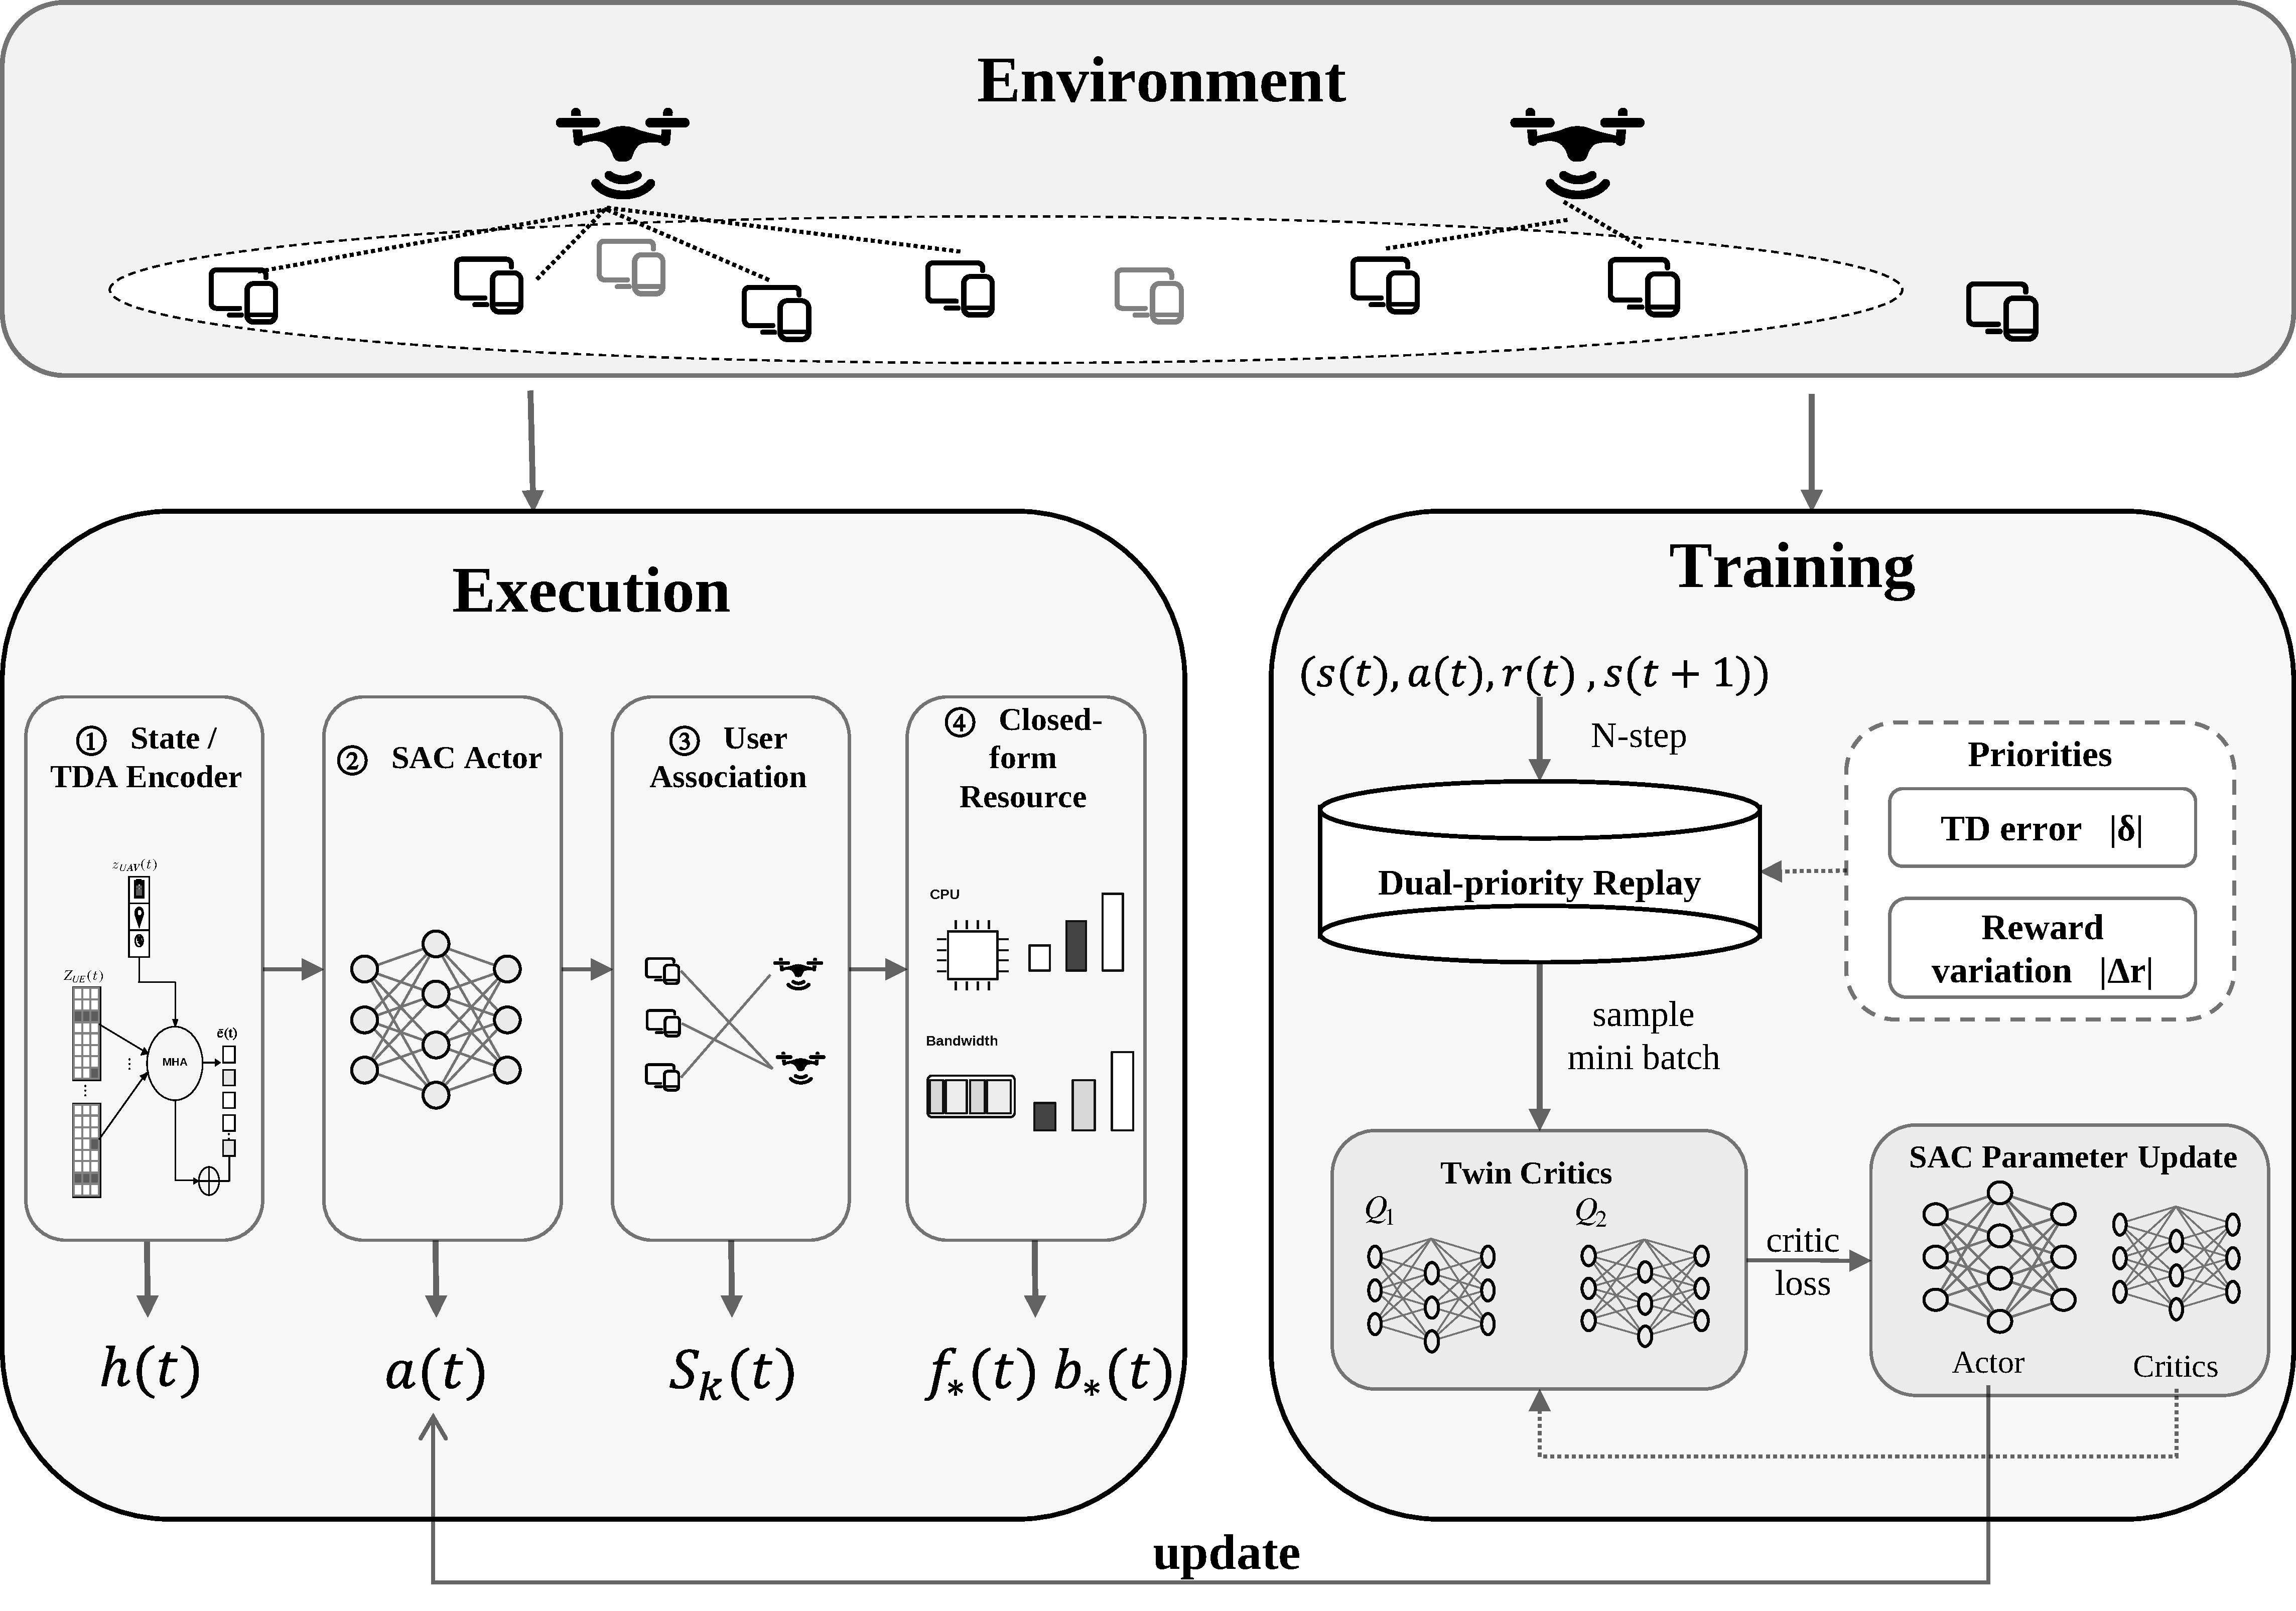
\includegraphics[width=\linewidth]{fig/frame.pdf}
\caption{Overall framework of DARS.}
\label{fig:framework}
\end{figure}


Given the outer-layer DRL outputs, including UAV trajectories $\bm{Q}$, user association $\bm{A}$, and offloading ratios $\bm{X}$, the local computation latency  $T_i^{\mathrm{loc}}(t)$ is independent of UAV-side CPU frequency and bandwidth allocation. Directly minimizing the original max-latency expression would lead to a piecewise resource allocation problem, where allocating additional edge resources to users whose edge latency is already no larger than their local latency may not further reduce the final completion latency. To keep the per-slot scheduler lightweight and analytically tractable, we solve an edge-latency-oriented inner subproblem that minimizes the computation and transmission components of the edge offloading branch. The obtained closed-form solution is optimal for the inner subproblems \textbf{P2} and \textbf{P3}, while the final task completion latency, SLRR reward, and battery evolution are still evaluated according to the original max-latency model.

\subsubsection{Computation Resource Allocation}

Let \(\omega_i(t)=x_i(t)D_i(t)\phi\) denote the offloaded computation workload of user \(i\). Define the active offloading user set as
\begin{equation}\label{eq:active_set2}
  \mathcal{S}_k^{+}(t) = \{i \in \mathcal{S}_k(t) :
  \xi_i(t) = 1 \;\text{and}\; x_i(t) > 0\},
\end{equation}
which contains users that are both task-active ($\xi_i = 1$) and have
a non-zero offloading ratio ($x_i > 0$).
For users $i \notin \mathcal{S}_k^{+}(t)$, we set $f_{i,k}(t) = 0$.
The following sub-problem is defined only over $\mathcal{S}_k^{+}(t)$,
ensuring $\omega_i(t) > 0$ for all involved users.

The computation resource allocation subproblem is formulated as \textbf{P2}:
\begin{align}\label{eq:sub_comp}
  (\textbf{P2}) \quad
  \min_{\{f_{i,k}\}} &\quad
  \sum_{i \in \mathcal{S}_k^{+}(t)} \frac{\omega_i(t)}{f_{i,k}(t)} \notag \\
  \mathrm{s.t.} &\quad
  \sum_{i \in \mathcal{S}_k^{+}(t)} f_{i,k}(t) = F_{\mathrm{UAV}},
  \; f_{i,k}(t) > 0.
\end{align}
%>> [CHANGED] Hardcoded "(18g)" replaced with \eqref{prob:P1g}.
Note that the original constraint~\eqref{prob:P1g} is an inequality
$\sum_i f_{i,k} \le F_{\mathrm{UAV}}$.
Since the objective $\omega_i / f_{i,k}$ is strictly monotonically decreasing
in $f_{i,k}$ (given $\omega_i > 0$), the capacity constraint is necessarily
tight at optimality.
Thus, replacing the inequality with an equality does not affect optimality.

\begin{theorem}[Strict Convexity]\label{thm:convex}
Sub-problem \textbf{P2} is strictly convex
over the feasible region $\{f_{i,k}>0:\sum_i f_{i,k}=F_{\mathrm{UAV}}\}$; hence,
a unique global optimum exists \cite{boyd2004convex}.
\end{theorem}
\begin{IEEEproof}
Let $n_k = |\mathcal{S}_k^{+}(t)|$ and
$\bm{f} = [f_{1,k}, \ldots, f_{n_k,k}]^{\top} \in \mathbb{R}_{++}^{n_k}$.
The Hessian matrix of the objective function
$\Psi(\bm{f}) = \sum_{i=1}^{n_k} \omega_i / f_{i,k}$ is given by
\begin{equation}\label{eq:proo}
\nabla^2 \Psi(\bm{f}) = \mathrm{diag}\!\left(\frac{2\omega_1}{f_{1,k}^3},
\frac{2\omega_2}{f_{2,k}^3}, \ldots, \frac{2\omega_{n_k}}{f_{n_k,k}^3}\right),
\end{equation}
which is positive definite since $\omega_i>0$ and $f_{i,k}>0$.
The constraint $f_{i,k} > 0$ is an open set; however, 
the feasible set $\{f_{i,k} > 0 : \sum_i f_{i,k} = F_{\mathrm{UAV}}\}$ 
is bounded. Since the objective $\omega_i / f_{i,k} \to +\infty$ 
as any $f_{i,k} \to 0^+$, the infimum cannot be attained on the 
boundary. Combined with the continuity of $\Psi(\bm{f})$ 
and the compactness of the closure 
$\{f_{i,k} \ge 0 : \sum_i f_{i,k} = F_{\mathrm{UAV}}\}$, 
the optimal solution exists in the relative interior and is 
unique by strict convexity.
\end{IEEEproof}

\begin{theorem}[Optimal Closed-Form Solution]\label{thm:closed_form}
The unique global optimum of \textbf{P2} is given by
\begin{equation}\label{eq:opt_freq}
  f_{i,k}^{*}(t) =
  F_{\mathrm{UAV}}
  \frac{\sqrt{\omega_i(t)}}
       {\sum_{j \in \mathcal{S}_k^{+}(t)} \sqrt{\omega_j(t)}},
  \quad \forall i \in \mathcal{S}_k^{+}(t).
\end{equation}
\end{theorem}

\begin{IEEEproof}
Since \(\omega_i(t)>0\) for all \(i\in\mathcal{S}_k^{+}(t)\), the objective
\(\sum_{i\in\mathcal{S}_k^{+}(t)}\omega_i(t)/f_{i,k}(t)\) is monotonically
decreasing with respect to each \(f_{i,k}(t)\). Therefore, the CPU resource
constraint must be tight at the optimum; otherwise, increasing the allocated
CPU frequency of any active offloading user can further reduce the objective.

By Theorem~\ref{thm:convex}, \textbf{P2} is strictly convex, and the KKT conditions are
sufficient for global optimality~\cite{boyd2004convex}. The Lagrangian is
\begin{equation}\label{eq:lagrangian_freq}
\mathcal{L}
=
\sum_{i\in\mathcal{S}_k^{+}(t)}
\frac{\omega_i(t)}{f_{i,k}(t)}
+
\nu
\left(
\sum_{i\in\mathcal{S}_k^{+}(t)}f_{i,k}(t)-F_{\mathrm{UAV}}
\right).
\end{equation}
where \(\nu\) is the Lagrange multiplier. From the stationarity condition,
we have
\begin{equation}\label{eq:stationarity_freq}
\frac{\partial \mathcal{L}}{\partial f_{i,k}(t)}
=
-\frac{\omega_i(t)}{f_{i,k}^2(t)}+\nu=0.
\end{equation}


Thus,
\begin{equation}\label{eq:freq_nu}
f_{i,k}(t)=\sqrt{\frac{\omega_i(t)}{\nu}}.
\end{equation}
Substituting \eqref{eq:freq_nu} into
\(\sum_{i\in\mathcal{S}_k^{+}(t)}f_{i,k}(t)=F_{\mathrm{UAV}}\), we obtain
\begin{equation}\label{eq:nu_freq}
\sqrt{\nu}
=
\frac{\sum_{j\in\mathcal{S}_k^{+}(t)}\sqrt{\omega_j(t)}}
{F_{\mathrm{UAV}}}.
\end{equation}
Since $\omega_j(t) > 0$ for all $j \in \mathcal{S}_k^+(t)$, 
it follows that $\sqrt{\nu} > 0$, i.e., the Lagrange multiplier 
$\nu > 0$.
Finally, substituting \eqref{eq:nu_freq} into \eqref{eq:freq_nu} yields
\eqref{eq:opt_freq}. Since \textbf{P2} is strictly convex, the obtained KKT point is
the unique global optimum.
\end{IEEEproof}


\subsubsection{Bandwidth Allocation}

Define the equivalent transmission workload of user~$i$ as
\begin{equation}
  \chi_{i,k}(t) = \frac{x_i(t)\,D_i(t)}
  {\log_2\!\bigl(1 + P_{\mathrm{tx}}\,g_{i,k}(t)/\sigma_n^2\bigr)}.
  \label{eq:chi}
\end{equation}
The bandwidth allocation subproblem is formulated as
\begin{align}
  (\textbf{P3})\quad \min_{\{b_{i,k}(t)\}} \quad 
  & \sum_{i \in \mathcal{S}_k^+(t)} 
    \frac{\chi_{i,k}(t)}{b_{i,k}(t)} \notag \\
  \text{s.t.} \quad 
  & \sum_{i \in \mathcal{S}_k^+(t)} b_{i,k}(t) = W, 
    \quad b_{i,k}(t) > 0.
  \label{eq:P3}
\end{align}
%
Problem \textbf{P3} is structurally identical to \textbf{P2} with $\omega_i(t)$ 
replaced by $\chi_{i,k}(t)$ and $F_{\mathrm{UAV}}$ replaced by $W$. 
By an analogous application of Theorems~\ref{thm:convex} 
and~\ref{thm:closed_form}, the unique optimal bandwidth 
allocation is
\begin{equation}\label{eq:bandwidth_opt}
    b_{i,k}^*(t) = W \cdot 
    \frac{\sqrt{\chi_{i,k}(t)}}
    {\sum_{j \in \mathcal{S}_k^+(t)} \sqrt{\chi_{j,k}(t)}}, 
    \quad \forall\, i \in \mathcal{S}_k^+(t).
\end{equation}

% ============================================================
\subsection{Outer-Layer MDP Formulation}\label{subsec:mdp}

After eliminating the instantaneous resource allocation variables, the remaining
trajectory and offloading decisions still depend on dynamic user demands and
battery evolution. A standard MLP-based policy treats all user features as a
flat vector, which may be sensitive to user ordering and may dilute the
information of active users when many users are inactive. This motivates us
to design a task-demand attention representation before applying DRL.

The inner-layer closed-form solutions eliminate the resource allocation
variables, but the remaining outer-layer problem---jointly optimizing
UAV trajectories and offloading ratios subject to stochastic task arrivals,
time-varying user distributions, and energy causality constraints---remains
a sequential decision problem under uncertainty.
Since the battery dynamics couple decisions across
time slots and the task arrival process $\xi_i(t)$ is stochastic,
neither single-slot optimization nor model-based dynamic programming
is tractable.
We therefore formulate the outer-layer problem as an MDP
and solve it via model-free DRL.

\subsubsection{MDP Formulation}

% The system is modeled as an MDP
% \(\langle \mathcal{S},\mathcal{A},\mathcal{P},\mathcal{R},\gamma\rangle\).
%>> [FIX-19] 状态/动作空间改用黑板体，与 S_k(t) 区分
The system is modeled as an MDP
\(\langle \mathbb{S},\mathbb{A},\mathcal{P},\mathcal{R},\gamma\rangle\),
where $\mathbb{S}$ and $\mathbb{A}$ are the state and action spaces,
$\mathcal{P}$ is the (unknown) transition kernel induced by the stochastic task
arrivals, user mobility and battery dynamics, $\mathcal{R}$ is the reward
function defined in~\eqref{eq:reward}, and $\gamma\in(0,1)$ is the discount
factor.

The raw state at time slot \(t\) comprises UAV states, user states,
WCT-related information, and time progress:
\begin{equation}\label{eq:state}
\bm{s}(t) = \bigl[
    \beta_k(t), \bm{q}_k(t), \tilde{\bm{\ell}}_k(t),
\bm{p}_i(t), D_i(t), \xi_i(t), t/T
\bigr].
\end{equation}
where \(\beta_k(t)\) is the normalized residual battery level of UAV \(k\),
\(\bm{q}_k(t)\in\mathbb{R}^{2}\) is the horizontal position of UAV \(k\),
\(\tilde{\bm{\ell}}_k(t)\in\mathbb{R}^{3}\) encodes the normalized
distance and two-dimensional direction from UAV \(k\) to the nearest WCT,
\(\bm{p}_i(t)\in\mathbb{R}^{2}\) is the position of user \(i\),
\(D_i(t)\) is the task data size, \(\xi_i(t)\in\{0,1\}\) is the task activation
indicator, and \(t/T\) is the normalized time progress. Therefore, the raw
state dimension is
\[
\dim(\mathbb{S}) = K(1+2+3)+M(2+1+1)+1 = 6K+4M+1.
\]



The agent outputs continuous actions including the flight direction,
speed, and proposed offloading ratio:
\begin{equation}\label{eq:action}
  \bm{a}(t) = \bigl[
    \cos\varphi_k(t),\, \sin\varphi_k(t),\, v_k(t),\, \hat{x}_i(t)
  \bigr].
\end{equation}
where $\varphi_k(t)\in[0,2\pi)$ is the flight heading angle of $u_k$, which is
represented by its cosine and sine components so as to avoid the discontinuity
at $0/2\pi$; the heading is recovered by
$\varphi_k(t)=\mathrm{atan2}\bigl(\sin\varphi_k(t),\cos\varphi_k(t)\bigr)$.
The $\tanh$ outputs of the Actor network, denoted by $a_{v,k}\in[-1,1]$ and
$a_{x,i}\in[-1,1]$, are linearly mapped to physically feasible proposals as
$v_k(t)=(a_{v,k}+1)V_{\max}/2$ and
$\hat{x}_i(t)=(a_{x,i}+1)/2$, so that
$\dim(\mathbb{A})=3K+M$.

% \begin{equation}\label{eq:action}
%   \bm{a}(t) = \Bigl[
%     \bigl\{a_{c,k}(t),\,a_{s,k}(t),\,a_{v,k}(t)\bigr\}_{k=1}^{K},\;
%     \bigl\{a_{x,i}(t)\bigr\}_{i=1}^{M}
%   \Bigr],
% \end{equation}
% where every component is a $\tanh$ output of the actor network and hence lies in
% $[-1,1]$, so that $\dim(\mathbb{A})=3K+M$. For $u_k$, the pair
% $\bigl(a_{c,k}(t),a_{s,k}(t)\bigr)$ encodes the flight heading through a
% two-component representation, which avoids the discontinuity of a scalar angle
% at $0/2\pi$. The outputs are mapped to physically feasible decisions as
% \begin{align}
% \varphi_k(t)&=\mathrm{atan2}\bigl(a_{s,k}(t),\,a_{c,k}(t)\bigr)\bmod 2\pi,
% \label{eq:heading}\\
% v_k(t)&=\tfrac{1}{2}\bigl(a_{v,k}(t)+1\bigr)V_{\max},\label{eq:speed_map}\\
% x_i(t)&=\tfrac{1}{2}\bigl(a_{x,i}(t)+1\bigr),\label{eq:offload_map}
% \end{align}
% where $\varphi_k(t)\in[0,2\pi)$ is the flight heading angle of $u_k$,
% $v_k(t)\in[0,V_{\max}]$ is its flight speed, and $x_i(t)\in[0,1]$ is the
% offloading ratio of $m_i$. The degenerate case
% $a_{c,k}(t)=a_{s,k}(t)=0$ occurs with probability zero under the stochastic
% policy and is resolved by retaining the heading of the previous slot.

% The $\tanh$ output of the Actor network is linearly mapped to
% physically feasible actions:
% $v_k(t) = (a_{v,k}+1) V_{\max}/2$ and
% $x_i(t) = (a_{x,i}+1)/2$.

%>> [FIXED] Removed the entire duplicate reward block (old lines 206--232).
%>> Kept only one clean definition with the \bar{\rho} formula integrated.
%>> Removed "soft safety barrier" and "implicit opportunity cost" phrasing.
The per-slot reward is designed to jointly reflect service latency reduction
and energy safety. Let
\begin{equation}\label{eq:active_set}
\mathcal{M}_{\mathrm{act}}(t)=
\{m_i\in\mathcal{M}\mid \xi_i(t)=1\}.
\end{equation}
denote the set of active users in the time slot \(t\). The reward is defined as
\begin{equation}\label{eq:reward}
r(t)=\sum_{m_i\in\mathcal{M}_{\mathrm{act}}(t)} \rho_i(t)
-\lambda_{\mathrm{low}}\Pi^{\mathrm{low}}(t).
\end{equation}
where the first term represents the total latency reduction achieved for active
users, and \(\lambda_{\mathrm{low}}\) controls the weight of the low-battery
penalty. The penalty term is given by
% \begin{equation}\label{eq:low_battery_penalty}
% \Pi^{\mathrm{low}}(t)=
% \sum_{u_k\in\mathcal{K}}
% \left(
% \max\{0,\epsilon-\beta_k(t)\}
% \right)^2.
% \end{equation}
% which penalizes battery levels below threshold $\varepsilon$
% and encourages timely recharging.
%>> [FIX-22] epsilon -> beta_th
\begin{equation}\label{eq:low_battery_penalty}
\Pi^{\mathrm{low}}(t)=
\sum_{u_k\in\mathcal{K}}
\left(
\max\{0,\beta_{\mathrm{th}}-\beta_k(t)\}
\right)^2,
\end{equation}
which penalizes battery levels below the safe threshold
$\beta_{\mathrm{th}}\in(0,1)$ and encourages timely recharging.

In addition, if any UAV does not have sufficient available energy to support
the current-slot net energy requirement, i.e.,
$E_k^{\mathrm{out}}(t)>B_k(t)+E_k^{\mathrm{in}}(t)$ for any $k$, the episode
terminates immediately, forfeiting all future rewards. Together, the
low-battery penalty and the terminal energy-feasibility check guide the agent
to learn a balanced service-recharging cycle.


The policy objective is to maximize the expected
discounted cumulative return:
\begin{equation}\label{eq:obj_mdp}
  \max_{\theta} \;
  \mathbb{E}_{\pi_\theta}\left[
    \sum_{t=1}^{T} \gamma^{t-1} r(t)
  \right].
\end{equation}

% \subsubsection{Task-Demand Attention Representation}\label{subsubsec:attention}

% Conventional MLP-based Actor-Critic architectures flatten all user features
% into a $4M$-dimensional vector, which suffers from two inherent deficiencies:
% (i) the flat concatenation depends on an arbitrary user ordering and thus
% lacks permutation invariance;
% (ii) under the Bernoulli task arrival model, only a subset of users are
% active at each slot, causing the critical features of a few active users
% to be diluted by the zero-valued features of many inactive users.

% To address these issues, we decompose the state vector into
% UAV-level features and per-user features:
% \begin{equation}\label{eq:decompose}
%   \bm{s}(t) \rightarrow
%   \bigl(\bm{z}_{\mathrm{UAV}}(t),\, \bm{Z}_{\mathrm{UE}}(t)\bigr),
% \end{equation}
% where $\bm{z}_{\mathrm{UAV}}(t) \in \mathbb{R}^{6K+1}$ contains
% UAV battery levels, positions, WCT information, and time progress,
% and $\bm{Z}_{\mathrm{UE}}(t) =
% [\bm{u}_1(t), \ldots, \bm{u}_M(t)]^{\top} \in \mathbb{R}^{M \times 4}$
% is the per-user feature matrix with
% $\bm{u}_i(t) = [w_{i,x}(t),\, w_{i,y}(t),\, D_i(t),\, \xi_i(t)]$.

% The per-user features are linearly projected into
% a $d_e$-dimensional embedding space:
% \begin{equation}\label{eq:proj}
%   \bm{E}_0(t) = \bm{Z}_{\mathrm{UE}}(t) \bm{W}_p,
%   \quad \bm{W}_p \in \mathbb{R}^{4 \times d_e}.
% \end{equation}
% A multi-head self-attention (MHA) module then models the
% inter-user task-demand correlations.
% %>> [CHANGED] Renamed query matrix from \bm{Q} to \bm{Q}_a
% %>> to avoid conflict with trajectory variable \bm{Q}.
% The query, key, and value matrices are computed as
% \begin{equation}\label{eq:qkv}
%   \bm{Q}_a = \bm{E}_0 \bm{W}_Q, \;\;
%   \bm{K}_a = \bm{E}_0 \bm{W}_K, \;\;
%   \bm{V}_a = \bm{E}_0 \bm{W}_V,
% \end{equation}
% where $\bm{W}_Q, \bm{W}_K, \bm{W}_V \in \mathbb{R}^{d_e \times d_e}$
% are learnable projection matrices.
% The attention output is
% \begin{equation}\label{eq:attn}
%   \bm{E}(t) = \mathrm{softmax}\!\left(
%     \frac{\bm{Q}_a\bm{K}_a^{\top}}{\sqrt{d_e / n_h}}
%   \right) \bm{V}_a,
% \end{equation}
% where the computation is independently performed across $n_h$ attention heads
% and then concatenated.
% After residual connection and layer normalization,
% mean pooling over all user embeddings yields a global
% task-demand representation:
% \begin{equation}\label{eq:pool}
%   \bar{\bm{e}}(t) = \frac{1}{M}
%   \sum_{i=1}^{M}
%   \mathrm{LN}\bigl(\bm{E}_i(t) + \bm{E}_{0,i}(t)\bigr).
% \end{equation}
% The final state representation is obtained by concatenation:
% \begin{equation}\label{eq:concat}
%   \bm{h}(t) = [\bm{z}_{\mathrm{UAV}}(t),\, \bar{\bm{e}}(t)]
%   \in \mathbb{R}^{6K+1+d_e},
% \end{equation}
% which is fed into both the Actor and Twin Critic networks. This representation is permutation-invariant with respect to 
% user ordering and adaptively adjusts attention weights according 
% to the spatio-temporal variations in task demand.

\subsubsection{Task-Demand Attention Representation}
\label{subsec:attention}

The raw state defined in \eqref{eq:state} contains \(M\) per-user feature
vectors. A standard MLP policy would flatten them into a single
\(4M\)-dimensional input, which directly mixes user-level features and does
not explicitly model the interactions among user demands. Moreover, under
the Bernoulli task arrival model, only a subset of users are active at each
slot, so the demand pattern of active users may be obscured by the features
of many inactive users. To obtain a compact representation that captures
inter-user demand correlations before aggregation, we introduce a
task-demand attention encoder before the policy head.



We split the state into UAV-level and per-user components:
\begin{equation}\label{eq:decompose}
  \bm{s}(t) \rightarrow
  \bigl(\bm{z}_{\mathrm{UAV}}(t),\, 
        \bm{Z}_{\mathrm{UE}}(t)\bigr),
\end{equation}

where $\bm{z}_{\mathrm{UAV}}(t) \in \mathbb{R}^{6K+1}$ 
concatenates the UAV-side features together with the time 
progress (from the $6K + 1$ non-user dimensions of $\mathbb{S}$), 
and $\bm{Z}_{\mathrm{UE}}(t) = 
[\bm{u}_1(t), \ldots, \bm{u}_M(t)]^{\top} 
\in \mathbb{R}^{M \times 4}$ stacks the per-user features 
$\bm{u}_i(t) = [p_{i,x}(t), p_{i,y}(t), D_i(t), \xi_i(t)]$.

% The per-user features are first projected into a 
% $d_e$-dimensional embedding space:
% \begin{equation}\label{eq:proj}
%   \bm{E}_0(t) = \bm{Z}_{\mathrm{UE}}(t) \bm{W}_p,
%   \quad \bm{W}_p \in \mathbb{R}^{4 \times d_e}.
% \end{equation}
% A multi-head self-attention (MHA) module~\cite{vaswani2017attention} with $n_h$ heads then 
% models the inter-user correlations. For each head, the query, 
% key, and value matrices are computed as
% \begin{equation}\label{eq:qkv}
%   \bm{Q}_a = \bm{E}_0 \bm{W}_Q, \;\;
%   \bm{K}_a = \bm{E}_0 \bm{W}_K, \;\;
%   \bm{V}_a = \bm{E}_0 \bm{W}_V.
% \end{equation}
% with learnable projections $\bm{W}_Q, \bm{W}_K, 
% \bm{W}_V \in \mathbb{R}^{d_e \times (d_e / n_h)}$. 
% The attention output of each head is
% \begin{equation}\label{eq:attn}
%   \bm{E}(t) = \mathrm{softmax}\!\left(
%     \frac{\bm{Q}_a\bm{K}_a^{\top}}
%          {\sqrt{d_e / n_h}}
%   \right) \bm{V}_a.
% \end{equation}
% and the outputs of all heads are concatenated to restore the 
% $d_e$-dimensional embedding. 
% After a residual connection and layer normalization, mean 
% pooling over all user embeddings yields a global demand-aware 
% representation:
% \begin{equation}\label{eq:pool}
%   \bar{\bm{e}}(t) = \frac{1}{M}
%   \sum_{i=1}^{M}
%   \mathrm{LN}\bigl(\bm{E}_i(t) + \bm{E}_{0,i}(t)\bigr).
% \end{equation}
% The final input to the Actor and Twin Critics is the 
% concatenation
% \begin{equation}\label{eq:concat}
%   \bm{h}(t) = 
%   [\bm{z}_{\mathrm{UAV}}(t),\, \bar{\bm{e}}(t)]
%   \in \mathbb{R}^{6K + 1 + d_e}.
% \end{equation}
% which is permutation-invariant with respect to user ordering 
% and adaptively re-weights users according to the spatio-temporal 
% variations in task demand.
%>> [FIX-23] Z 记号统一；[32] -> \cite{vaswani2017attention}
The per-user features are first projected into a $d_e$-dimensional embedding
space:
\begin{equation}\label{eq:proj}
\bm{Z}^{(0)}(t)=\bm{Z}_{\mathrm{UE}}(t)\bm{W}_p,\qquad
\bm{W}_p\in\mathbb{R}^{4\times d_e},
\end{equation}
where $d_e$ is the embedding dimension. A multi-head self-attention (MHA)
module~\cite{vaswani2017attention} with $n_h$ heads then models the inter-user
correlations. For the
$a$-th head ($a=1,\ldots,n_h$),
\begin{equation}
\bm Q^{(a)}=\bm Z^{(0)}\bm W^{(a)}_Q,\quad
\bm K^{(a)}=\bm Z^{(0)}\bm W^{(a)}_K,\quad
\bm V^{(a)}=\bm Z^{(0)}\bm W^{(a)}_V,
\end{equation}
with learnable projections
$\bm W^{(a)}_Q,\bm W^{(a)}_K,\bm W^{(a)}_V\in\mathbb{R}^{d_e\times(d_e/n_h)}$,
and the head output is
\begin{equation}
\bm O^{(a)}=\mathrm{softmax}\!\left(\frac{\bm Q^{(a)}(\bm K^{(a)})^{\top}}
{\sqrt{d_e/n_h}}\right)\bm V^{(a)}.
\end{equation}
The heads are concatenated and linearly mapped back to the $d_e$-dimensional
space, $\bm Z^{(1)}=\mathrm{Concat}(\bm O^{(1)},\ldots,\bm O^{(n_h)})\bm W_O$
with $\bm W_O\in\mathbb{R}^{d_e\times d_e}$. After a residual connection, layer
normalisation $\mathrm{LN}(\cdot)$ and mean pooling over all users, the global
demand-aware representation is
\begin{equation}
\bar{\bm e}(t)=\frac{1}{M}\sum_{i=1}^{M}
\mathrm{LN}\!\big(\bm Z^{(1)}_{i}(t)+\bm Z^{(0)}_{i}(t)\big),
\end{equation}
where $\bm Z^{(\cdot)}_{i}$ denotes the $i$-th row of the corresponding matrix.
The final input to the Actor and the Twin Critics is the concatenation
\begin{equation}\label{eq:concat}
\bm{h}(t)=\bigl[\bm{z}_{\mathrm{UAV}}(t),\,\bar{\bm{e}}(t)\bigr]
\in\mathbb{R}^{6K+1+d_e}.
\end{equation}
The pooled demand representation, and hence $\bm h(t)$ with respect to user
ordering, is permutation-invariant. In the Actor, $\bm h(t)$ is further
processed by two MLP layers and a fixed-dimensional linear output head that
produces the $3K$ UAV-movement components and $M$ user-indexed offloading
proposals. Therefore, the permutation invariance applies to the pooled
state representation rather than to the user-indexed action outputs.



% ============================================================
\subsection{Training Mechanisms}\label{subsec:training}
Although the attention-enhanced MDP provides a compact state representation,
training an effective policy remains challenging. The reason is that critical
events such as battery depletion, timely recharging, and hotspot switching
occur infrequently but have a significant impact on long-term performance.
If these transitions are sampled uniformly, the agent may fail to learn the
causal relationship between current service decisions and future survival.
Therefore, we combine maximum-entropy SAC~\cite{haarnoja2018soft}, dual-priority PER, and $n$-step
returns to improve exploration, emphasize informative transitions, and
accelerate reward propagation.
\subsubsection{Maximum Entropy SAC Framework}
We adopt SAC~\cite{haarnoja2018soft} as the base continuous controller.
Its objective augments the cumulative reward with an entropy bonus:
\begin{equation}\label{eq:sac_obj}
  J(\pi) = \mathbb{E}_{\pi}\left[
    \sum_{t=1}^{T} \gamma^{t-1}
    \bigl(r(t) + \alpha_{\mathrm{H}}
    \mathbb{H}(\pi(\cdot|\bm{h}(t)))\bigr)
  \right],
\end{equation}
where the entropy temperature $\alpha_{\mathrm{H}}$ is automatically
tuned via dual gradient descent.
Twin Critics with clipped double Q-learning suppress value overestimation,
and Huber loss enhances robustness against outlier TD errors.
%>> [ADDED] One sentence on delayed Actor update (matches code: ACTOR_DELAY=2).
The Actor is updated every $n_{\mathrm{act}}$ Critic steps to improve training
stability, and the target networks are soft-updated as
$\bar\psi_j\leftarrow\zeta\psi_j+(1-\zeta)\bar\psi_j$, $j=1,2$,
with $\zeta\in(0,1)$ the soft-update coefficient.
% and the target networks are soft-updated as
% $\bar\psi_j\leftarrow\varsigma\psi_j+(1-\varsigma)\bar\psi_j$, $j=1,2$,
% with $\varsigma\in(0,1)$ the soft-update coefficient.
\renewcommand{\algorithmicrequire}{\textbf{Input:}}
\renewcommand{\algorithmicensure}{\textbf{Output:}}

\begin{algorithm}[t]
\caption{DARS Training Procedure}
\label{alg:dars}
\begin{algorithmic}[1]
\REQUIRE $K, M, N_w, T, \tau, \gamma, \alpha_{\mathrm{per}},
   \beta_{\mathrm{th}},
  n, N_{\mathrm{warm}}, N_{\mathrm{batch}}, n_{\mathrm{act}}, \zeta$
\ENSURE Trained policy $\pi_\theta$
% \lambda_{\mathrm{sur}}, \lambda_{\mathrm{low}}, \beta_0,
\STATE Initialize Actor $\pi_\theta$, Twin Critics $Q_{\psi_1}, Q_{\psi_2}$,
  target networks $\bar\psi_j\!\leftarrow\!\psi_j$, entropy temperature
  $\alpha_{\mathrm{H}}$, PER buffer $\mathcal{D}$, and $n$-step buffer;

\FOR{episode $= 1, \ldots, N_{\mathrm{ep}}$}
  \STATE Reset env; $B_k(1) \leftarrow B_{\max}$; observe $\bm{s}(1)$;
  \FOR{$t = 1, \ldots, T$}
    \STATE $\bm{h}(t) \leftarrow$ encode $\bm{s}(t)$
      via the attention module;
    \STATE Sample $\bm{a}(t) \sim
      \pi_\theta(\cdot|\bm{h}(t))$;
    \STATE Execute $\bm{a}(t)$ and update UAV positions;
    \STATE $\mathcal{S}_k(t) \leftarrow$ marginal-SLRR greedy association with bounded move/swap improvement;
    \STATE $\{f_{i,k}^*, b_{i,k}^*\} \leftarrow$
      closed-form resource allocation by~\eqref{eq:opt_freq} and~\eqref{eq:bandwidth_opt};
    \STATE Observe reward $r_t$, next state $\bm{s}(t+1)$, and terminal flag $d_{\mathrm{term}}(t+1)$;
    \STATE Construct $n$-step transition $(\bm{s}_t, \bm{a}_t, G_t^{(n)},
      \bm{s}_{t+n}, d_{t+n})$ and store it into $\mathcal{D}$ with priority
      $p_z$ computed by~\eqref{eq:dual_priority};



    \IF{$|\mathcal{D}| \geq N_{\mathrm{warm}}$}
      \STATE Sample a mini-batch of size \(N_{\mathrm{batch}}\) from PER buffer $\mathcal{D}$ with IS weights;
      \STATE Update Critics via $n$-step target;
      \STATE Every $n_{\mathrm{act}}$ steps: update Actor, $\alpha_{\mathrm{H}}$, and soft-update target networks;
    \ENDIF


    \IF{$d_{\mathrm{term}}(t+1)=1$}
      \STATE \textbf{break}
    \ENDIF

  \ENDFOR
\ENDFOR
\end{algorithmic}
\end{algorithm}

\subsubsection{Dual-Priority Experience Replay}\label{subsubsec:dual_per}

Under the SLRR objective with episode termination,
battery depletion-induced termination
and hotspot rotation-induced demand shifts are both low-frequency but
high-value events.
Standard PER~\cite{schaul2016per} ranks transitions solely by
TD error $|\delta_i|$.
However, at the onset of a hotspot switch, the abrupt environmental change
has not yet propagated to the Q-value estimates,
potentially leaving TD errors small and causing critical transitions
to be undersampled.
To address this, we introduce \emph{reward variation} as a complementary
priority signal.

%>> [FIX-27] EMA 衰减 eta_r -> varrho_r（避与充电常数 eta 冲突）；样本索引 i -> z；IS 权重 w_i -> varpi_z
An exponential moving average (EMA) reward baseline $\bar{r}$ is maintained
online with decay rate $\varrho_r$:
\begin{equation}\label{eq:ema}
  \bar{r} \leftarrow \varrho_r \bar{r} + (1 - \varrho_r) r.
\end{equation}
For the $z$-th transition in the replay buffer $\mathcal{D}$, the sampling
priority is defined as
\begin{equation}\label{eq:dual_priority}
  p_z = \bigl(|\delta_z| + \epsilon\bigr)^{\alpha_{\mathrm{per}}}
  + \lambda_{\mathrm{sur}}
  \bigl(|r_z - \bar{r}| + \epsilon\bigr)^{\alpha_{\mathrm{per}}},
\end{equation}
where $\delta_z$ is the TD error, $\epsilon>0$ prevents zero priority,
$\alpha_{\mathrm{per}}\in[0,1]$ controls the priority sharpness, and
$\lambda_{\mathrm{sur}}>0$ weights the surprise term. We denote the first term
as $p_z^{\mathrm{td}}\triangleq(|\delta_z|+\epsilon)^{\alpha_{\mathrm{per}}}$
and the second as
$p_z^{\mathrm{sur}}\triangleq(|r_z-\bar{r}|+\epsilon)^{\alpha_{\mathrm{per}}}$.
The TD-error component $p_z^{\mathrm{td}}$ captures transitions with large
value estimation errors, such as near-termination critical states. The
reward-surprise component $p_z^{\mathrm{sur}}$ captures transitions whose
rewards deviate significantly from the running average, such as the SLRR spikes
or drops triggered by hotspot switches. The two components are complementary:
$p_z^{\mathrm{td}}$ responds to estimation inaccuracy, while
$p_z^{\mathrm{sur}}$ responds to environmental non-stationarity, jointly
covering both categories of rare but informative events.

The sampling probability of transition $z$ is
$\Pr(z)=p_z/\sum_{z'}p_{z'}$. To correct the bias introduced by non-uniform
sampling, the Critic loss is weighted by importance sampling (IS) weights
\begin{equation}\label{eq:is_weight}
  \varpi_z = \bigl(N_{\mathrm{buf}}\cdot \Pr(z)\bigr)^{-\beta_{\mathrm{per}}},
\end{equation}
where $N_{\mathrm{buf}}$ is the replay buffer capacity and
$\beta_{\mathrm{per}}$ is linearly annealed from $\beta_0$ to $1$. The weights
are normalized by $\max_z\varpi_z$ for numerical stability and used in the
Critic update to mitigate the bias introduced by prioritized sampling.



\subsubsection{n-Step Returns}
We extend the one-step SAC target to an \(n\)-step soft return in order to
propagate delayed service-charging consequences more efficiently. The target
is defined as
\begin{align}\label{eq:nstep}
G_t^{(n)}
={}&
\sum_{l=0}^{n-1}\gamma^l r_{t+l}
+\gamma^n(1-d_{t+n})
\Big[
\min_{j=1,2}
Q_{\bar{\psi}_j}
\bigl(\bm{h}_{t+n},\tilde{\bm{a}}_{t+n}\bigr)
\nonumber\\
&\qquad\qquad
-\alpha_{\mathrm{H}}
\log\pi_\theta
\bigl(
\tilde{\bm{a}}_{t+n}\mid\bm{h}_{t+n}
\bigr)
\Big],
\end{align}
where
$\tilde{\bm{a}}_{t+n}\sim
\pi_\theta(\cdot\mid\bm{h}_{t+n})$
and $d_{t+n}$ is the termination indicator. We use $n=3$ in all
experiments.

The multi-step accumulated real rewards reduce bootstrap bias in the
TD target, making the PER priority signal more accurate.
This is particularly beneficial for accelerating the backpropagation
of causal relationships between current service decisions
and future recharging necessity.

% ============================================================
% \subsection{Overall Algorithm and Complexity}\label{subsec:algorithm}
% To clarify how the proposed modules cooperate during training, Algorithm~\ref{alg:dars} summarizes the complete DARS procedure.
% The algorithm follows the same
% cascaded structure as Fig. 2: attention-based state encoding, SAC-based
% continuous decision-making, greedy user association, closed-form resource
% allocation, environment interaction, and prioritized replay-based network
% updates.

% At each time slot, three layers of cascaded decisions are executed:
% (i) the outer-layer Actor generates UAV motion decisions
% $(c_k, s_k, v_k)$ and offloading ratios $x_i$ from the
% attention-enhanced representation $\bm{h}(t)$
% via the reparameterization trick;
% %>> [FIXED] Hardcoded (18f) and (18e) replaced with \eqref{}.
% (ii) the middle layer performs marginal-SLRR greedy association followed
% by bounded move/swap improvement to obtain $\mathcal{S}_k(t)$, satisfying
% coverage constraint~\eqref{prob:P1f} and capacity constraint~\eqref{prob:P1e};
% (iii) the inner layer computes closed-form resource allocation
% via~\eqref{eq:opt_freq} and~\eqref{eq:opt_bw}
% with complexity $O(M)$.

% This hierarchical design compresses the DRL action dimensionality from
% $O(3K + M + 2MK)$ to $O(3K + M)$,
% and provides global optimality guarantees for the inner-layer sub-problems.





% The per-slot computational complexity consists of four components:
% (i) MHA encoding: $O(M^2 d_e)$;
% (ii) Actor forward pass: $O((6K+1+d_e) \cdot d_h)$;
% (iii) marginal-gain association: each subset-value evaluation costs $O(M)$,
% with greedy and bounded local-search candidate counts reported empirically;
% (iv) closed-form resource allocation: $O(M)$.
% During training, the dominant cost arises from Twin Critic backpropagation
% and PER SumTree updates ($O(\log|\mathcal{B}|)$ per sample).
% At inference, the single-step decision latency is on the order of milliseconds.

\begin{figure}[t]
\centering
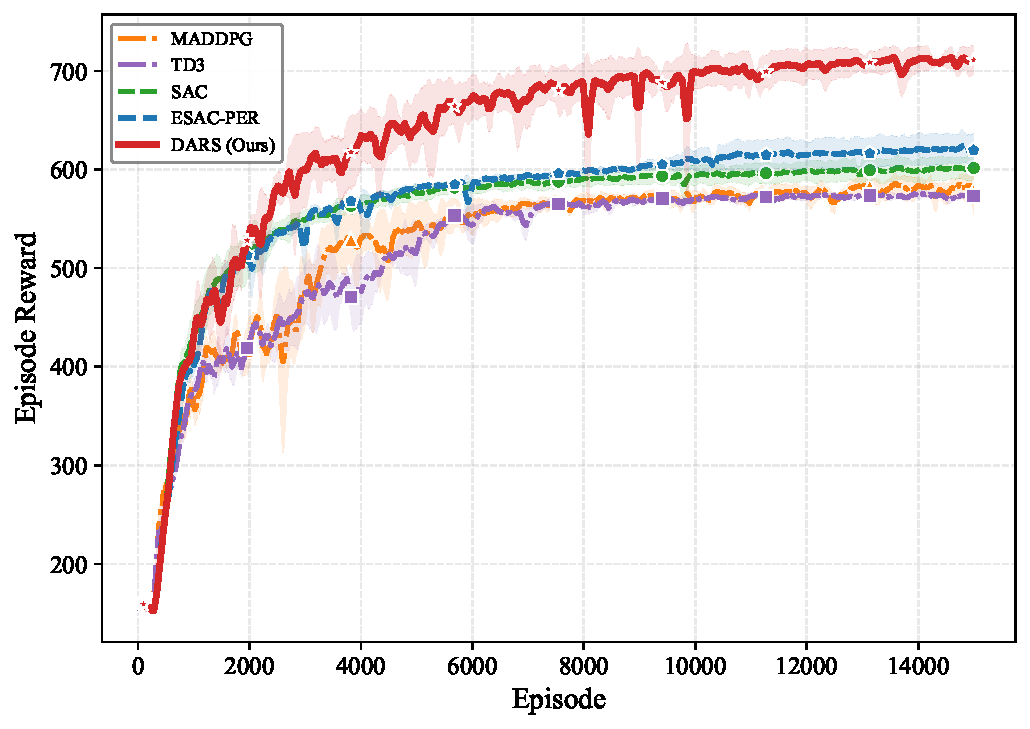
\includegraphics[width=\linewidth]{fig/new_v13_ms_multiseed_training_curves.pdf}
\caption{Training convergence of different algorithms.}
\label{fig:convergence}
\end{figure}

% \begin{figure*}[t]
% \centering
% \includegraphics[width=\linewidth]{fig_ablation_curves.pdf}
% \caption{Ablation results of DARS.}
% \label{fig:curve}
% \end{figure*}



\begin{figure*}[htbp]
    \centering
    \begin{subfigure}[b]{0.32\textwidth}
        \centering
        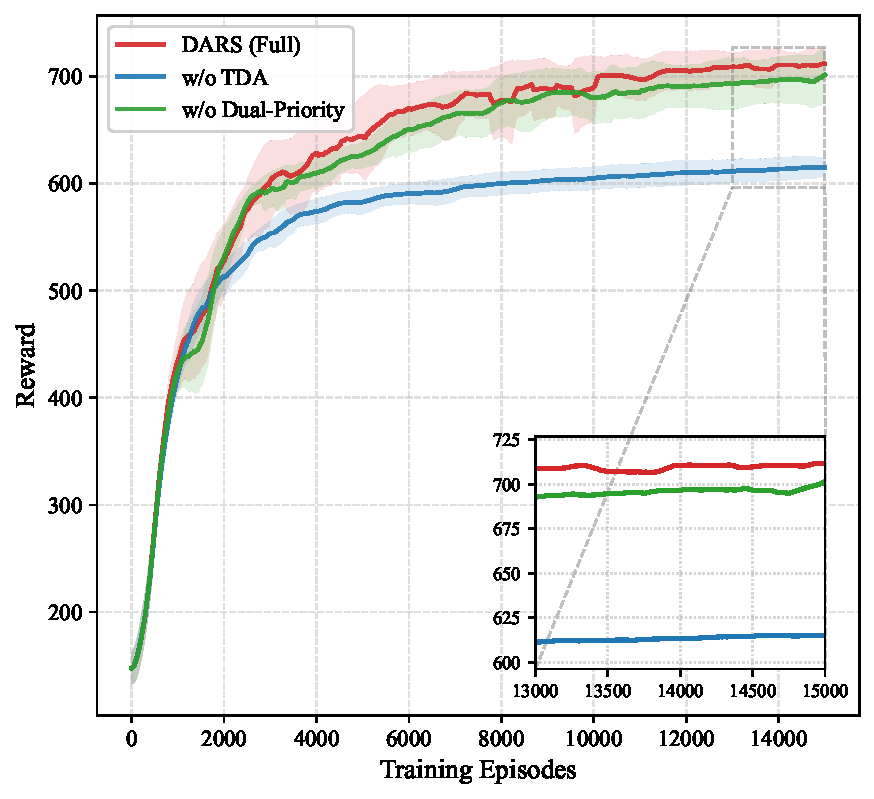
\includegraphics[width=\textwidth]{fig/fig_ablation_ep_reward.pdf}
        \caption{Training Rewards}
        \label{fig:ablation_reward}
    \end{subfigure}
    \hfill
    \begin{subfigure}[b]{0.32\textwidth}
        \centering
        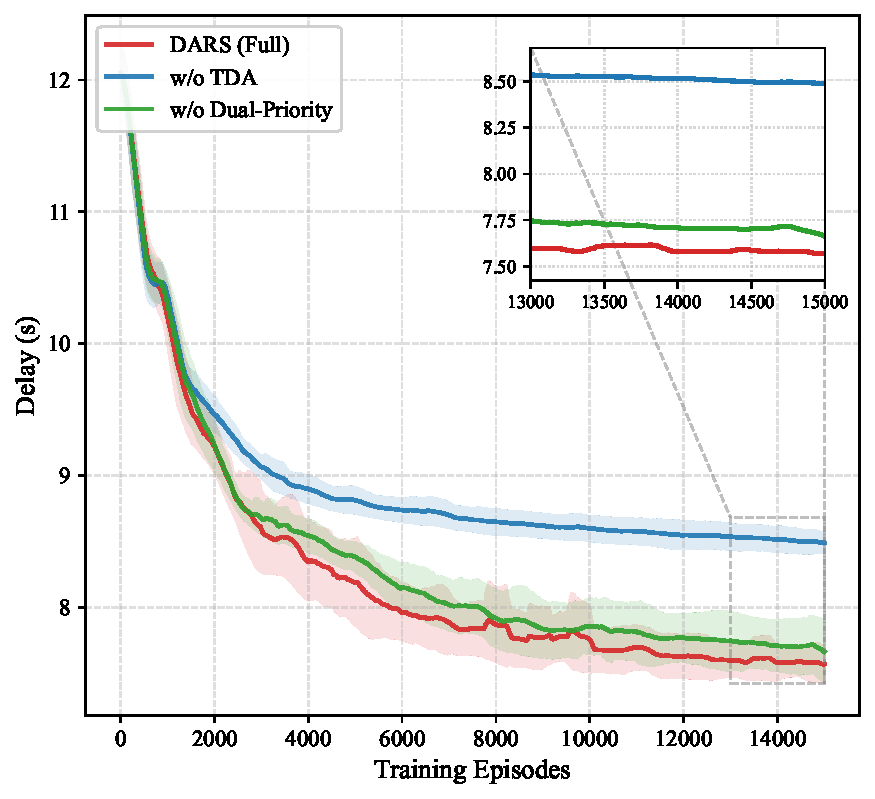
\includegraphics[width=\textwidth]{fig/fig_ablation_avg_delay.pdf}
        \caption{Average Delay}
        \label{fig:ablation_delay}
    \end{subfigure}
    \hfill
    \begin{subfigure}[b]{0.32\textwidth}
        \centering
        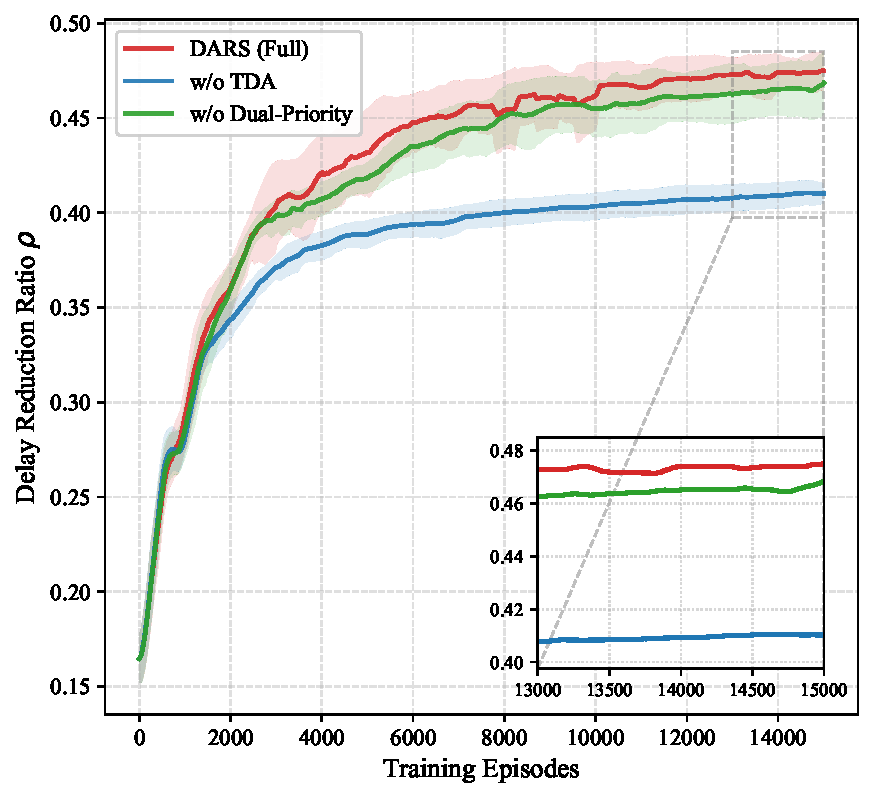
\includegraphics[width=\textwidth]{fig/fig_ablation_avg_rho.pdf}
        \caption{Delay reduction ratio}
        \label{fig:ablation_rho}
    \end{subfigure}
    \caption{Ablation study on the training performance of different modules.}
    \label{fig:ablation_curves}
\end{figure*}




\section{Simulation Results}\label{sec:experiment}
In our simulation, the task area is $500 \times 500 \,\text{m}^2$, comprising $K=2$ UAVs equipped with MEC servers, $M=30$ ground users, and $N_w =4$ wireless charging towers (WCTs). The UAVs fly at a fixed altitude of $H=100\,\text{m}$, and the WCTs are installed at a height of $70\,\text{m}$. In each time slot, every UAV jointly determines its flight direction, flight speed, and user offloading ratios. The total service horizon is divided into $50$ time slots, with each slot lasting $8\,\text{s}$. Within a time slot, the UAV flies for $1\,\text{s}$ and utilizes the remaining $7\,\text{s}$ to hover, provide offloading services, and receive wireless charging. The users are distributed according to a hotspot cluster model, where the hotspots rotate across different stages to simulate the spatio-temporal migration of task demands in urban areas. The main simulation parameters are listed in Table~\ref{tab:param}.

\begin{table}[htbp]
\centering
\caption{\textsc{System Parameter Settings}}
\label{tab:param}
\begin{tabular}{ll}
\hline
Parameter & Value \\
\hline
\hline
User transmit power $P_{\mathrm{tx}}$ & $0.1 \text{ W}$ \\
\hline
Total bandwidth $W$ & $1 \text{ MHz}$ \\
\hline
Task data size $D_i$ & $\sim \mathcal{U}(2.5, 3.0) \text{ Mbits}$ \\
\hline
Task computation intensity $\phi$ & $1000 \text{ cycles/bit}$ \\
\hline
UAV MEC computation capacity $F_{\mathrm{UAV}}$ & $3 \text{ GHz}$ \\
\hline
User local CPU frequency $f_{\mathrm{UE}}$ & $0.2 \text{ GHz}$ \\
\hline
UAV battery capacity $B_{max}$ & $40 \text{ kJ}$ \\
\hline
UAV coverage radius $R_{cov}$ & $150 \text{ m}$ \\
\hline
Maximum UAV flight speed $V_{\max}$ & $25 \text{ m/s}$ \\
\hline
WCT charging radius $L_c$ & $100 \text{ m}$ \\
\hline
Max UAV received charging power $P_{\mathrm{th}}$ & $200 \text{ W}$ \\
\hline
Actor learning rate $\alpha_a$ & $10^{-4}$ \\
\hline
Critic learning rate $\alpha_c$ & $3 \times 10^{-4}$ \\
\hline
Discount factor $\gamma$ & $0.99$ \\
\hline
Replay buffer capacity $N_{\mathrm{buf}}$ & $10^5$ \\
\hline
Batch size $N_{\mathrm{batch}}$ & $512$ \\
\hline
Total training episodes $N_{\mathrm{ep}}$ & $15000$ \\
\hline
% Number of random seeds & $3$ \\
% \hline
\end{tabular}
\end{table}
% \begin{figure*}[!t]
%     \centering
%     \includegraphics[width=1\linewidth]{fig_sens_M_1x3.pdf}
%     \caption{Performance under different user densities.}
%     \label{fig:user_density}
% \end{figure*}
\begin{figure}[t]
\centering
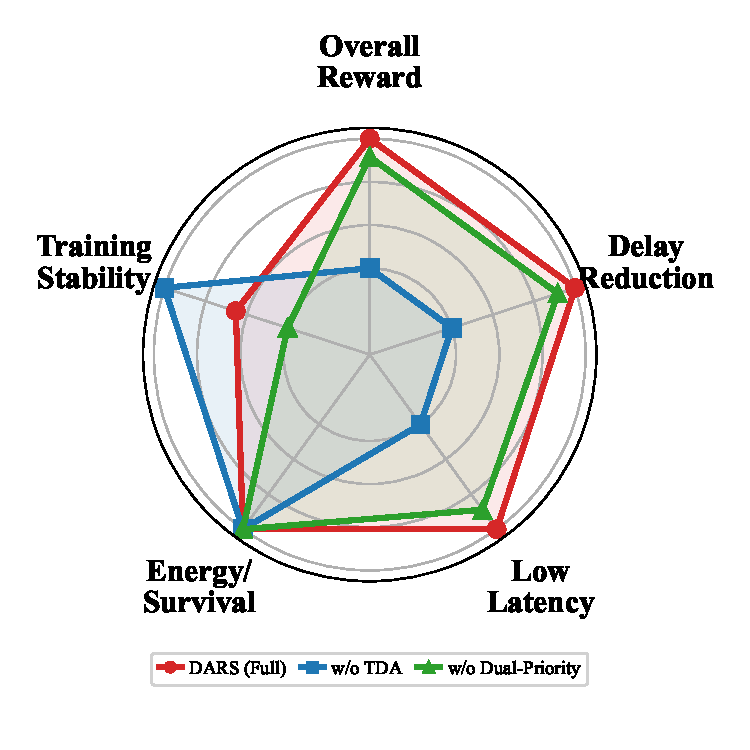
\includegraphics[width=0.6\linewidth, trim=0 20 0 15, clip]{fig/fig_ablation_radar.pdf}
\caption{Normalized multi-metric comparison.}
\label{fig:radar}
\end{figure}

\begin{figure*}[htbp]
    \centering
    \begin{subfigure}[b]{0.32\textwidth}
        \centering
        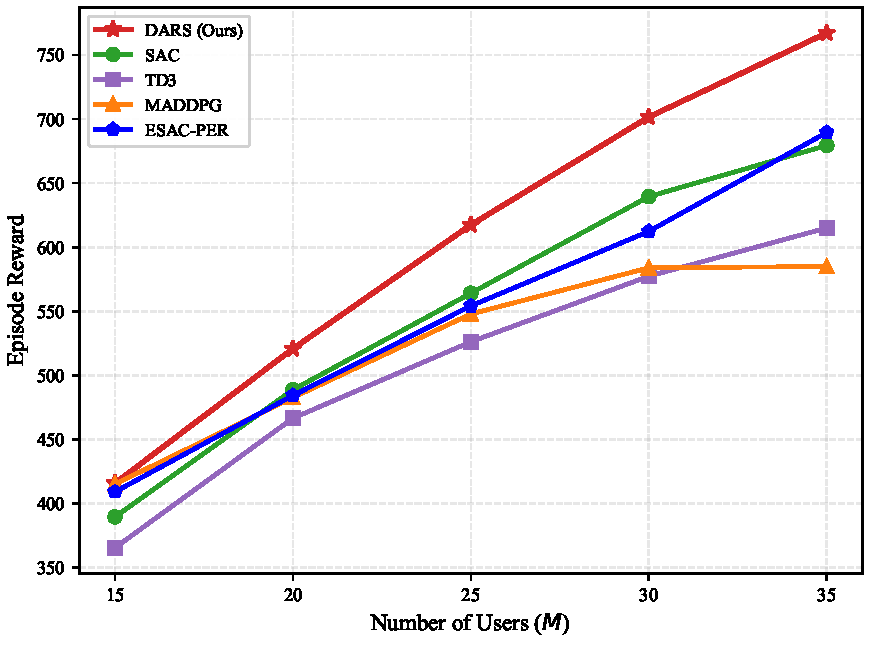
\includegraphics[width=\textwidth]{fig/fig_sens_M_reward.pdf}
        \caption{Episode Reward}
        \label{fig:sens_M_reward}
    \end{subfigure}
    \hfill
    \begin{subfigure}[b]{0.32\textwidth}
        \centering
        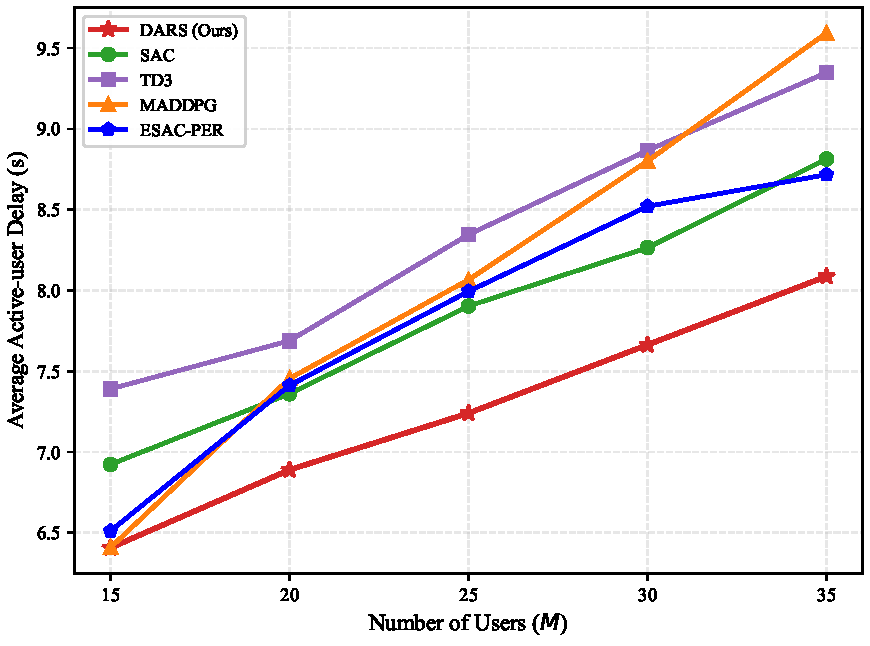
\includegraphics[width=\textwidth]{fig/fig_sens_M_delay.pdf}
        \caption{Average Delay}
        \label{fig:sens_M_delay}
    \end{subfigure}
    \hfill
    \begin{subfigure}[b]{0.32\textwidth}
        \centering
        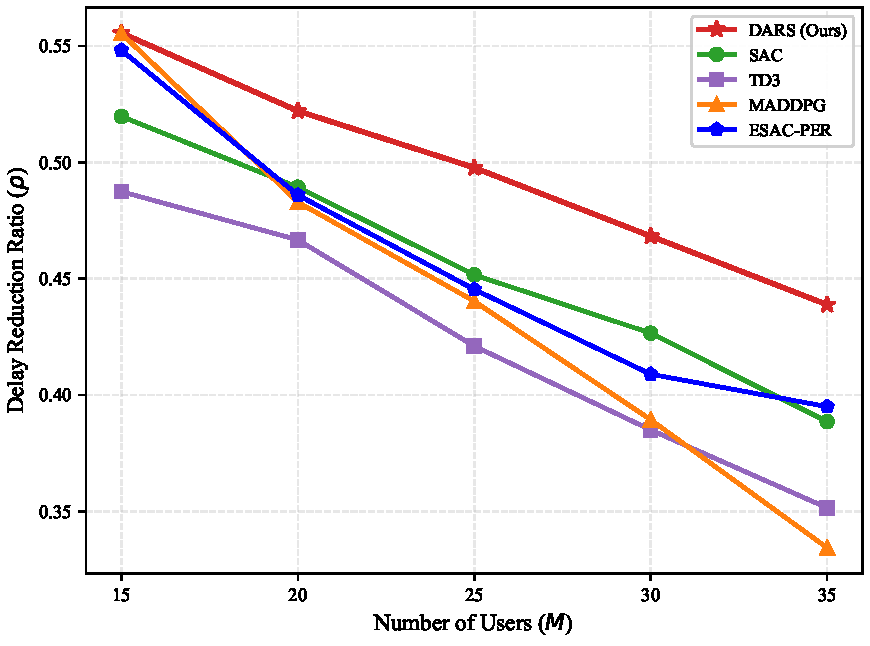
\includegraphics[width=\textwidth]{fig/fig_sens_M_rho.pdf}
        \caption{Delay reduction ratio}
        \label{fig:sens_M_rho}
    \end{subfigure}
    \caption{Performance under different user densities.}
    \label{fig:sens_M_combined}
\end{figure*}

\begin{figure*}[htbp]
    \centering
    \begin{subfigure}[b]{0.32\textwidth}
        \centering
        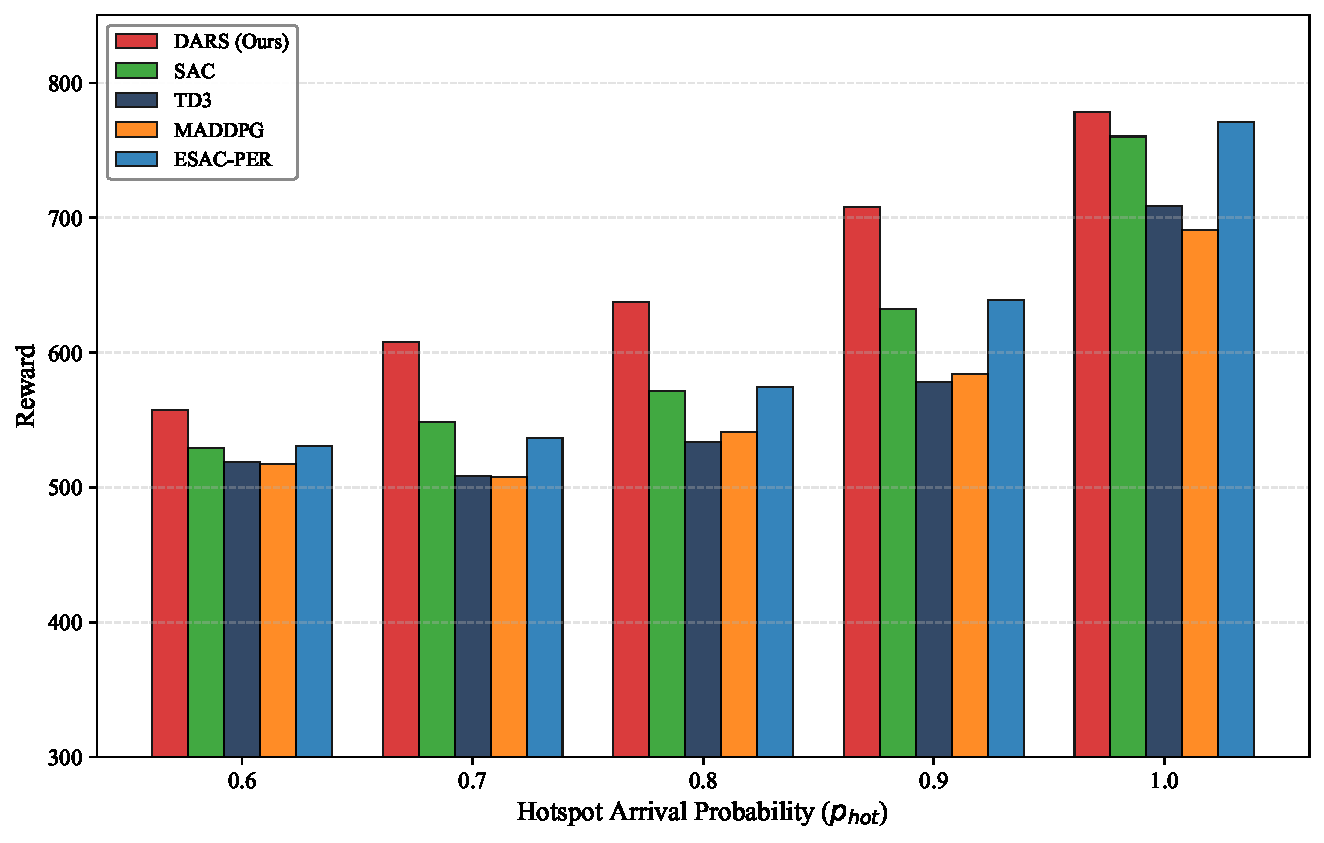
\includegraphics[width=\textwidth]{fig/fig_hot_bar_reward.pdf}
        \caption{Evaluation Reward}
        \label{fig:hot_bar_reward}
    \end{subfigure}
    \hfill
    \begin{subfigure}[b]{0.32\textwidth}
        \centering
        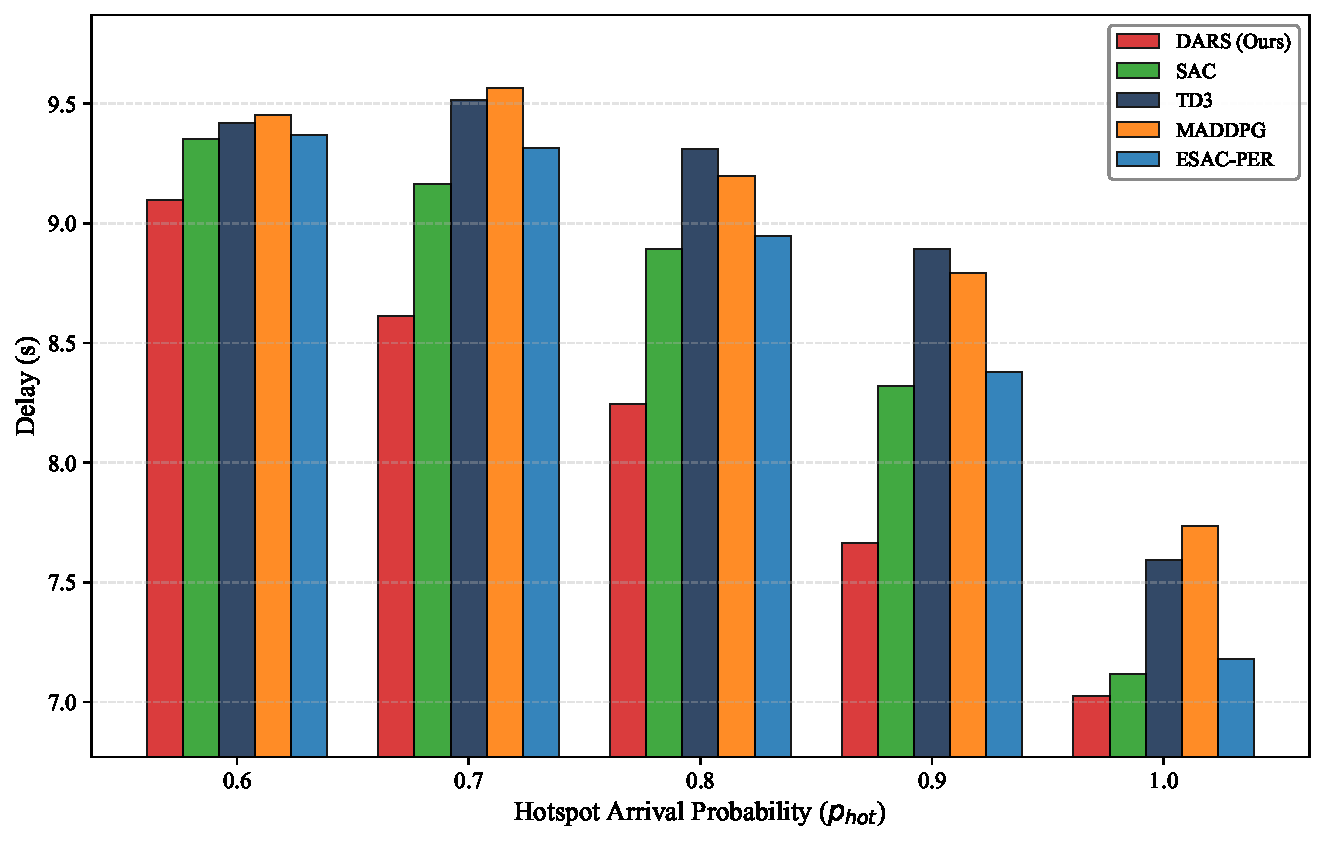
\includegraphics[width=\textwidth]{fig/fig_hot_bar_delay.pdf}
        \caption{Average Delay}
        \label{fig:hot_bar_delay}
    \end{subfigure}
    \hfill
    \begin{subfigure}[b]{0.32\textwidth}
        \centering
        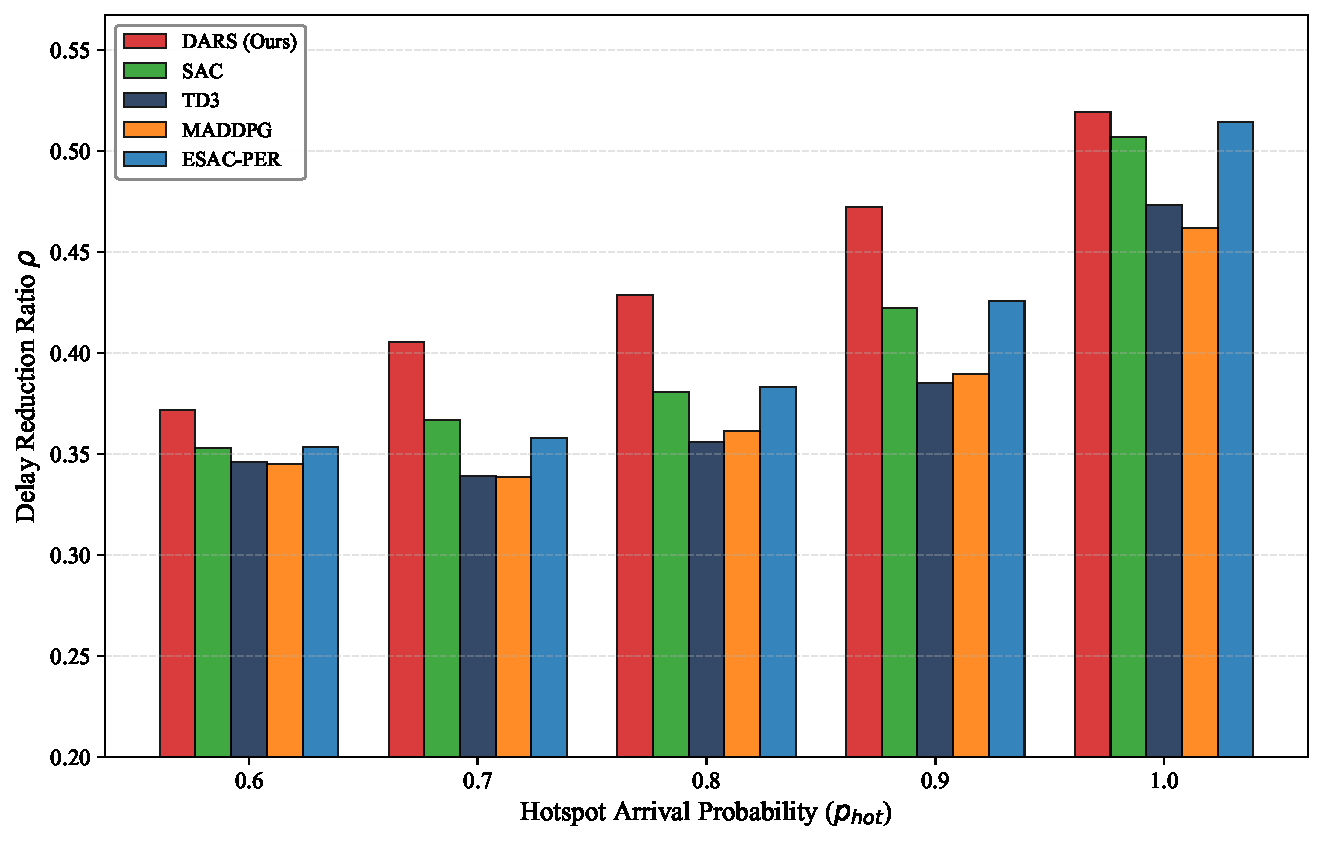
\includegraphics[width=\textwidth]{fig/fig_hot_bar_rho.pdf}
        \caption{Delay reduction ratio}
        \label{fig:hot_bar_rho}
    \end{subfigure}
    \caption{Performance under different hotspot intensities.}
    \label{fig:hot_bar_combined}
\end{figure*}



\subsection{Baseline Algorithms}
For a fair comparison, all baseline methods are evaluated under the identical environment, state/action spaces, reward function, and training budget as the proposed DARS, differing only in their policy representations and learning mechanisms.


\begin{itemize}
%\item \textbf{DARS} : A hybrid optimization architecture that couples a TDA-enhanced SAC policy and Dual-Priority PER for efficient continuous control with an exact closed-form analytical solution for resource scheduling.
\item \textbf{ESAC-PER}~\cite{nabi2025jour}: An enhanced SAC baseline incorporating double critics,
standard TD-error PER, and automatic temperature tuning, without the attention
mechanism and the dual-priority ranking.

\item \textbf{SAC}~\cite{haarnoja2018soft,chen2023sac_mec}: Standard maximum entropy SAC without TDA and PER, where states are encoded via a multi-layer perceptron (MLP).
\item \textbf{TD3}~\cite{fujimoto2018td3}: Twin Delayed Deep Deterministic Policy Gradient method, employing a deterministic policy and double critics.
\item \textbf{MADDPG}~\cite{lowe2017multi}: Multi-Agent DDPG adopting the centralized training with decentralized execution (CTDE) paradigm, where each UAV possesses an independent actor.
\end{itemize}

% 替换
The experiments adopt three performance metrics: (1) \emph{Reward}, i.e., the
cumulative SLRR; (2) \emph{Average SLRR} $\rho$; and (3) \emph{Average Delay}.
All baselines share the same inner-layer closed-form allocation in (\ref{eq:opt_freq}) and (\ref{eq:bandwidth_opt}),
so that the comparison isolates the effect of the outer-layer policy
representation and the replay mechanism.

\subsection{User Association Evaluation}
We separately evaluate the association layer on 50 independently generated
snapshots with $K=2$, $M=14$, and $N_{\max}=5$, using the channel and current
resource-allocation models of the simulator. For each snapshot, the Actor
offloading ratios are sampled once and kept fixed across methods. Each user
can be assigned to UAV 1, UAV 2, or remain unassociated, giving
$3^{14}=4{,}782{,}969$ possible assignments before feasibility pruning. The
exact reference is computed by precomputing each UAV's values for all
$2^{14}$ user subsets and combining disjoint subsets with a subset dynamic
program. Table~\ref{tab:association_quality} reports each method's objective
as a fraction of this exact reference and its mean association time.

\begin{table}[t]
\centering
\caption{Association objective and computation time on 50 small instances.}
\label{tab:association_quality}
\begin{tabular}{lccc}
\hline
Method & Mean / worst ratio & Mean time (ms) \\
\hline
Distance-priority greedy & 91.88\% / 80.21\% & 0.056 \\
Marginal-gain greedy & 99.12\% / 92.26\% & 1.615 \\
Marginal gain + 2 move/swap passes & 99.37\% / 92.26\% & 1.998 \\
Exact subset-DP reference & 100\% / 100\% & 14.942 \\
\hline
\end{tabular}
\end{table}

The timing measurements were obtained on Windows 11 with an Intel Core
i9-14900HX processor and Python 3.13.9. The subset-value precomputation takes
14.530~ms on average, while combining the values takes 0.412~ms. In a separate
dense-overlap stress case with all
$M=30$ users active, marginal greedy with two move/swap passes takes 17.267~ms
on average (23.057~ms maximum over 100 repetitions). These timings are
implementation measurements for the stated simulator setup. The local search
improves the sampled mean objective from 99.12\% to 99.37\% of the exact
reference; the empirical worst case remains 92.26\%. Since the set objective
used by the implemented allocator has not been proved submodular, these
results are empirical and do not imply a worst-case approximation guarantee.



\subsection{Convergence Analysis}

 We present the training convergence curves of different algorithms in Fig.~\ref{fig:convergence}. We evaluated all algorithms under the default environmental setting ($M=30$, $K=2$, $p_{\mathrm{hot}}=0.5$) and trained them over 15,000 episodes to ensure full convergence. At the end of training, DARS significantly achieves improvements of 13.3\%, 19.3\%, 24.7\%, and 25.8\% compared to ESAC-PER, SAC, TD3, and MADDPG, respectively, as shown in Fig.~\ref{fig:convergence} . Besides, we see that DARS not only attains the highest final performance but also converges faster and more stably than the baseline algorithms from Fig.~\ref{fig:convergence}. This is because the proposed task-demand-aware state representation allows the UAVs to quickly grasp the urgency of ground users, while the dual-priority experience replay mechanism prioritizes learning from highly informative transition samples, thereby significantly accelerating the training process and preventing the policy from falling into local optima.

\subsection{Ablation Study}
To quantify the contribution of the proposed components, we construct two variants by independently removing the Task-Demand Attention  module and the dual-priority replay mechanism while keeping all other settings unchanged. The results are averaged over the final 500 training episodes across three independent seeds. As shown in Fig.~\ref{fig:ablation_curves}, the complete DARS achieves a steady-state reward of 
$710.46\pm11.19$, an SLRR of $0.4740\pm0.0077$, and an average delay of $7.5809\pm0.1108$~s. Compared with DARS without TDA, the complete model improves the reward by 15.56\%, increases the SLRR by 6.36 percentage points, and reduces the average delay by 10.79\%. These results confirm that TDA is primarily responsible for extracting demand-dependent spatial and temporal features. Compared with DARS without dual-priority replay, the complete model improves the reward by 2.22\% and reduces the delay by 1.76\%. Moreover, removing dual-priority replay increases the reward deviation from 11.19 to 22.25, indicating that prioritizing demand-shift and energy-critical transitions improves post-convergence stability.
Fig.~\ref{fig:radar} provides a complementary visualization based on the final 50 evaluation episodes. All variants complete the entire 50-slot horizon without battery depletion; therefore, the energy-survival dimension is saturated and does not distinguish the three variants.
\subsection{Scalability Analysis}


\subsubsection{Impact of the Number of Users}
We present the impact of user density in Fig.~\ref{fig:sens_M_combined}. We fixed the number of UAVs $K=2$ and the hotspot arrival probability $p_{\mathrm{hot}}=0.5$, while we change the number of ground users $M$ from 15 to 35 with a step size of 5.

\textit{a) Episode reward:}
On average, DARS achieves improvements of 9.28\%, 9.07\%, 17.79\%, and 14.40\% compared to ESAC-PER, SAC, TD3, and MADDPG, respectively, as shown in Fig.~\ref{fig:sens_M_reward}. Besides, Fig.~\ref{fig:sens_M_reward} shows that the episode reward generally increases as $M$ grows. Since the episode reward aggregates the latency-reduction contributions of active users, its absolute value can increase with $M$ even though the competition for limited computation and communication resources becomes stronger.


\textit{b) Average delay:}
On average, DARS achieves reductions of 7.07\%, 7.55\%, 12.80\%, and 9.30\% compared to ESAC-PER, SAC, TD3, and MADDPG, respectively, as shown in Fig.~\ref{fig:sens_M_delay}. Meanwhile, Fig.~\ref{fig:sens_M_delay} shows a similar trend as the user density increases, the average delay of each algorithm gradually climbs. This trend is also attributed to the increased system load, which intensifies the competition for finite computation and
bandwidth resources and consequently increases the average
active-user completion latency. These results highlight DARS’s effectiveness in alleviating congestion and improving service timeliness.

\textit{c) Delay reduction ratio:} 
On average, DARS significantly improves 9.23\%, 9.30\%, 18.11\%, and 14.54\% over ESAC-PER, SAC, TD3, and MADDPG, respectively, as shown in Fig.~\ref{fig:sens_M_rho}. We can see from Fig.~\ref{fig:sens_M_rho}, DARS consistently outperforms all other baselines for any $M$. This demonstrates that DARS is more effective at optimizing UAV trajectories and offloading policies under different system loads, thereby achieving a more robust trade-off among resource allocation and user demand satisfaction.

% \begin{figure*}[t]
% \centering
% \includegraphics[width=1\linewidth]{fig_trajectory_M25.pdf}
% \caption{UAV trajectories.}
% \label{fig:trajectory}
% \end{figure*}



\subsubsection{Impact of the Number of Hotspot Intensities}
Next, we present the impact of hotspot intensity in Fig.~\ref{fig:hot_bar_combined}. We fixed the number of UAVs $K=2$ and the number of users $M=30$, while we change the hotspot arrival probability $p_{\mathrm{hot}}$ from $0.6$ to
$1.0$ with a step size of $0.1$, while keeping $p_{\mathrm{cold}}$ fixed.


\textit{a) Evaluation reward:} 
On average, DARS achieves improvements of 0.97\%, 2.40\%, 9.85\%, and 12.65\% compared to ESAC-PER, SAC, TD3, and MADDPG, respectively, as shown in Fig.~\ref{fig:hot_bar_reward}. Besides, we see that all algorithms generally increase their rewards with increasing $p_{\mathrm{hot}}$ up to $p_{\mathrm{hot}}=0.9$ from Fig.~\ref{fig:hot_bar_reward}. This is because a higher $p_{\mathrm{hot}}$ increases the task activation probability within the designated hotspot clusters, making active demands more spatially concentrated in these regions and allowing UAVs to serve multiple active users more efficiently.
\emph{b) Average delay:} On average, DARS significantly achieves reductions of 2.18\%, 1.32\%, 7.48\%, and 9.20\% over ESAC-PER, SAC, TD3, and MADDPG, respectively, as shown in Fig.~\ref{fig:hot_bar_delay}. We can see from Fig.~\ref{fig:hot_bar_delay}, DARS consistently outperforms all other baselines across various $p_{\mathrm{hot}}$. This demonstrates that DARS is more resilient to dynamic spatial demand distributions, leveraging its task-demand-aware representation to prioritize the most urgent requests in heavily congested areas.
\emph{c) Delay reduction ratio:} On average, DARS achieves improvements of 0.96\%, 2.46\%, 9.77\%, and 12.43\% compared to ESAC-PER, SAC, TD3, and MADDPG, respectively, as shown in Fig.~\ref{fig:hot_bar_rho}. Meanwhile, Fig.~\ref{fig:hot_bar_rho} further shows that DARS maintains
the best SLRR performance across the tested hotspot intensities,
demonstrating its robustness to different levels of spatially
concentrated task arrivals.

\begin{figure*}[htbp]
    \centering
    \begin{subfigure}[b]{0.32\textwidth}
        \centering
        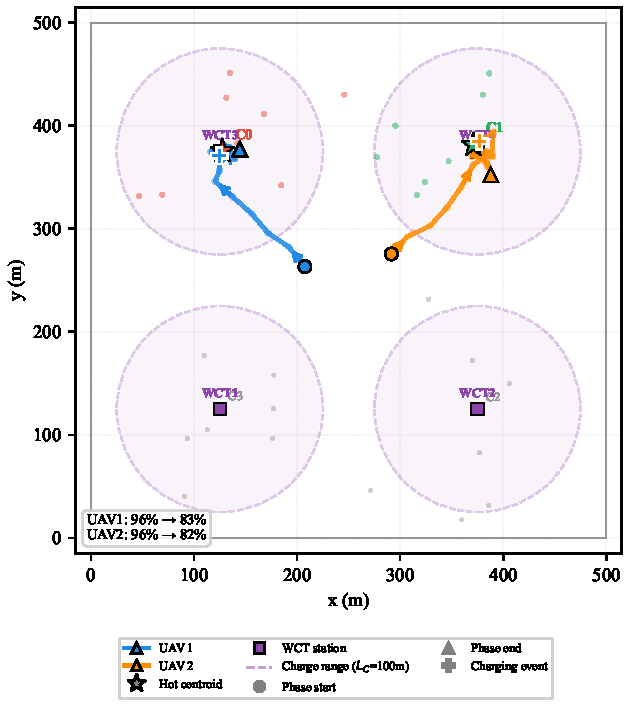
\includegraphics[
            width=\textwidth,
            height=4cm,
            keepaspectratio
        ]{fig/fig_trajectory_M25_phase1.pdf}
        \caption{Phase I}
        \label{fig:traj_phase1}
    \end{subfigure}
    \hfill
    \begin{subfigure}[b]{0.32\textwidth}
        \centering
        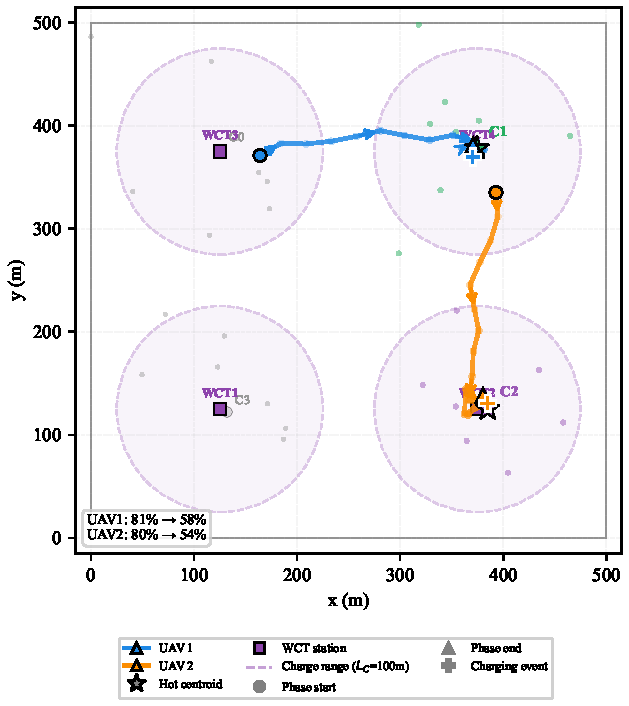
\includegraphics[
            width=\textwidth,
            height=4cm,
            keepaspectratio
        ]{fig/fig_trajectory_M25_phase2.pdf}
        \caption{Phase II}
        \label{fig:traj_phase2}
    \end{subfigure}
    \hfill
    \begin{subfigure}[b]{0.32\textwidth}
        \centering
        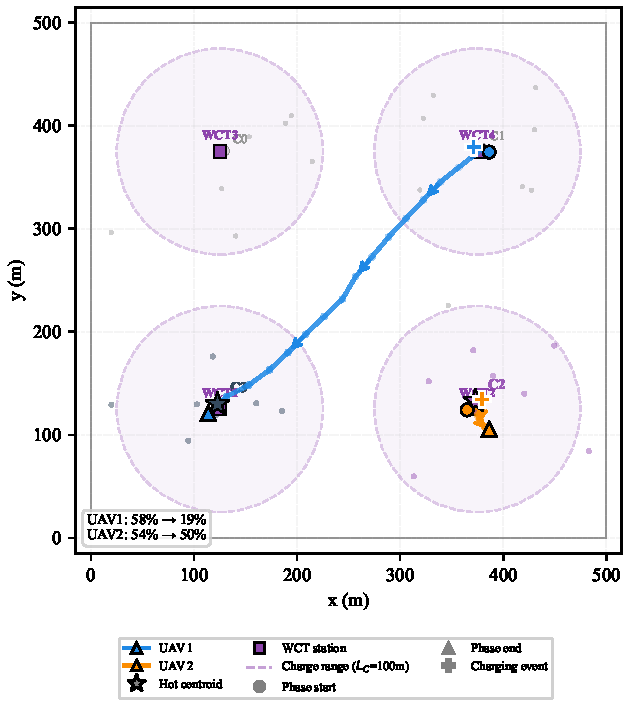
\includegraphics[
            width=\textwidth,
            height=4cm,
            keepaspectratio
        ]{fig/fig_trajectory_M25_phase3.pdf}
        \caption{Phase III}
        \label{fig:traj_phase3}
    \end{subfigure}
    \caption{UAV trajectories.}
    \label{fig:trajectory}
\end{figure*}



% \begin{figure*}[t]
% \centering
% \includegraphics[width=1\linewidth]{fig_attention_heatmap.pdf}
% \caption{Spatial Distributions of Received Self-Attention Scores During Hotspot Migration.}
% \label{fig:heatmap}
% \end{figure*}



% Fig.~\ref{fig:hotspot} presents the comparison under different hotspot arrival probabilities $p_{\mathrm{hot}} \in \{0.6, 0.7, 0.8, 0.9, 1.0\}$. On average, DARS improves upon SAC by 12.4\%, TD3 by 17.5\%, MADDPG by 16.5\%, and ESAC-PER by 9.8\%. The superiority is most pronounced under moderate hotspot intensities ($p_{\mathrm{hot}} \in [0.7, 0.9]$): at $p_{\mathrm{hot}} = 0.8$, DARS achieves $\rho = 0.445$, outperforming TD3 by 28.5\%, MADDPG by 19.4\%, SAC by 18.8\%, and ESAC-PER by 14.3\%. Under the extreme case of $p_{\mathrm{hot}} = 1.0$, ESAC-PER performs comparably to DARS (0.522 versus 0.517, with a marginal gap of 0.9\%), which is the only setting where DARS does not secure an absolute lead.
\subsection{Policy Behavior Under Dynamic Hotspots}




\subsubsection{Trajectory and Charging Behavior}

Fig.~\ref{fig:trajectory} illustrates the UAV trajectories and battery evolution during one
representative 50-slot evaluation episode with random seed 43 and without
exploration noise.
During Phase~I ($t=0$--$15$), clusters $\mathcal{C}_0$ and $\mathcal{C}_1$ are
designated as hotspots; the hotspot set rotates to
$\{\mathcal{C}_1,\mathcal{C}_2\}$ in Phase~II ($t=16$--$31$) and to
$\{\mathcal{C}_2,\mathcal{C}_3\}$ in Phase~III ($t=32$--$49$).
The UAVs
accordingly redirect their trajectories toward the newly activated regions while
retaining access to nearby WCTs. As annotated in Fig.~\ref{fig:trajectory}, the battery levels of $u_1$ and $u_2$ decrease from 96\%
to 83\% and from 96\% to 82\% in Phase~I, from 81\% to 58\% and from 80\% to
54\% in Phase~II, and from 58\% to 19\% and from 54\% to 50\% in Phase~III.
The charging events marked in Fig.~\ref{fig:trajectory} show that both UAVs repeatedly traverse the
coverage of the WCTs while migrating between hotspots, so that the net battery
depletion over each phase is far smaller than the energy that would be consumed
by continuous flight and hovering alone. In particular, $u_2$ loses only 4
percentage points over the whole of Phase~III while remaining in service,
indicating that DARS coordinates demand-responsive service with preventive
energy replenishment rather than greedily remaining near active users until
battery depletion.
\begin{figure*}[htbp]
    \centering
    \begin{subfigure}[b]{0.32\textwidth}
        \centering
        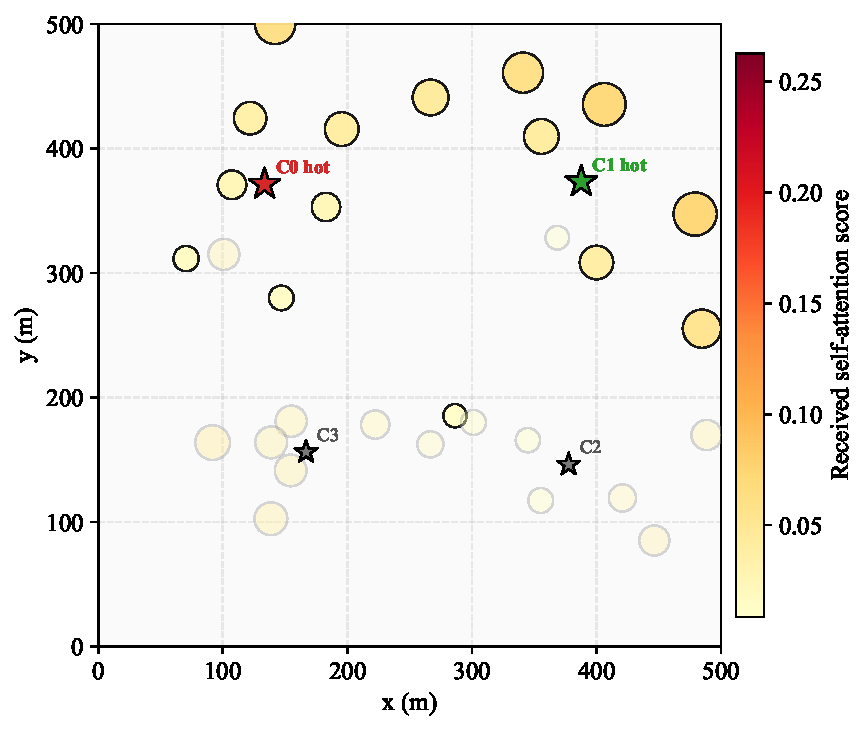
\includegraphics[width=\textwidth,            height=3cm,
            keepaspectratio]{fig/fig_attention_heatmap_step14.pdf}
        \caption{Phase I ($t=14$)}
        \label{fig:attn_phase1}
    \end{subfigure}
    \hfill
    \begin{subfigure}[b]{0.32\textwidth}
        \centering
        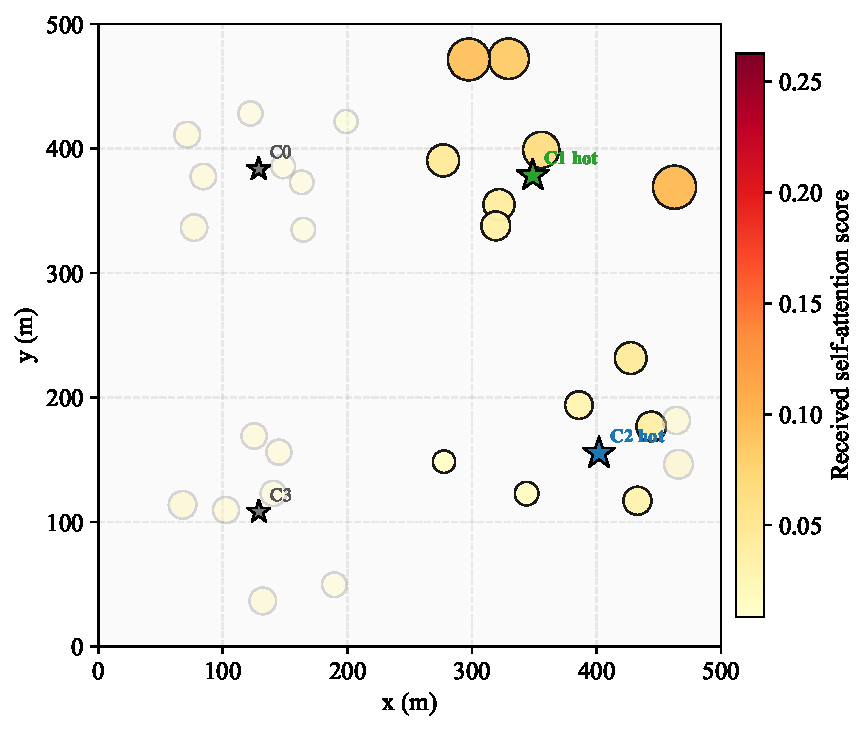
\includegraphics[width=\textwidth,            height=3cm,
            keepaspectratio]{fig/fig_attention_heatmap_step18.pdf}
        \caption{Phase II ($t=18$)}
        \label{fig:attn_phase2}
    \end{subfigure}
    \hfill
    \begin{subfigure}[b]{0.32\textwidth}
        \centering
        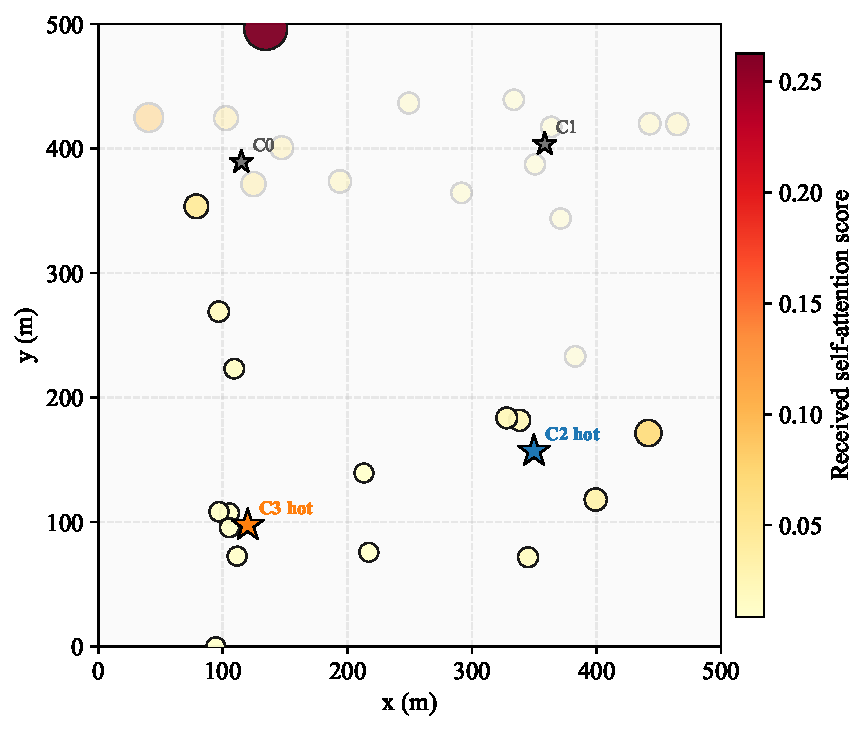
\includegraphics[width=\textwidth,            height=3cm,
            keepaspectratio]{fig/fig_attention_heatmap_step35.pdf}
        \caption{Phase III ($t=35$)}
        \label{fig:attn_phase3}
    \end{subfigure}
    \caption{Spatial distributions of received self-attention scores during hotspot migration.}
    \label{fig:attention_heatmaps}
\end{figure*}
\subsubsection{Spatial Attention Adaptation}
To qualitatively examine how the TDA module responds to dynamic
traffic demands, Fig.~\ref{fig:attention_heatmaps} visualizes
the spatial distributions of the received self-attention scores at
three representative time slots. The results are obtained from one
50-slot evaluation episode with random seed 43 and without exploration
noise. For each UE, its received attention score is calculated by
averaging the attention weights assigned to it over all query UEs and
attention heads in the actor network. The resulting scores are
normalized across all UEs for visualization. Both marker color and
area represent the normalized attention score, with darker and larger
markers indicating higher attention. Dark-edged markers denote active
UEs, whereas stars indicate the centroids of the current hotspot
clusters.

As shown in Fig.~\ref{fig:attn_phase1}, at $t=14$,
%>> [FIX-33] $C_0$/$C_1$/$C_2$/$C_3$ -> $\mathcal{C}_0$ 等（共6处）
relatively high attention scores are mainly observed around $\mathcal{C}_0$
and $\mathcal{C}_1$, which are the hotspot clusters in Phase~I. After the first
hotspot transition, the high-attention region shifts toward $\mathcal{C}_1$
and $\mathcal{C}_2$ at $t=18$, as illustrated in
Fig.~\ref{fig:attn_phase2}. This redistribution shows
that the learned attention pattern adapts to the change in the spatial
distribution of active tasks. At $t=35$,as illustrated in
Fig.~\ref{fig:attn_phase3}, the UEs receiving relatively
high attention are primarily located around $\mathcal{C}_2$ and $\mathcal{C}_3$, following
the second hotspot migration.

Overall, the attention distribution evolves consistently with the
spatial migration of traffic hotspots. This result provides a
qualitative interpretation of how TDA captures time-varying demand
patterns and adjusts the policy representation accordingly. The
performance benefit of TDA is further supported by the quantitative
ablation results in Fig.~\ref{fig:ablation_curves}.

\section{Conclusion}

This paper investigates the joint optimization of UAV trajectories, task offloading, and resource allocation to maximize the service latency reduction ratio in multi-UAV-assisted MEC systems with WCT-enabled wireless charging. To tackle the sparse reward dilemma induced by energy depletion, we propose a hierarchical task-demand-aware reinforcement learning framework, called DARS. In the outer layer, a SAC policy embedded with multi-head self-attention jointly determines the continuous trajectories and offloading ratios. In the inner layer, square-root proportional closed-form solutions for computation frequency and bandwidth allocation are derived via the KKT conditions. Furthermore, dual-priority PER and $n$-step returns are combined to reinforce the learning of critical terminal transitions. Simulation results demonstrate that DARS outperforms existing baselines in
terms of cumulative reward, average latency reduction ratio, and task
completion latency.






% if have a single appendix:
%\appendix[Proof of the Zonklar Equations]
% or
%\appendix  % for no appendix heading
% do not use \section anymore after \appendix, only \section*
% is possibly needed

% use appendices with more than one appendix
% then use \section to start each appendix
% you must declare a \section before using any
% \subsection or using \label (\appendices by itself
% starts a section numbered zero.)
%




% trigger a \newpage just before the given reference
% number - used to balance the columns on the last page
% adjust value as needed - may need to be readjusted if
% the document is modified later
%\IEEEtriggeratref{8}
% The "triggered" command can be changed if desired:
%\IEEEtriggercmd{\enlargethispage{-5in}}

% references section

% can use a bibliography generated by BibTeX as a .bbl file
% BibTeX documentation can be easily obtained at:
% The IEEEtran BibTeX style support page is at:
% http://www.michaelshell.org/tex/ieeetran/bibtex/
%\bibliographystyle{IEEEtran}
% argument is your BibTeX string definitions and bibliography database(s)
%\bibliography{IEEEabrv,../bib/paper}
%
% <OR> manually copy in the resultant .bbl file
% set second argument of \begin to the number of references
% (used to reserve space for the reference number labels box)

\bibliographystyle{IEEEtran}
\bibliography{references}


% \begin{thebibliography}{20}
% \bibitem{wang2023wpmec_survey}
% X.~Wang \textit{et~al.}, ``Wireless powered mobile edge computing 
% networks: A survey,'' \textit{ACM Comput. Surv.}, vol.~55, no.~13s, 
% pp.~1--37, 2023.

% \bibitem{ning2025joint_data}
% Z.~Ning, H.~Ji, X.~Wang, E.~C.~H.~Ngai, L.~Guo, and J.~Liu, 
% ``Joint optimization of data acquisition and trajectory planning for 
% UAV-assisted wireless powered Internet of Things,'' \textit{IEEE 
% Trans. Mobile Comput.}, vol.~24, no.~2, pp.~1016--1030, Feb. 2025.
% \bibitem{zeng2019energy}      % 原 [1]
% Y.~Zeng, J.~Xu, and R.~Zhang, ``Energy minimization for wireless communication with rotary-wing UAV,'' \textit{IEEE Trans. Wireless Commun.}, vol.~18, no.~4, pp.~2329--2345, Apr. 2019.

% \bibitem{wu2018joint}          % 原 [2]
% Q.~Wu, Y.~Zeng, and R.~Zhang, ``Joint trajectory and communication design for multi-UAV enabled wireless networks,'' \textit{IEEE Trans. Commun.}, vol.~66, no.~10, pp.~4453--4466, Oct. 2018.

% \bibitem{xu2018uav}            % 原 [3]
% J.~Xu, Y.~Zeng, and R.~Zhang, ``UAV-enabled wireless power transfer: Trajectory design and energy optimization,'' \textit{IEEE Trans. Wireless Commun.}, vol.~17, no.~8, pp.~5092--5106, Aug. 2018.

% \bibitem{jie2020drl}           % 原 [4]
% Jie ~Feng \textit{et~al.}, ``Cooperative Computation Offloading and Resource Allocation for Blockchain-Enabled Mobile Edge Computing: A Deep Reinforcement Learning Approach,'' \textit{IEEE Internet Things J.}, vol.~7, no.~7, pp.~6214--6228, Jul. 2020.

% \bibitem{luong2019applications} % 原 [5]
% N.~C.~Luong \textit{et~al.}, ``Applications of deep reinforcement learning in communications and networking: A survey,'' \textit{IEEE Commun. Surveys Tuts.}, vol.~21, no.~4, pp.~3133--3174, 4th Quart., 2019.

% \bibitem{schaul2016per}
% T.~Schaul, J.~Quan, I.~Antonoglou, and D.~Silver, ``Prioritized experience replay,'' in \textit{Proc. ICLR}, 2016.


% \bibitem{lowe2017multi}        % 原 [6]
% R.~Lowe \textit{et~al.}, ``Multi-agent actor-critic for mixed cooperative-competitive environments,'' in \textit{Proc. NeurIPS}, 2017, pp.~6379--6390.

% \bibitem{alhourani2014optimal} % 原 [7]
% A.~Al-Hourani, S.~Kandeepan, and S.~Lardner, ``Optimal LAP altitude for maximum coverage,'' \textit{IEEE Wireless Commun. Lett.}, vol.~3, no.~6, pp.~569--572, Dec. 2014.

% \bibitem{wang2020practical}    % 原 [8]
% X.~Wang \textit{et~al.}, ``Practical heterogeneous wireless charger placement with obstacles,'' \textit{IEEE Trans. Mobile Comput.}, vol.~19, no.~8, pp.~1910--1927, 2020.

% \bibitem{zhang2018stochastic}  % 原 [9]
% J.~Zhang \textit{et~al.}, ``Stochastic computation offloading and trajectory scheduling for UAV-assisted mobile edge computing,'' \textit{IEEE Internet Things J.}, vol.~6, no.~2, pp.~3688--3699, 2018.
% % @article{zhang2018stochastic,
% %   title={Stochastic computation offloading and trajectory scheduling for UAV-assisted mobile edge computing},
% %   author={Zhang, Jiao and Zhou, Li and Tang, Qi and Ngai, Edith C-H and Hu, Xiping and Zhao, Haitao and Wei, Jibo},
% %   journal={IEEE Internet of Things Journal},
% %   volume={6},
% %   number={2},
% %   pages={3688--3699},
% %   year={2018},
% %   publisher={IEEE}
% % }

% \bibitem{griffin2012resonant}  % 原 [10]
% B.~Griffin and C.~Detweiler, ``Resonant wireless power transfer to ground sensors from a UAV,'' in \textit{Proc. IEEE ICRA}, 2012, pp.~2660--2665.

% \bibitem{hu2019optimal}        % 原 [11]
% Y.~Hu, X.~Yuan, J.~Xu, and A.~Schmeink, ``Optimal 1D trajectory design for UAV-enabled multiuser wireless power transfer,'' \textit{IEEE Trans. Commun.}, vol.~67, no.~8, pp.~5674--5688, Aug. 2019.

% \bibitem{haarnoja2018soft}     % 原 [12]
% T.~Haarnoja \textit{et~al.}, ``Soft actor-critic: Off-policy maximum entropy deep reinforcement learning with a stochastic actor,'' in \textit{Proc. ICML}, 2018, pp.~1861--1870.
% % @inproceedings{haarnoja2018soft,
% %   title={Soft actor-critic: Off-policy maximum entropy deep reinforcement learning with a stochastic actor},
% %   author={Haarnoja, Tuomas and Zhou, Aurick and Abbeel, Pieter and Levine, Sergey},
% %   booktitle={International conference on machine learning},
% %   pages={1861--1870},
% %   year={2018},
% %   organization={Pmlr}
% % }
% % \bibitem{schaul2016prioritized} % 原 [13]
% % T.~Schaul, J.~Quan, I.~Antonoglou, and D.~Silver, ``Prioritized experience replay,'' in \textit{Proc. ICLR}, 2016.

% \bibitem{mao2017survey}        % 原 [14]
% Y.~Mao, C.~You, J.~Zhang, K.~Huang, and K.~B.~Letaief, ``A survey on mobile edge computing: The communication perspective,'' \textit{IEEE Commun. Surveys Tuts.}, vol.~19, no.~4, pp.~2322--2358, 4th Quart., 2017.


% \bibitem{lee2024marl}
% W.~Lee and T.~Kim, ``Multi-agent reinforcement learning in controlling offloading ratio and trajectory for multi-UAV mobile edge computing,'' \textit{IEEE Internet Things J.}, vol.~11, no.~2, pp.~3417--3429, Jan. 2024.

% \bibitem{li2024robust}
% B.~Li, R.~Yang, L.~Liu, J.~Wang, N.~Zhang, and M.~Dong, ``Robust computation offloading and trajectory optimization for multi-UAV-assisted MEC: A multiagent DRL approach,'' \textit{IEEE Internet Things J.}, vol.~11, no.~3, pp.~4775--4786, Feb. 2024.

% \bibitem{wang2024joint}
% C.~Wang, D.~Zhai, R.~Zhang, L.~Cai, L.~Liu, and M.~Dong, ``Joint association, trajectory, offloading, and resource optimization in air and ground cooperative MEC systems,'' \textit{IEEE Trans. Veh. Technol.}, vol.~73, no.~9, pp.~13076--13089, Sep. 2024.

% \bibitem{zeng2023joint}
% Y.~Zeng, S.~Chen, Y.~Cui, J.~Yang, and Y.~Fu, ``Joint resource allocation and trajectory optimization in UAV-enabled wirelessly-powered MEC for large area,'' \textit{IEEE Internet Things J.}, vol.~10, no.~17, pp.~15705--15722, Sep. 2023.

% \bibitem{song2024energy}
% F.~Song, M.~Deng, H.~Xing, Y.~Liu, F.~Ye, and Z.~Xiao, ``Energy-efficient trajectory optimization with wireless charging in UAV-assisted MEC based on multi-objective reinforcement learning,'' \textit{IEEE Trans. Mobile Comput.}, vol.~23, no.~12, pp.~10867--10884, Dec. 2024.

% \bibitem{pan2023joint}
% H.~Pan, Y.~Liu, G.~Sun, J.~Fan, S.~Liang, and C.~Yuen, ``Joint power and 3D trajectory optimization for UAV-enabled wireless powered communication networks with obstacles,'' \textit{IEEE Trans. Commun.}, vol.~71, no.~4, pp.~2364--2380, Apr. 2023.

% \bibitem{fu2024computation}
% Z.~Fu, L.~Shi, Y.~Ye, Y.~Zhang, and G.~Zheng, ``Computation EE fairness for a UAV-enabled wireless powered MEC network with hybrid passive and active transmissions,'' \textit{IEEE Internet Things J.}, vol.~11, no.~11, pp.~20152--20164, Jun. 2024.

% \bibitem{bai2023towards}
% Y.~Bai, H.~Zhao, X.~Zhang, Z.~Chang, R.~J{\"a}ntti, and K.~Yang, ``Towards autonomous multi-UAV wireless network: A survey of reinforcement learning-based approaches,'' \textit{IEEE Commun. Surveys Tuts.}, vol.~25, no.~4, pp.~ 3038-3067, Oct. 2023.

% \bibitem{he2024deep}
% H.~He, W.~Yuan, S.~Chen, X.~Jiang, F.~Yang, and J.~Yang, ``Deep reinforcement learning-based distributed 3D UAV trajectory design,'' \textit{IEEE Trans. Commun.}, vol.~72, no.~6, pp.~3736--3751, Jun. 2024.

% \bibitem{consul2024hybrid}
% P.~Consul \textit{et~al.}, ``A hybrid task offloading and resource allocation approach for digital twin-empowered UAV-assisted MEC network using federated reinforcement learning,'' \textit{IEEE Trans. Consum. Electron.}, vol.~70, no.~1, pp.~3120--3130, Feb. 2024.

% % ===== Introduction 用 =====


% % \bibitem{zhao2025joint_caching}
% % M.~Zhao \textit{et~al.}, ``Joint optimization of trajectory, 
% % offloading, caching, and resource allocation for multi-UAV-assisted 
% % MEC,'' \textit{IEEE Trans. Mobile Comput.}, vol.~24, no.~5, 
% % pp.~3974--3990, May 2025.

% \bibitem{hao2024joint_tmc}
% C.~Hao \textit{et~al.}, ``Joint task offloading, resource allocation, 
% and trajectory design for multi-UAV cooperative edge computing,'' 
% \textit{IEEE Trans. Mobile Comput.}, vol.~23, no.~9, pp.~8649--8667, 
% Sep. 2024.

% \bibitem{wang2021dynamic_imitation}
% X.~Wang, Z.~Ning, S.~Guo, M.~Wen, L.~Guo, and H.~V.~Poor, 
% ``Dynamic UAV deployment for differentiated services: A multi-agent 
% imitation learning based approach,'' \textit{IEEE Trans. Mobile 
% Comput.}, vol.~22, no.~4, pp.~2131--2146, Sep. 2021.

% % ===== System Model 用 =====
% \bibitem{hong1999group_rpgm}
% X.~Hong, M.~Gerla, G.~Pei, and C.-C.~Chiang, ``A group mobility 
% model for ad hoc wireless networks,'' in \textit{Proc. ACM/IEEE 
% MSWiM}, 1999, pp.~53--60.

% \bibitem{azari2018uav_los}
% M.~M.~Azari, F.~Rosas, K.-C.~Chen, and S.~Pollin, ``Ultra reliable 
% UAV communication using altitude and cooperation diversity,'' 
% \textit{IEEE Trans. Commun.}, vol.~66, no.~1, pp.~330--344, 
% Jan. 2018.

% \bibitem{burd2002processor_dvfs}
% T.~D.~Burd, T.~A.~Pering, A.~J.~Stratakos, and R.~W.~Brodersen, 
% ``A dynamic voltage scaled microprocessor system,'' \textit{IEEE J. 
% Solid-State Circuits}, vol.~35, no.~11, pp.~1571--1580, Nov. 2000.

% % ===== Algorithm Design 用 =====
% \bibitem{vaswani2017attention}
% A.~Vaswani \textit{et~al.}, ``Attention is all you need,'' in 
% \textit{Proc. NeurIPS}, 2017, pp.~5998--6008.

% \bibitem{haarnoja2019sac_app}
% T.~Haarnoja \textit{et~al.}, ``Soft actor-critic algorithms and 
% applications,'' \textit{arXiv preprint arXiv:1812.05905}, 2019.

% \bibitem{sutton2018rl_book}
% R.~S.~Sutton and A.~G.~Barto, \textit{Reinforcement Learning: 
% An Introduction}, 2nd~ed.\hskip 1em Cambridge, MA, USA: MIT Press, 
% 2018.

% \bibitem{li2023task}
% K.~Li, X.~Wang, Q.~He, M.~Yang, M.~Huang, and S.~Dustdar, ``Task 
% computation offloading for multi-access edge computing via attention 
% communication deep reinforcement learning,'' \textit{IEEE Trans. 
% Services Comput.}, vol.~16, no.~4, pp.~2985--2999, Jan. 2023.
% \bibitem{wang2024tfddrl}
% Z.~Wang, M.~Goudarzi, and R.~Buyya, ``TF-DDRL: A Transformer-enhanced 
% distributed DRL technique for scheduling IoT applications in edge and 
% cloud computing environments,'' \textit{IEEE Trans. Services Comput.}, 
% vol.~18, no.~2, pp.~1039--1053, Mar./Apr. 2025.

% \bibitem{chen2024attention_offloading}
% J.~Chen \textit{et~al.}, ``Joint task offloading and resource 
% allocation in multi-UAV multi-server systems: An attention-based deep 
% reinforcement learning approach,'' \textit{IEEE Trans. Veh. Technol.}, 
% vol.~73, no.~8, pp.~11964--11978, Aug. 2024.

% % ===== Simulation / Baseline 用 =====
% \bibitem{fujimoto2018td3}
% S.~Fujimoto, H.~van~Hoof, and D.~Meger, ``Addressing function 
% approximation error in actor-critic methods,'' in \textit{Proc. ICML}, 
% 2018, pp.~1587--1596.

% \bibitem{boyd2004convex}
% S.~Boyd and L.~Vandenberghe, \textit{Convex Optimization}.\hskip 1em 
% Cambridge, U.K.: Cambridge Univ. Press, 2004.

% \bibitem{chen2023sac_mec}
% Z.~Chen, J.~Zhang, X.~Zheng, G.~Min, J.~Li, and C.~Rong, 
% ``Profit-aware cooperative offloading in UAV-enabled MEC systems 
% using lightweight deep reinforcement learning,'' \textit{IEEE 
% Internet Things J.}, vol.~11, no.~12, pp.~21325--21336, Nov. 2023.

% % ===== Related Work 追加（上轮未覆盖的角度）=====
% % \bibitem{li2022resource}
% % Q.~Li, L.~Shi, Z.~Zhang, and G.~Zheng, ``Resource allocation in 
% % UAV-enabled wireless-powered MEC networks with hybrid passive and 
% % active communications,'' \textit{IEEE Internet Things J.}, vol.~10, 
% % no.~3, pp.~2574--2588,2022.
% % @article{li2022resource,
% %   title={Resource allocation in UAV-enabled wireless-powered MEC networks with hybrid passive and active communications},
% %   author={Li, Qian and Shi, Liqin and Zhang, Zhongjun and Zheng, Gan},
% %   journal={IEEE Internet of Things Journal},
% %   volume={10},
% %   number={3},
% %   pages={2574--2588},
% %   year={2022},
% %   publisher={IEEE}
% % }

% % \bibitem{li2023computation}
% % X.~Li, Y.~Qin, J.~Huo, and W.~Huangfu, ``Computation offloading and 
% % trajectory planning of multi-UAV-enabled MEC: A knowledge-assisted 
% % multiagent reinforcement learning approach,'' \textit{IEEE Trans. Veh. 
% % Technol.}, vol.~73, no.~5, pp.~7077--7088,2023.

% % \bibitem{liu2022resource_miso}
% % B.~Liu, Y.~Wan, F.~Zhou, Q.~Wu, and R.~Q.~Hu, ``Resource allocation 
% % and trajectory design for MISO UAV-assisted MEC networks,'' 
% % \textit{IEEE Trans. Veh. Technol.}, vol.~71, no.~5, pp.~4933--4948, 
% % May 2022.

% \bibitem{hao2024joint}
% P.~Hao, K.~Yang, T.~Zhang, L.~Zhang, and Z.~Han,
% ``Joint task offloading, resource allocation, and trajectory design for multi-UAV cooperative edge computing with task priority,'' \textit{IEEE Trans. Mobile Comput.}, vol.~23, no.~9, pp.~8649-8663, June 2024.

% \bibitem{huang2020drl_wpmec}
% L.~Huang, S.~Bi, and Y.-J.~A.~Zhang, ``Deep reinforcement learning 
% for online computation offloading in wireless powered mobile-edge 
% computing networks,'' \textit{IEEE Trans. Mobile Comput.}, vol.~19, 
% no.~11, pp.~2739--2754, Nov. 2020.


% \end{thebibliography}

% biography section
% 
% If you have an EPS/PDF photo (graphicx package needed) extra braces are
% needed around the contents of the optional argument to biography to prevent
% the LaTeX parser from getting confused when it sees the complicated
% \includegraphics command within an optional argument. (You could create
% your own custom macro containing the \includegraphics command to make things
% simpler here.)
%\begin{IEEEbiography}[{\includegraphics[width=1in,height=1.25in,clip,keepaspectratio]{mshell}}]{Michael Shell}
% or if you just want to reserve a space for a photo:

\begin{IEEEbiography}[{
\includegraphics[width=1in,height=1.25in,clip,keepaspectratio]{fig/lcl.jpg}}]{Chenlu Li} received the B.S. degree in the School of Mathematics and Big Data, Anhui University of Science and Technology, Huainan, Anhui, China in 2025. She is currently working towards the M.S degree in the School of Computer Science and Technology from Soochow University, Suzhou, Jiangsu, China.Her research interests focus on deep reinforcement learning and wireless charging.
\end{IEEEbiography}


\begin{IEEEbiography}[{
\includegraphics[width=1in,height=1.25in,clip,keepaspectratio]{fig/wxy.jpg}}]{Xiaoyu Wang} (Member, IEEE) received the B.S. degree in the School of Computer Science and Technology from Soochow University, Suzhou, Jiangsu, China, in 2016, and the Ph.D. degree in the Department of Computer Science and Technology in Nanjing University, Nanjing, Jiangsu, China, in 2021. Her research interests focus on wireless charging and data mining. She is now an associate professor in School of Computer Science and Technology in Soochow University.
\end{IEEEbiography}

\begin{IEEEbiography}[{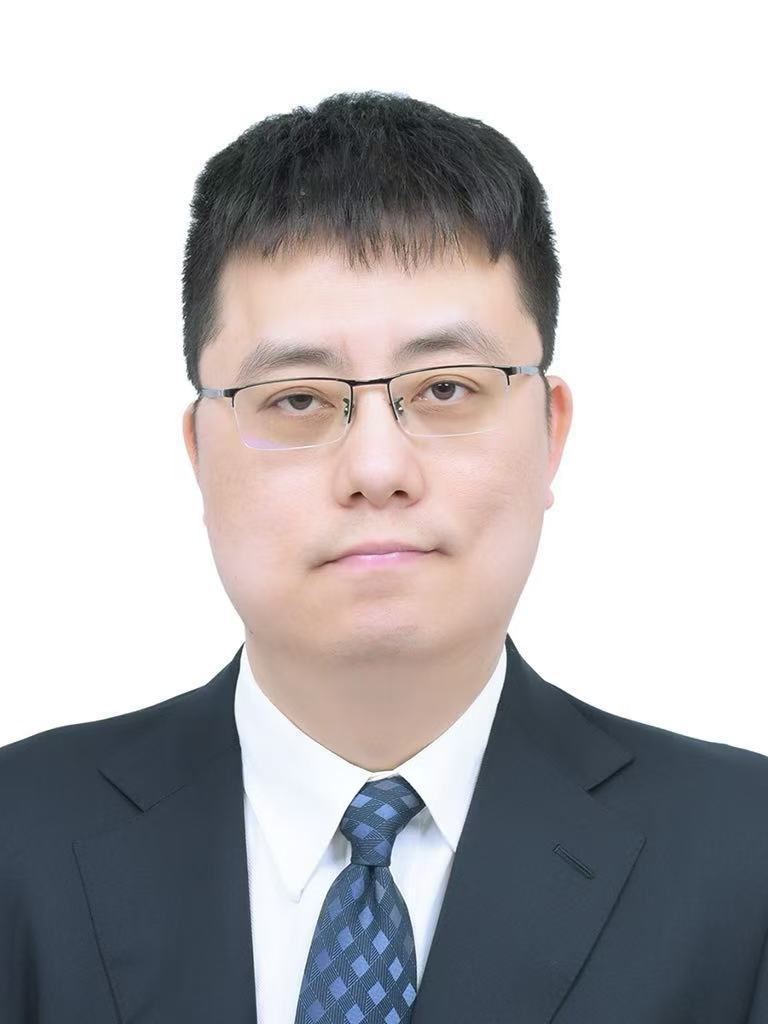
\includegraphics[width=1in,height=1.25in,clip,keepaspectratio]{fig/hh.jpg}}]{He Huang} (Senior Member, IEEE) received the Ph.D. degree from the School of Computer Science and Technology, University of Science and Technology of China (USTC), China, in 2011. He is currently a professor with the School of Computer Science and Technology, Soochow University, China. From 2019 to 2020, he was a visiting research scholar with Florida University, Gainesville. He has authored more than 100 papers in related international conference proceedings and journals. His current research interests include traffic measurement, computer networks, and algorithmic game theory. He is a member of the Association for Computing Machinery (ACM). He received the best paper awards from Bigcom 2016, IEEE MSN 2018, and Bigcom 2018. He has served as the Technical Program Committee member of several conferences, including IEEE INFOCOM, IEEE MASS, IEEE ICC, and IEEE Globecom.
\end{IEEEbiography}

\begin{IEEEbiography}[{
\includegraphics[width=1in,height=1.25in,clip,keepaspectratio]{fig/dhp.jpg}}]{Haipeng Dai} (Senior Member, IEEE) received the B.S. degree in the Department of Electronic Engineering from Shanghai Jiao Tong University, Shanghai, China, in 2010, and the Ph.D. degree in the Department of Computer Science and Technology in Nanjing University, Nanjing, China, in 2014. His research interests are mainly in the areas of edge computing, mobile computing, and data mining. He is a professor in School of Computer Science in Nanjing University. He has authored more than 300 papers in many prestigious conferences and journals such as USENIX NSDI, ACM UbiComp, IEEE INFOCOM, USENIX ATC, ACM EuroSys, ACM SIGMOD, ACM VLDB, IEEE ICDE, ACM SIGMETRICS, ACM MobiSys, ACM MobiHoc, IEEE ICNP, IEEE IPSN, IEEE TMC, IEEE JSAC, IEEE/ACM TON, IEEE TPDS, and IEEE TOSN. He is an IET Fellow, IEEE senior member, and ACM senior member. He serves/ed as the Leading Program Chair of IEEE ISPA'22-23, the Co-Vice Program Chair of IEEE HPCC'21, Track Chair of the ICCCN'19, ICPADS'21'25, and MSN'25. He served as TPC member of international conferences such as INFOCOM, IJCAI, SC, VLDB, SIGKDD, MobiHoc, and ICNP. He received Best Paper Award from IEEE ICNP'15, Best Paper Award Runner-up from IEEE SECON'18, Best Paper Award Candidate from IEEE INFOCOM'17, Best Paper Award from IEEE HPCC'22, Best Paper Award from WASA'22, and Distinguished Paper Award from ACM UbiComp'22.
\end{IEEEbiography}
\end{document}


